%!TEX options = --shell-escape
\documentclass[compress,10pt,dvipsnames]{Presentation}
% Add notesonly option to print the notes in each frame
% Add aspectratio=169 to do slides in 16 by 9 (some contents may need to be re-arranged)

\usepackage{MnSymbol,wasysym}
\usepackage{tcolorbox}
\tcbuselibrary{skins,raster}
\definecolor{mygray}{gray}{0.7}
\usepackage{svg}
\setsvg{inkscape=inkscape -z -D,svgpath=figures/}
\newcommand*{\ClipSep}{0.4cm}%

%%%%%%%%%%%%%%%%%%%%%%%%%%%%%%%%%%%%%%%%%%%%%%%%%%
%
% Some useful commands
%
\begin{comment}
Default Frame Size
12.8cm x 9.6cm (a 4:3 aspect ratio) with a font size of 11pt

    \frame
        {
            \frametitle{List displayed step-by-step}
            text
        }
      
    frame environment commands
    command<#>{applies the command only on certain slides}
    ex:
    \textbf{Thislineisboldonallthreeslides.}
    \textbf<2>{Thislineisboldsolelyonthesecondslide.}
    \textbf<3>{Thislineisboldsolelyonthethirdslide.}
      
    \only<#>{text shown only on the specified slide}
      
    \uncover<slides>{text that occupies space,but is not shown except on the specified slides}
      
    \invisible<slides>{text is invisible on the specified slides}
      
    \alt<slides>{<main text shown on specified slide>}{otherwise the alternative text is shown}
      
    \temporal<slides>{before specified slide}{on specified slide}{after specified slide}
      
    #-#
      
    #- all slides after #
      
    -#=1-#
      
    Highlighted environments
    \begin{beamerboxesrounded}{title}
    \end{beamerboxesrounded}
\end{comment}
%%%%%%%%%%%%%%%%%%%%%%%%%%%%%%%%%%%%%%%%%%%%%%%%%%

%\newsavebox\mybox
%\savebox\mybox{\tikz[color=red,opacity=0.3]\node{HOT OFF THE PRESS};}
%\newwatermark*[
%  pages=1,
%  angle=45,
%  scale=3,
%  xpos=-7,
%  ypos=8
%]{\usebox\mybox}

%%%%%%%%%%%%%%%%%%%%%%%%%%%%%%%%%%%%%%%%%%%%%%%%%%
\begin{comment}
%
% To show only one section and subsection at a time, uncomment this block
%
\setbeamertemplate{headline}
{%
  \leavevmode%
  \begin{beamercolorbox}[wd=.5\paperwidth,ht=2.5ex,dp=2.125ex]{section in head/foot}% original dp=1.125ex
    \hbox to .5\paperwidth{\hfil\insertsectionhead\hfil}
  \end{beamercolorbox}%
  \begin{beamercolorbox}[wd=.5\paperwidth,ht=2.5ex,dp=2.125ex]{subsection in head/foot}%
    \hbox to .5\paperwidth{\hfil\insertsubsectionhead\hfil}
  \end{beamercolorbox}%
}
\end{comment}
%%%%%%%%%%%%%%%%%%%%%%%%%%%%%%%%%%%%%%%%%%%%%%%%%%

\newcommand{\figpath}{/Users/aperloff/Documents/TAMU-Graduate/Thesis/DissertationDefense/figures/}
\newcommand{\anpath}{/Users/aperloff/Documents/CMS/Notes_and_Papers/notes/AN-13-132/trunk/figures/}
\newcommand{\qcdTalkPath}{/Users/aperloff/Documents/TAMU-Graduate/Research-RicardoEusebi/TAMUWW/Slides/2014_05_22-HWW-Alexx/}
\newcommand{\tikzmark}[1]{\tikz[overlay,remember picture] \node (#1) {};}

%%%%%%%%%%%%%%%%%%%%%%%%%%%%%%%%%%%%%%%%%%%%%%%%%%

\title[\HWWlvjj]{Search for a $125\unit{GeV}$ Standard Model Higgs boson decaying via \HWWlvjj} %\title[short title]{title}
\subtitle[Final Exam]{Dissertation Defense} %\subtitle[short subtitle]{subtitle}
\author[A. Perloff]{\textbf{Alexx Perloff\inst{1}}}
\institute[TAMU]
{
  \inst{1}%
  Department of Physics and Astronomy\\Mitchell Institute for Fundamental Physics \& Astronomy\\Texas A{\&}M University\\
  %College Station, Texas 77843\\[1ex]
  %\texttt{aperloff@physics.tamu.edu}
}
\newdate{date}{13}{12}{2017}
\date{\displaydate{date}}
%\date{\today}

%%%%%%%%%%%%%%%%%%%%%%%%%%%%%%%%%%%%%%%%%%%%%%%%%%
\begin{document}

%\beamertemplatenavigationsymbolsempty
\newlength{\residualSpace}

\frame {
    \vspace{-0.4cm}
    \begin{center}
        \makebox[0pt][l]{
\includegraphics[width=0.50in]{figures/TAMULogoMaroonBox.jpg}}\hfill%
        \makebox[0pt][r]{
\includegraphics[width=0.50in]{figures/CMS_exp.png}}
    \end{center}
    \vspace{-0.8cm}
    \titlepage
}

{
\usebackgroundtemplate{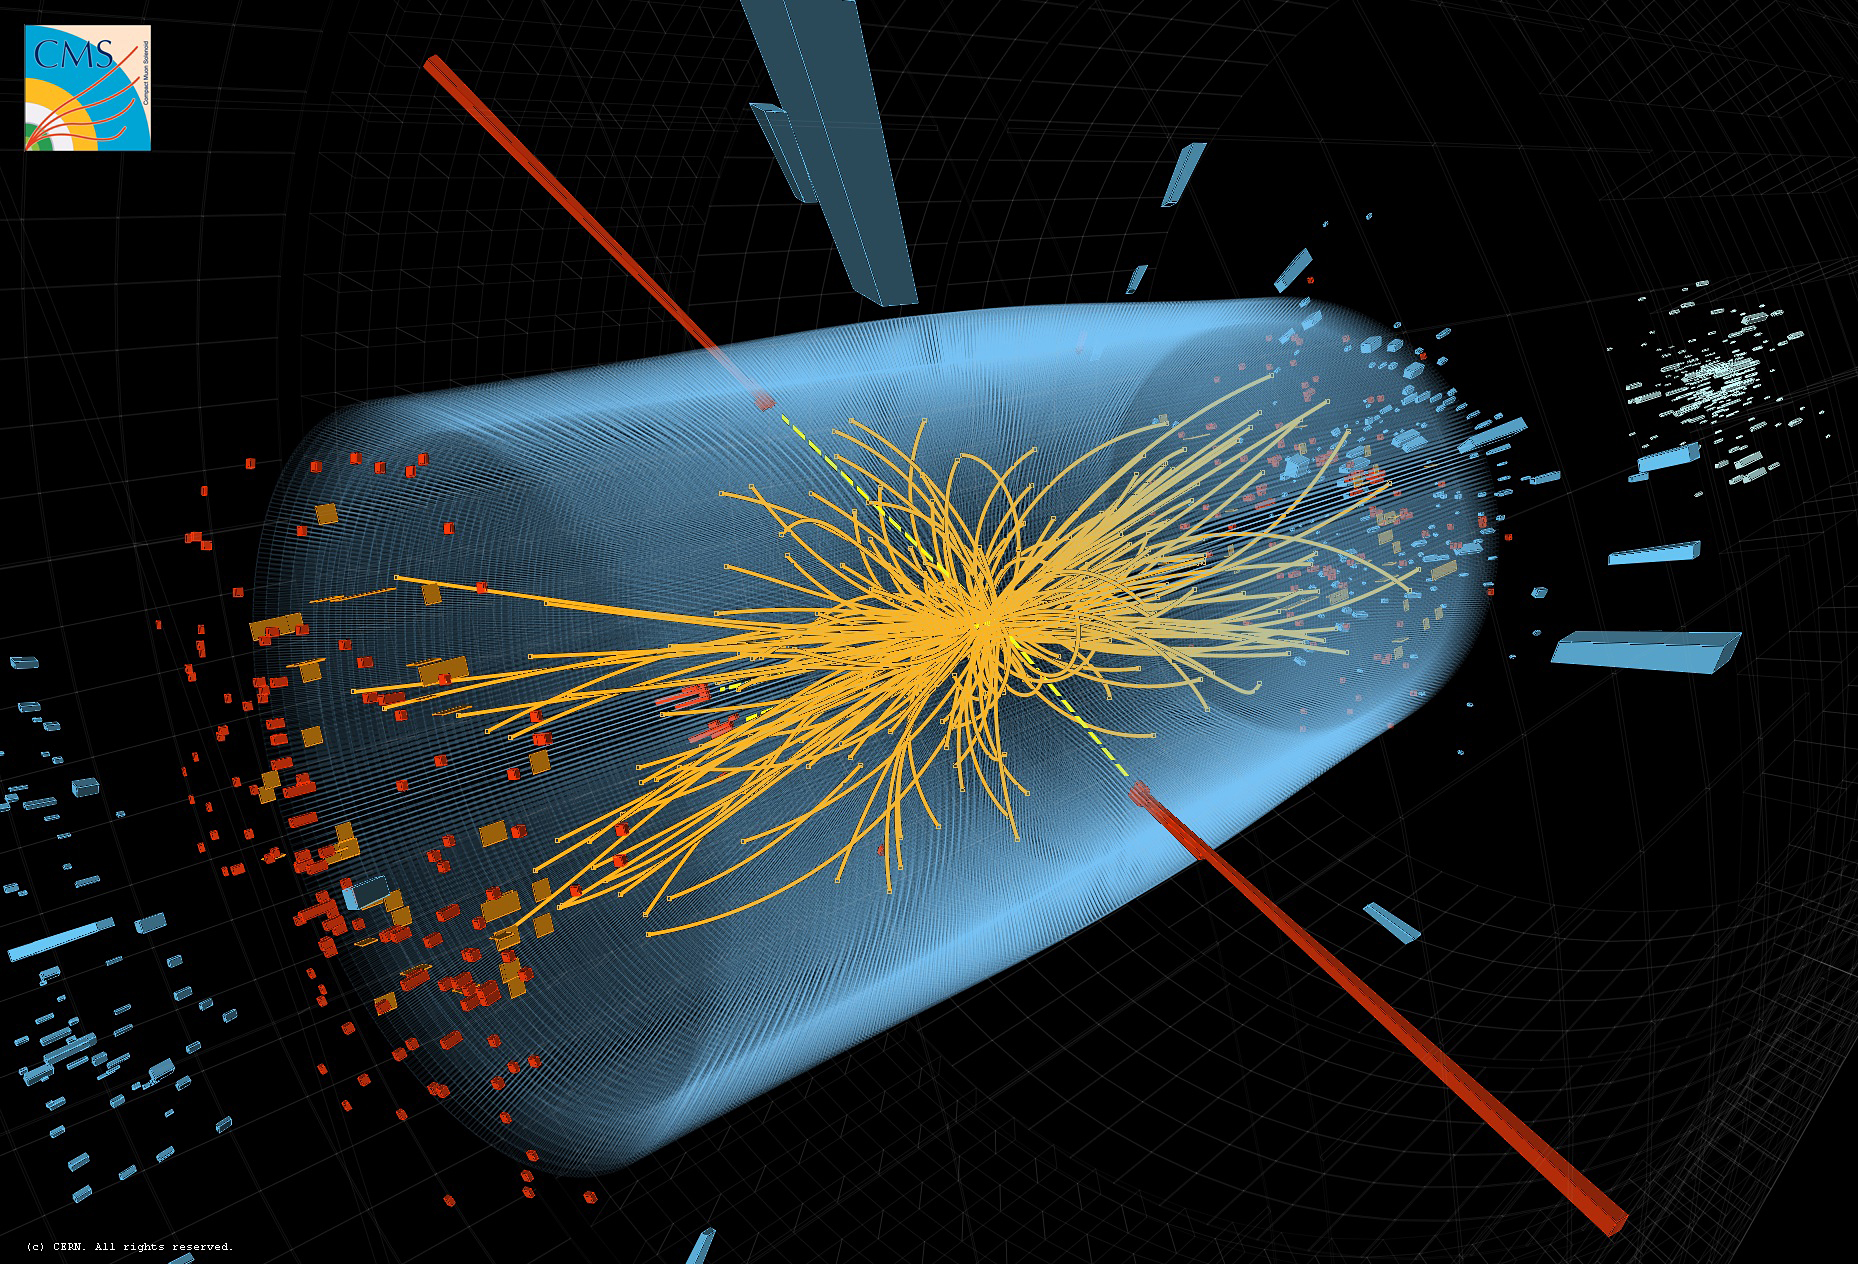
\includegraphics[width=\paperwidth,height=\paperheight]{\figpath/cms-image1112.jpg}}%
\setbeamercolor{section in toc shaded}{use=structure,fg=structure.fg}
\setbeamercolor{section in toc}{fg=white}
\setbeamercolor{subsection in toc shaded}{fg=black}
\setbeamercolor{subsection in toc}{fg=white}
%\frame<beamer>{\begin{multicols}{2}
%    \frametitle{Outline}
%    \setcounter{tocdepth}{2}  
%    \tableofcontents
%\end{multicols}}
%
\begin{frame}
    \setbeamerfont{subsection in toc}{size=\large,series=\bf}
    \setbeamerfont{section in toc}{size=\Large,series=\bf}
    \frametitle{Outline}
    \vspace*{-0.42cm}
    \hspace*{-2cm}%
    
\begin{tikzpicture}
      \draw[draw=black,fill=black] (0,0) rectangle (15,0.15);
    \end{tikzpicture}

    \tableofcontents[sections={1-8}]
%    \begin{columns}[t]
%        \begin{column}{.5\textwidth}
%            \tableofcontents[sections={1-3}]
%        \end{column}%
%        \begin{column}{.5\textwidth}
%            \vspace*{-1.5cm}
%            \tableofcontents[sections={4-7}]
%        \end{column}
%    \end{columns}
\end{frame}
}

\section[Intro.]{Introduction}
\label{sec:intro}
%!TEX root = ../DissertationDefensePresentation.tex

%%--------------------------------------------------------------------------------------------

\subsection{Standard Model}

%%--------------------------------------------------------------------------------------------

\begin{frame}[fragile]
	\tikzstyle{myarrows}=[line width=1mm,draw=magenta,-triangle 45,postaction={draw, line width=3mm, shorten >=4mm, -}]
	\frametitle{The Standard Model: Particle Physics In A Nutshell}
	\vspace*{-0.24cm}
	\begin{block}{}
		\begin{columns}[t,onlytextwidth]
			\column{0.52\textwidth}
			\vspace*{-0.20cm}
			\begin{itemize}
				\small
				\item $SU(3)_{C}{\otimes}SU(2)_{L}{\otimes}U(1)_{Y}$ gauge theory
				\item Forces are mediated by spin-1 gauge bosons (4).
				\begin{itemize}
					\item $\gamma$\enspace- electromagnetic interactions
					\item \Wpm/\cPZ\enspace- weak interactions
					\item \cPg\enspace- strong interactions
				\end{itemize}
			\end{itemize}
			\column{0.51\textwidth}
			\begin{itemize}
				\vspace*{-0.20cm}
				\small
				\item Matter is made up of spin-1/2 fermions
				\begin{itemize}
					\item Leptons (6) and quarks (6)
				\end{itemize}
				\item Spin-0 \textbf{Higgs boson}
				\begin{itemize}
					\item Responsible for the mass of the fundamental particles
				\end{itemize}
			\end{itemize}
		\end{columns}
	\end{block}
	\vspace*{-0.6cm}
	\begin{columns}[T]
		\begin{column}{0.75\textwidth}
	\begin{figure}
		\resizebox{0.82\textwidth}{!}{\input{StandardModel_CERNWebfest2012}}
		\label{fig:standard_model}
	\end{figure}
		\end{column}
		\begin{column}{0.25\textwidth}
			\vspace*{3.75cm}
			Explains \textbf{many} of the properties of the known universe, but not all of them
		\end{column}
	\end{columns}
	\begin{textblock}{0.01}(0.575,0.555)
		\tikz[baseline,remember picture]{\node[coordinate] (t1) {};}
	\end{textblock}
	\begin{textblock}{0.2}(0.75,0.53)
		\tikz[remember picture]{\node[coordinate] (n1) {};}Observation announced July 4th, 2012
		\begin{tikzpicture}[remember picture,overlay]   %% use here too
        	%\path[draw=magenta,thick,->] (n1.west) to (t1.east);
        	\path[myarrows] ([xshift=-2mm]n1.west) to (t1.east);
		\end{tikzpicture}
	\end{textblock}
\end{frame}

\begin{frame}
	\frametitle{Physics Beyond the Standard Model (BSM)}
	\vspace*{-0.24cm}
	%\begin{block}{Why mention BSM?}
	\begin{block}{What is the SM lacking?}
		\begin{itemize}
			\item A dark matter candidate
			\item A way to explain non-zero neutrino mass and neutrino oscillations
			\item A theory of gravity
			\item An explanation for the matter-antimatter asymmetry of the universe
		\end{itemize}
	\end{block}
	\vspace*{-0.15cm}
	\begin{figure}
		\label{fig:BSM}
		\centering
		\begin{subfigure}[t]{0.20\textwidth}
			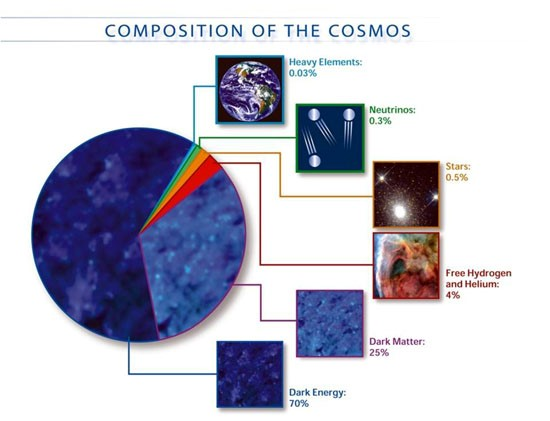
\includegraphics[width=\textwidth]{\figpath/CosmicComposition.jpg}
			\label{fig:BSM1}
		\end{subfigure}
		\hfill
		\begin{subfigure}[t]{0.21\textwidth}
			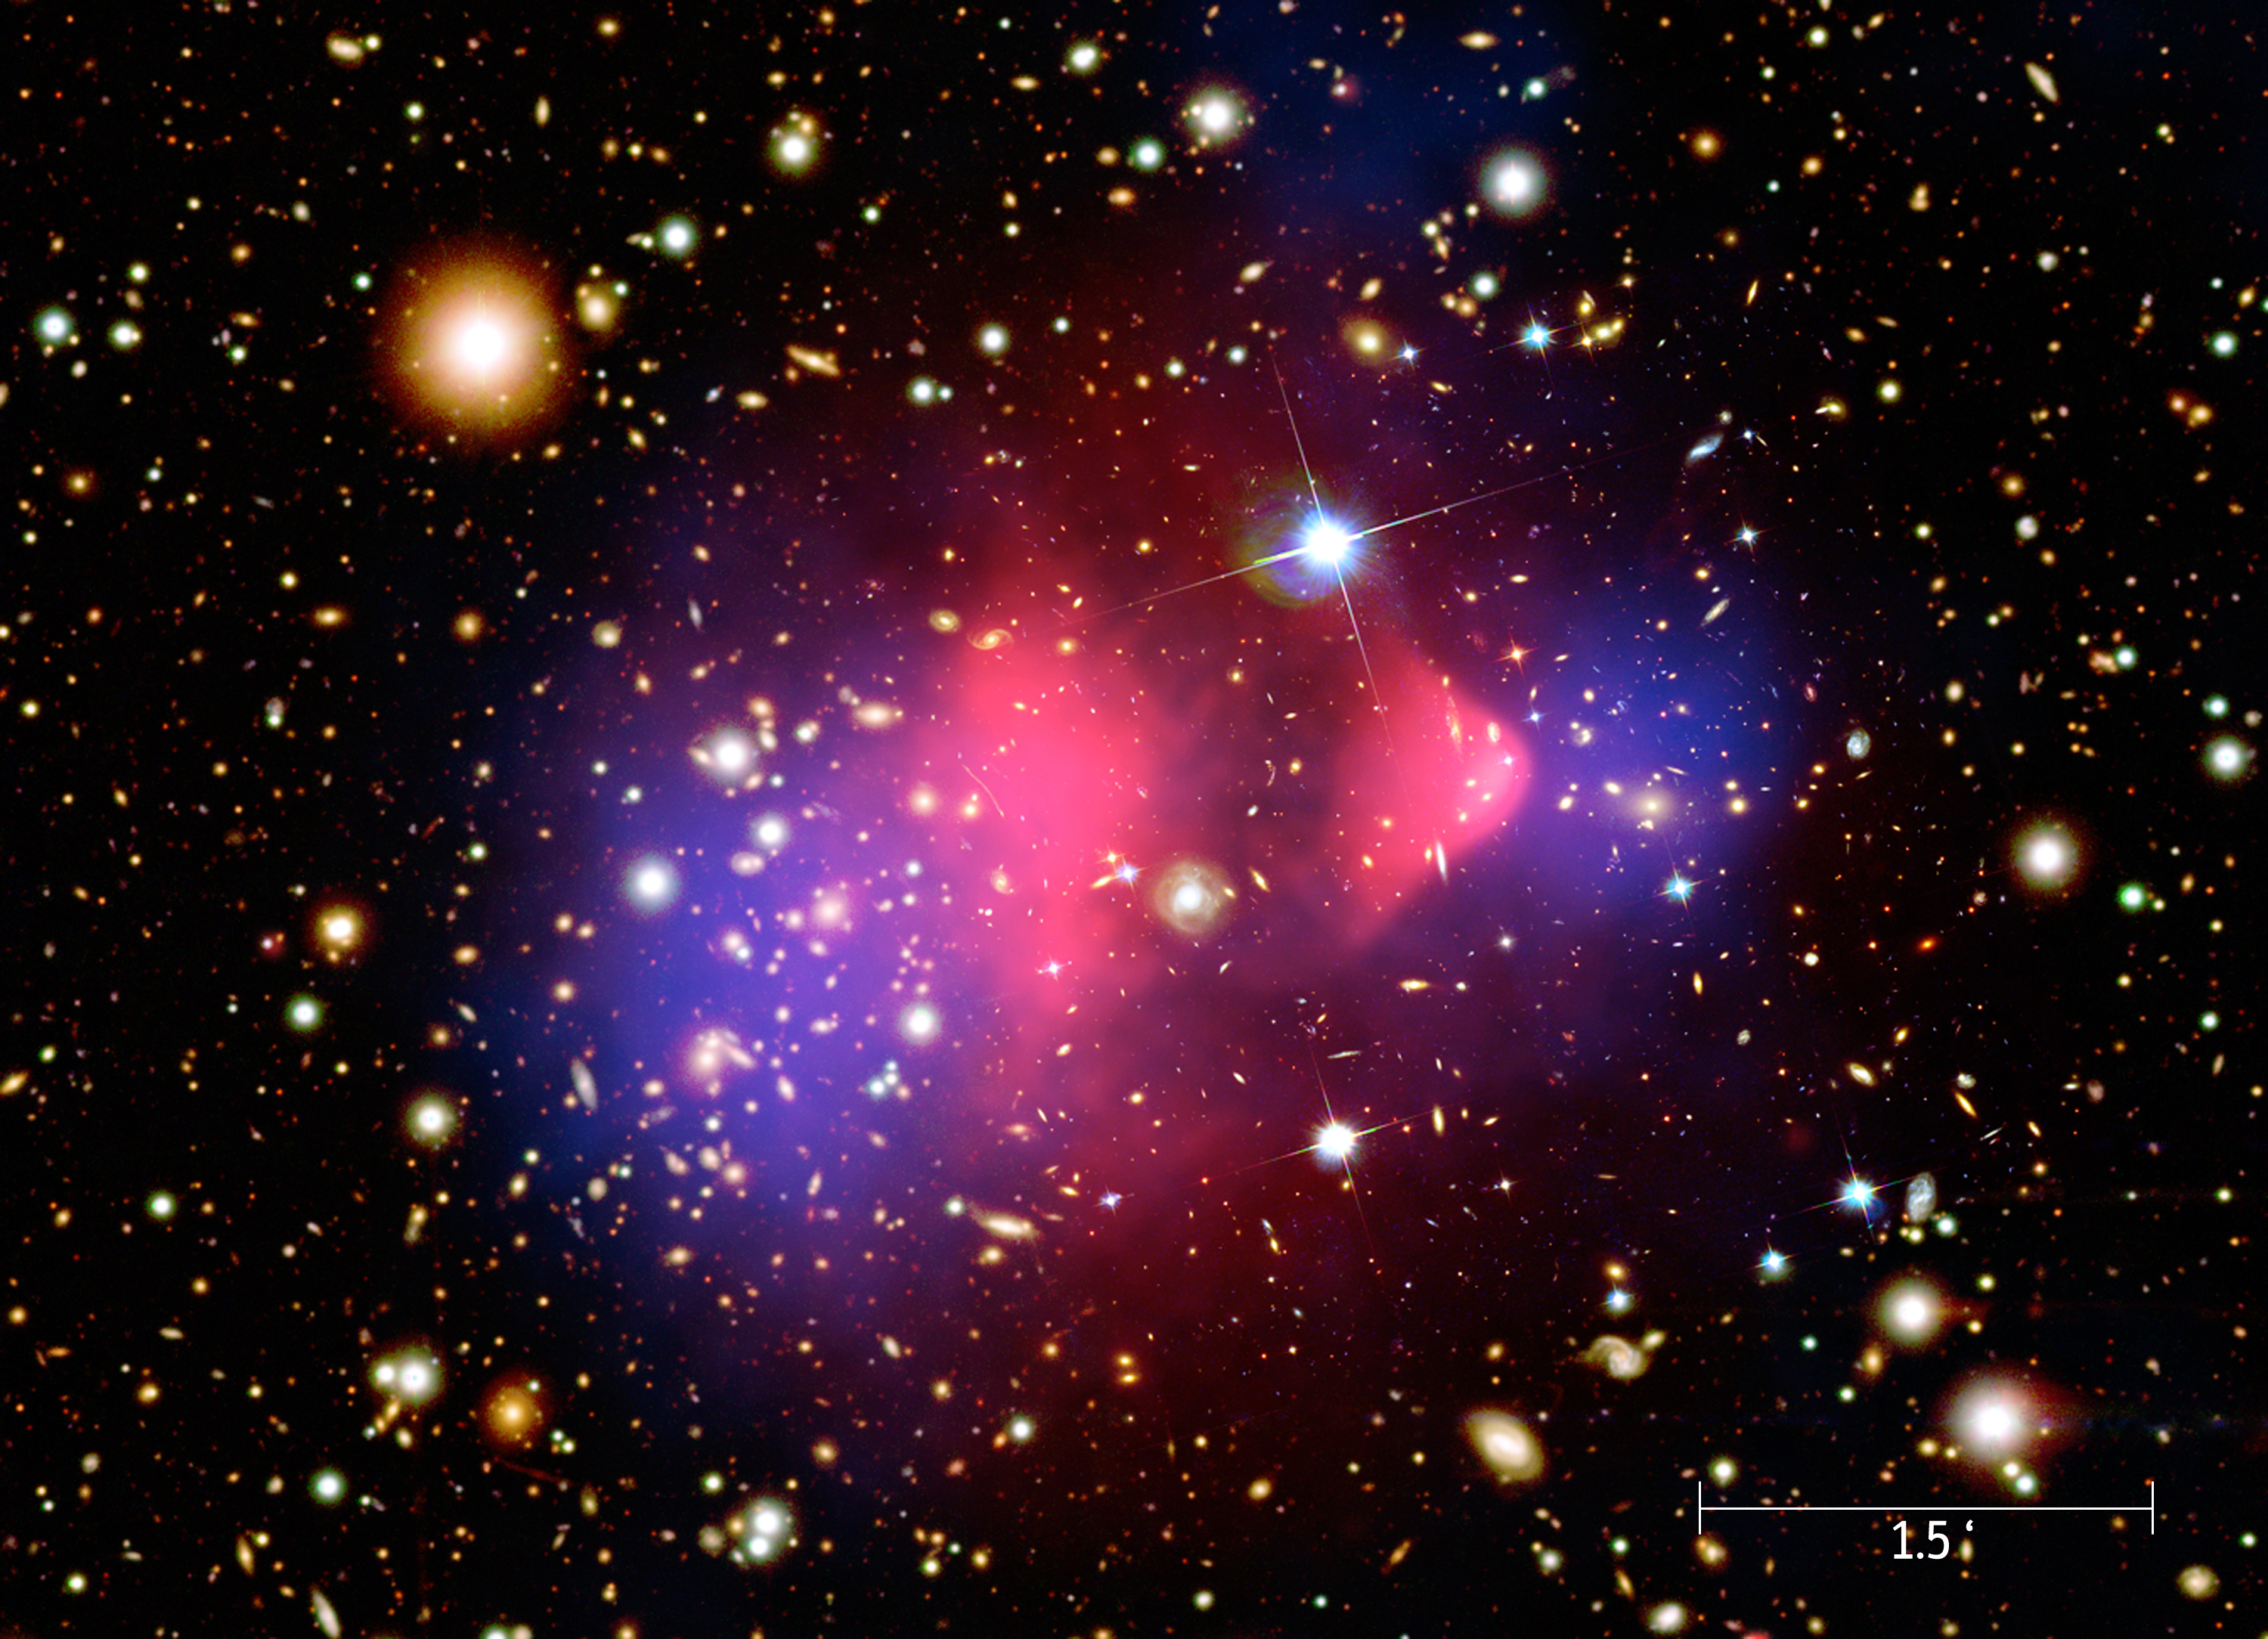
\includegraphics[width=\textwidth]{\figpath/bullet_clusters.jpg}
			\label{fig:BSM2}
		\end{subfigure}
		\hfill
		\begin{subfigure}[t]{0.20\textwidth}
			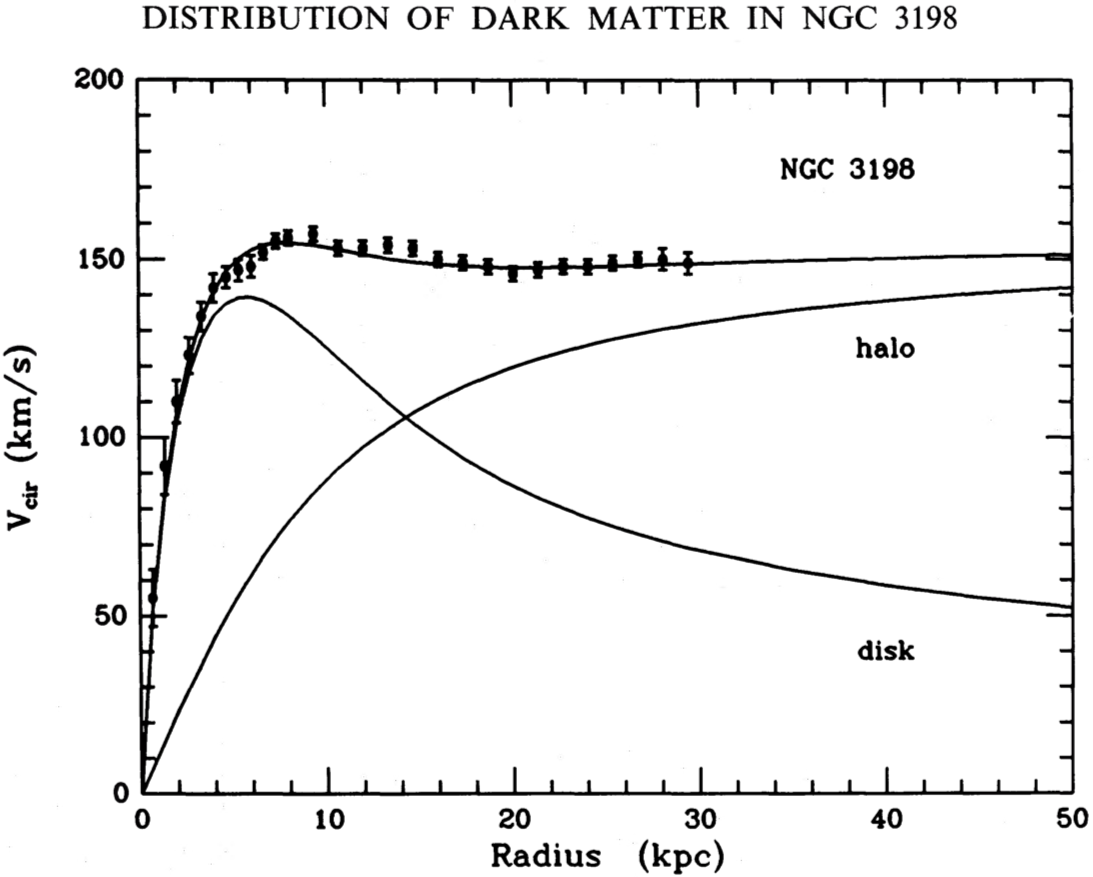
\includegraphics[width=\textwidth]{\figpath/GalaxyHalo.png}
			\label{fig:BSM3}
		\end{subfigure}
		\hfill
		\begin{subfigure}[t]{0.24\textwidth}
			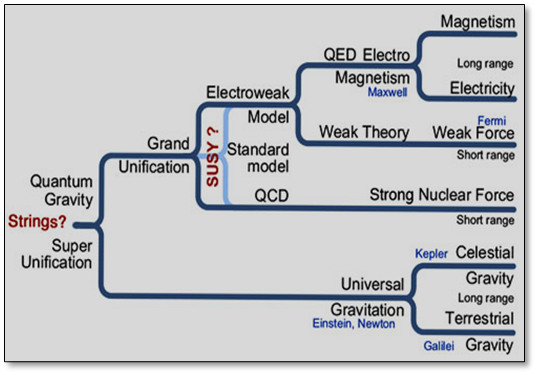
\includegraphics[width=\textwidth]{\figpath/unification.png}
			\label{fig:BSM4}
		\end{subfigure}
	\end{figure}
	\vspace*{-0.30cm}
	\begin{block}{What does Higgs physics have to do with BSM?}
		\begin{itemize}
			\item Need at least one (SM Higgs) to provide mass to particles
			\begin{itemize}
				\item Study the properties of SM Higgs boson, especially its couplings
			\end{itemize}
			\item Additional particles in the Higgs sector at the $\mathcal{O}\left(1 TeV\right)$ scale would be proof of BSM physics
			\begin{itemize}
				\item Could disambiguate supersymmetry (SUSY), from composite Higgs models, etc.
			\end{itemize}
			%\item If we have really observed ``the'' standard model Higgs boson, then we should be able to find it in all decay channels
			%\item If it's not there ($l{\nu}jj$), then either the model is again defficient or we didn't observe the boson we thought we had
			%\item So we must either search for or set limits on the Higgs SM branching ratios
		\end{itemize}
	\end{block}
\end{frame}

\begin{frame}
	\tikzstyle{na} = [baseline=-.5ex]
	\frametitle{Higgs Production}
	\vspace*{-0.8cm}
	\begin{center}
		\begin{tikzpicture}[remember picture]%,show background grid]
            % Put the graphic inside a node. This makes it easy to place the
            % graphic and to draw on top of it. 
            % The above right option is used to place the lower left corner
            % of the image at the (0,0) coordinate. 
            \node [inner sep=0pt,above right] 
                {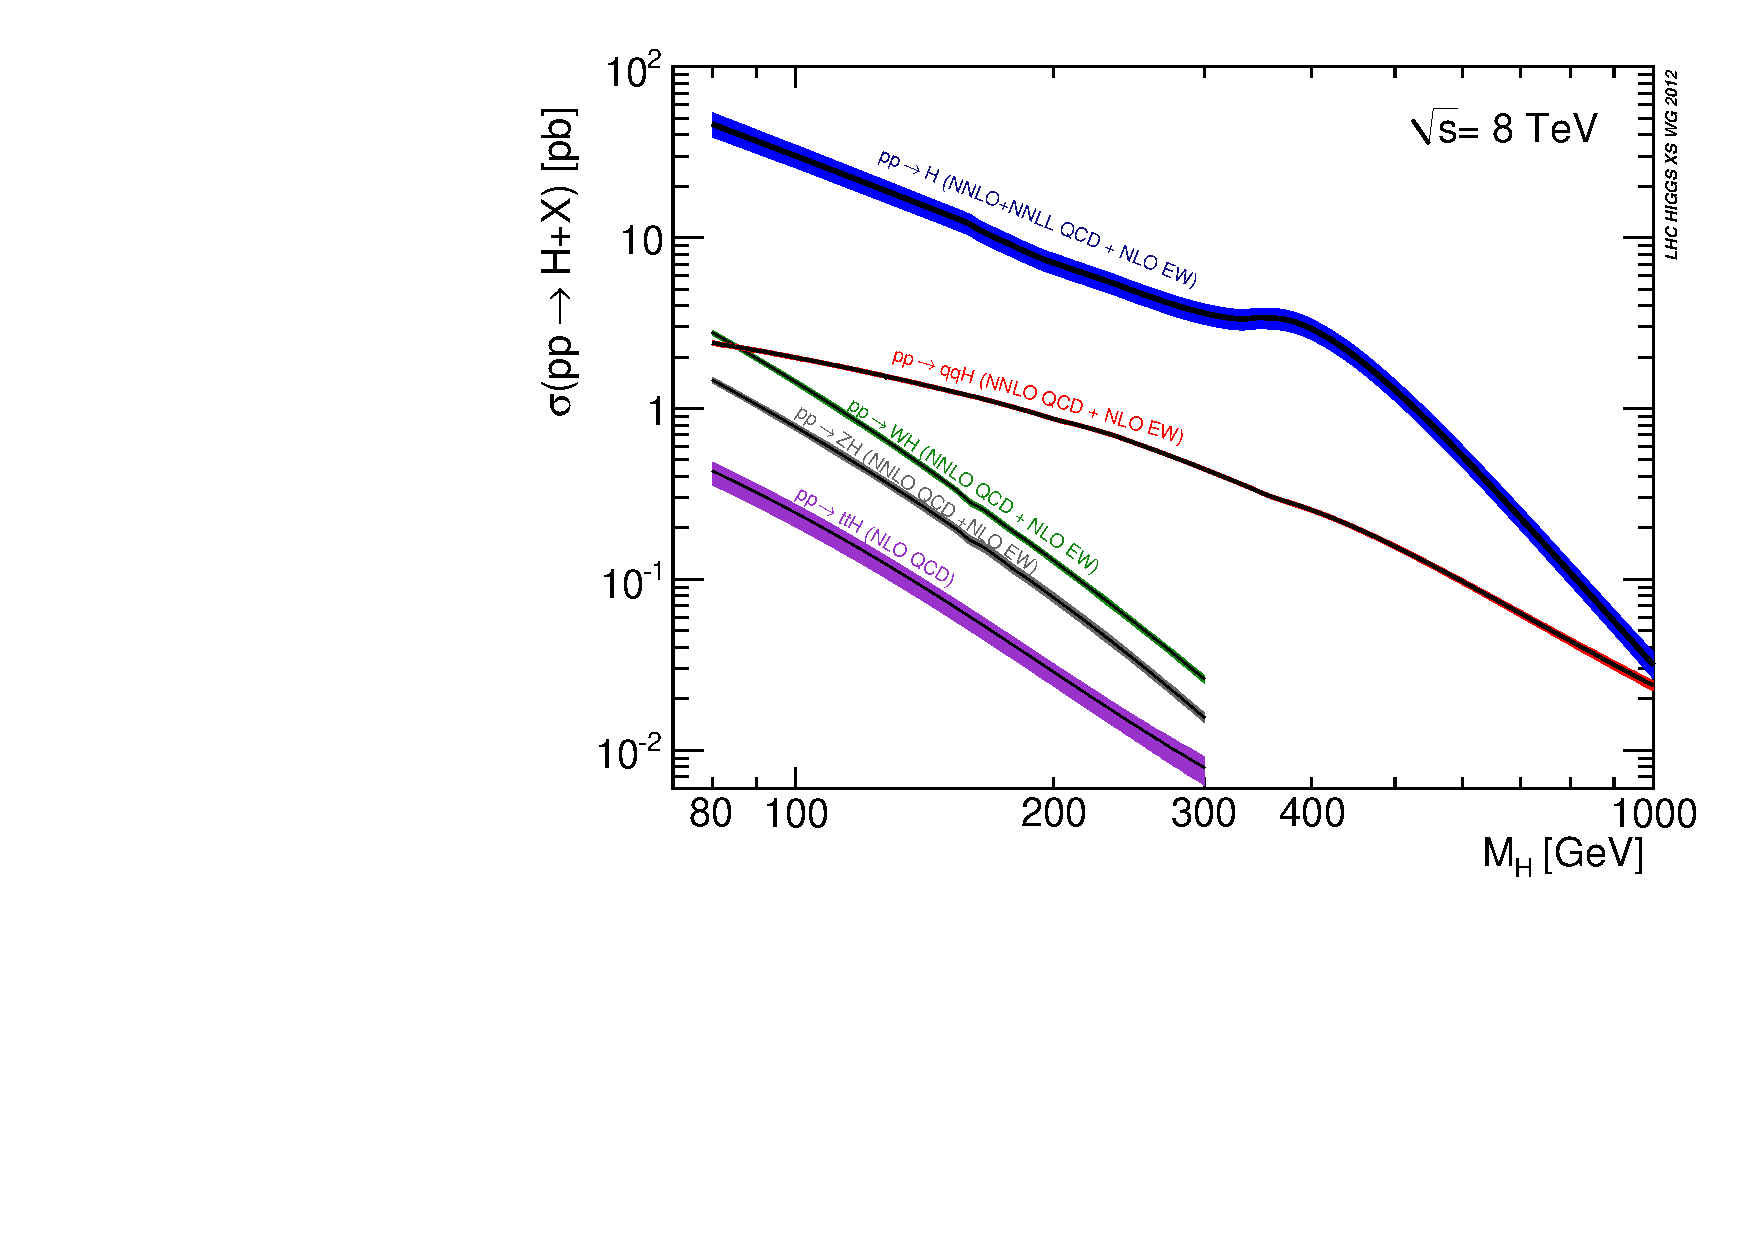
\includegraphics[width=0.65\textwidth]{\figpath/Higgs_XS_8TeV_lx.pdf}};
            % show origin
            \fill (0,0) circle (2pt);
            % define destination coordinates
            \path (6.3,3.2) coordinate (ggH)
                  (6.2,2.0) coordinate (qqH)
                  (1.5,3.5) coordinate (WH)
                  (3.0,1.6) coordinate (ttH);
        \end{tikzpicture}
	\end{center}
	\vfill

	\begin{textblock}{0.24}(0.74,0.32)
		\begin{tcolorbox}[colframe=blue,colback=blue!20!white]
			\tikz[remember picture, na] \coordinate (s-ggH);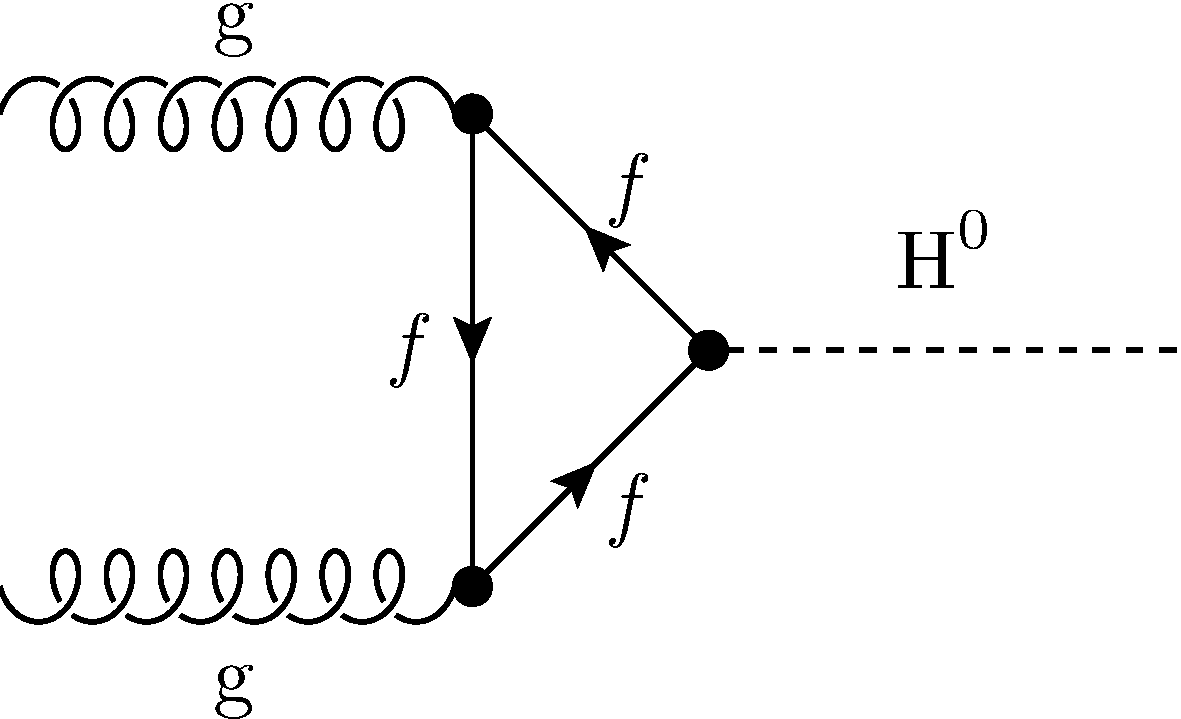
\includegraphics[width=\textwidth]{\figpath/FeynmanDiagrams/ggH.pdf}
			%\tiny \HWW
		\end{tcolorbox}
	\end{textblock}
	\begin{textblock}{0.24}(0.55,0.75)
		\begin{tcolorbox}[colframe=red,colback=red!20!white]
			\tikz[remember picture, na] \coordinate (s-qqH);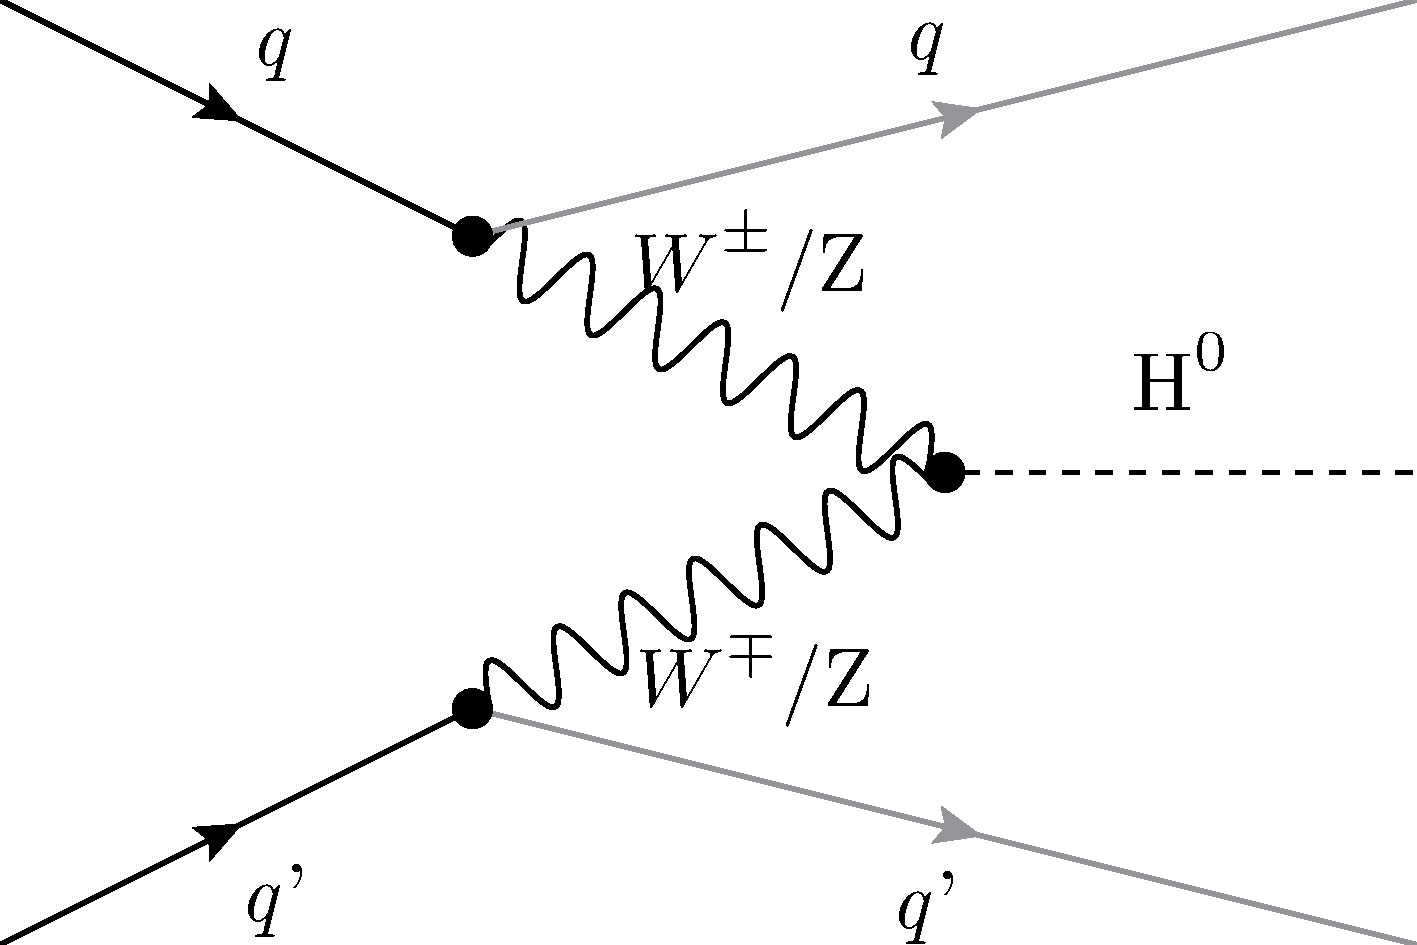
\includegraphics[width=\textwidth]{\figpath/FeynmanDiagrams/qqH.pdf}
			%\tiny \HWW
		\end{tcolorbox}
	\end{textblock}
	\begin{textblock}{0.24}(0.005,0.46)
		\begin{tcolorbox}[colframe=green,colback=green!20!white]
			\tikz[remember picture, na] \coordinate (s-WH);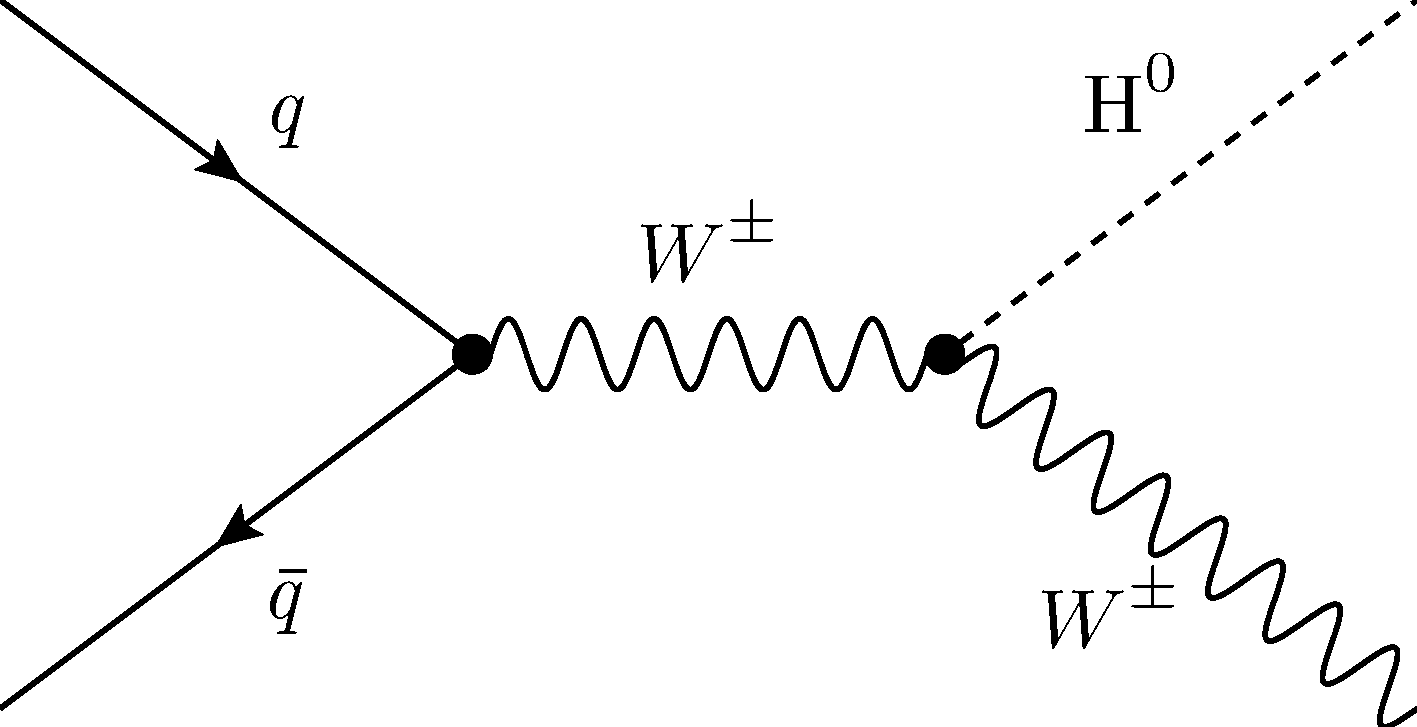
\includegraphics[width=\textwidth]{\figpath/FeynmanDiagrams/WH.pdf}
			%\tiny \HWW, \HZZ, \Hbb (\Wlv)
		\end{tcolorbox}
	\end{textblock}
	\begin{textblock}{0.24}(0.005,0.73)
		\begin{tcolorbox}[colframe=violet,colback=violet!20!white]
			\tikz[remember picture, na] \coordinate (s-ttH);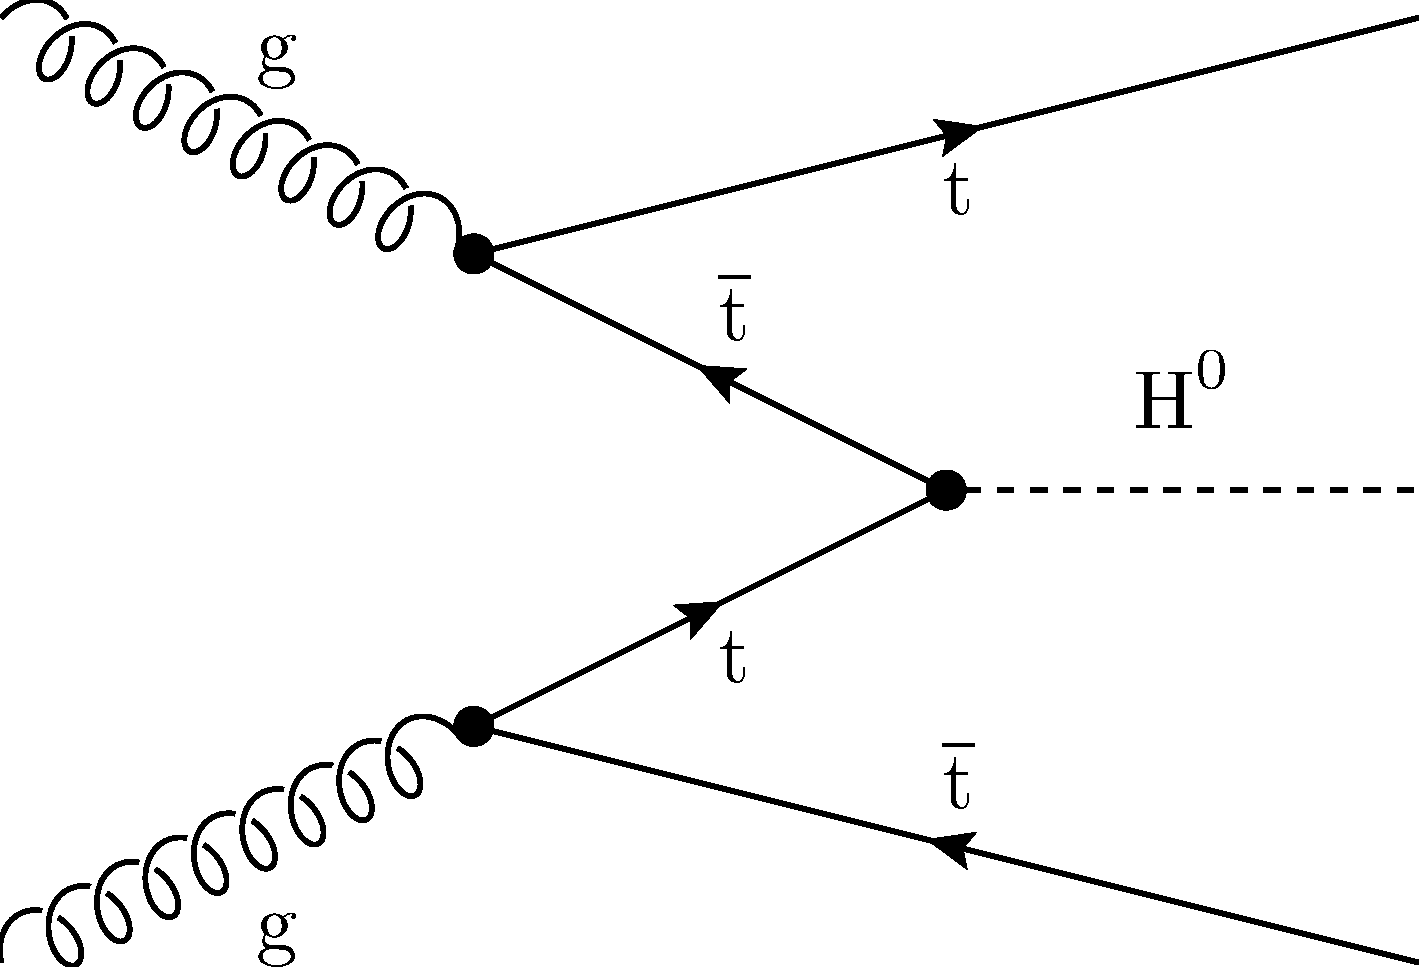
\includegraphics[width=\textwidth]{\figpath/FeynmanDiagrams/ttH.pdf}
			%\tiny \HWW, \HZZ, \Hbb
		\end{tcolorbox}
	\end{textblock}

	\begin{textblock}{0.24}(0.745,0.49)
		\tiny Gluon-Gluon Fusion
	\end{textblock}
	\begin{textblock}{0.24}(0.555,0.93)
		\tiny Vector-Boson Fusion
	\end{textblock}
	\begin{textblock}{0.24}(0.01,0.61)
		\tiny Associated Production
	\end{textblock}
	\begin{textblock}{0.24}(0.01,0.91)
		\tiny \ttbar Fusion
	\end{textblock}
	
	% define overlays
	% Note the use of the overlay option. This is required when 
	% you want to access nodes in different pictures.
	\begin{tikzpicture}[remember picture,overlay]
	        \path[->,blue,thick] ([yshift=5mm]s-ggH) edge (ggH);
	        \path[->,red,thick] ([xshift=1.9cm]s-qqH) edge [bend left] (qqH);
	        \path[->,green,thick] ([yshift=5mm]s-WH) edge [bend right] (WH);
	        \path[->,violet,thick] (s-ttH) edge [out=0, in=-90] (ttH);
	\end{tikzpicture}
\end{frame}

%%--------------------------------------------------------------------------------------------

\subsection[Motivation]{Motivation}

%%--------------------------------------------------------------------------------------------

\begin{frame}
	\frametitle{Higgs Decay}
	\framesubtitle{\small Why search for the Higgs boson in the \HWWlvjj channel?}
	\vspace*{-0.24cm}	
	\begin{columns}[T]
		\column{0.64\textwidth}
			\vspace*{-0.25cm}
			\begin{block}{}
				\begin{itemize}
					\item \HWW analyses:
					\begin{itemize}
						\item Probe the \HWW vertex directly
						\item One of the highest branching ratios
					\end{itemize}
					\item Fully-leptonic analysis (\HWWlvlv)
					\begin{itemize}
						\item Only channel to probe vertex, so far ($\sim$4$\sigma$ result)
						\item Would be nice to have another handle to probe this vertex
					\end{itemize}
					\item \textbf{Semi-leptonic analysis} (\HWWlvjj)
					\begin{itemize}
						\item The good:
						\begin{itemize}
							\item High $\sigma\times$BR for $\MH\sim$125\GeV
							\item Has a reconstructible Higgs boson mass peak
						\end{itemize}
						\item The bad:
						\begin{itemize}
							\item Looked at only for $\MH>\text{2}\MW$
							%\item Searching in the WW channel requires one W to be off-shell since $M_{H}<2M_{W}$
							\item Small signal to background ratio
							%\item The resolution in the semileptonic channel is not as good as the fully-leptonic channel due to the presence of jets and MET
						\end{itemize}
						\item New techniques may make this channel feasible and useful for measuring the properties of the Higgs boson
					\end{itemize}
				\end{itemize}
			\end{block}
		\column{0.015\textwidth}
		\column{0.33\textwidth}
			\vspace*{-0.33cm}
			\begin{myfancyblock}
				\node[anchor=south west,inner sep=0] (image) at (0,0) {%
					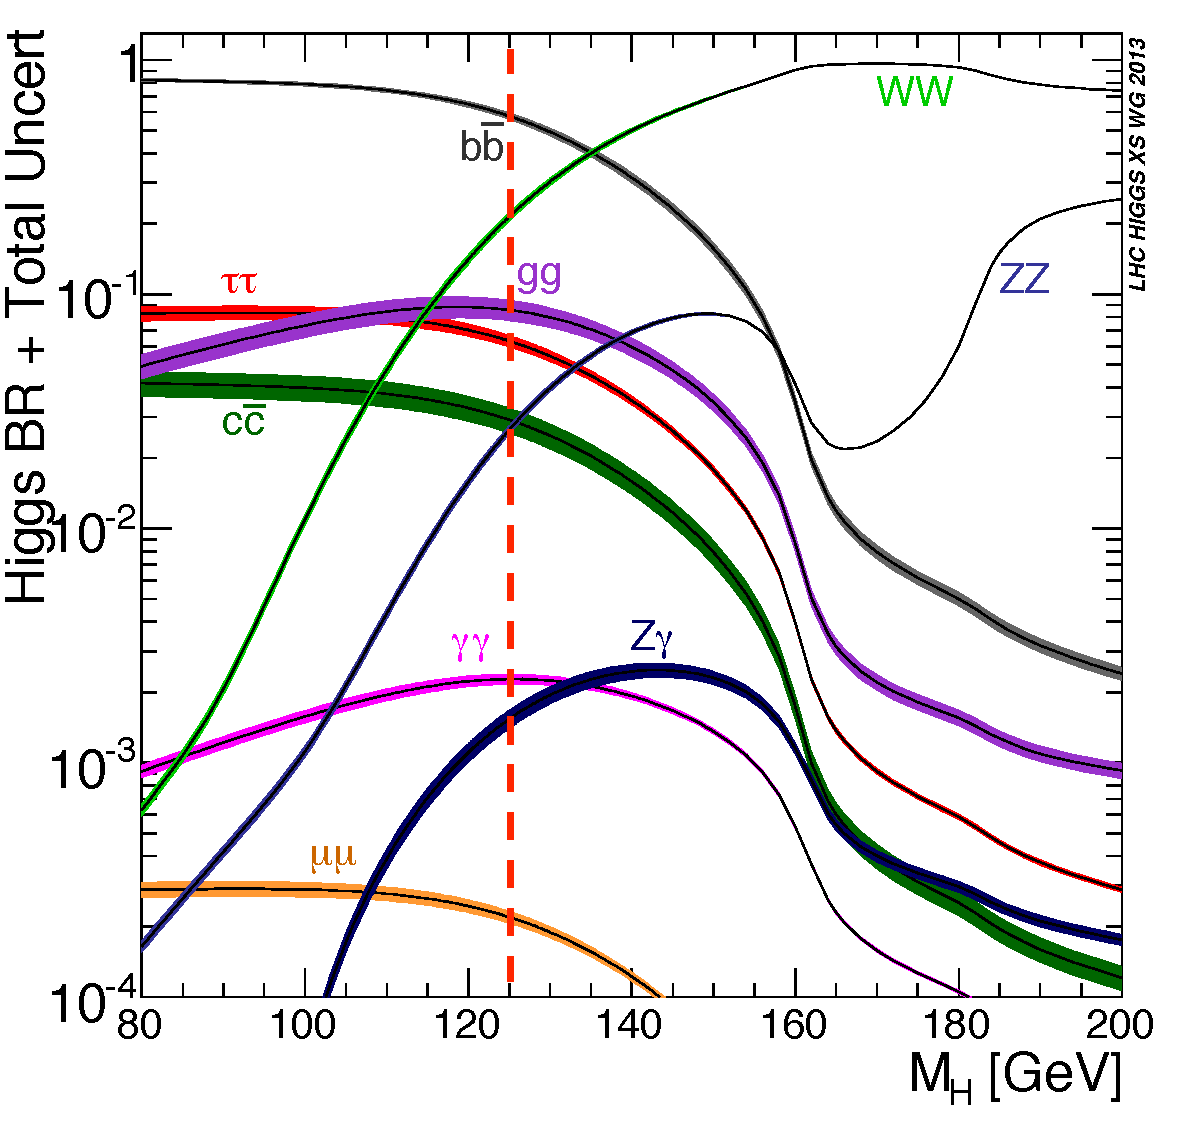
\includegraphics[width=\textwidth]{\figpath/Higgs_BR_LM.pdf}
				};
				\node[anchor=south west,inner sep=0] (image2) at (0,-3.9) {%
					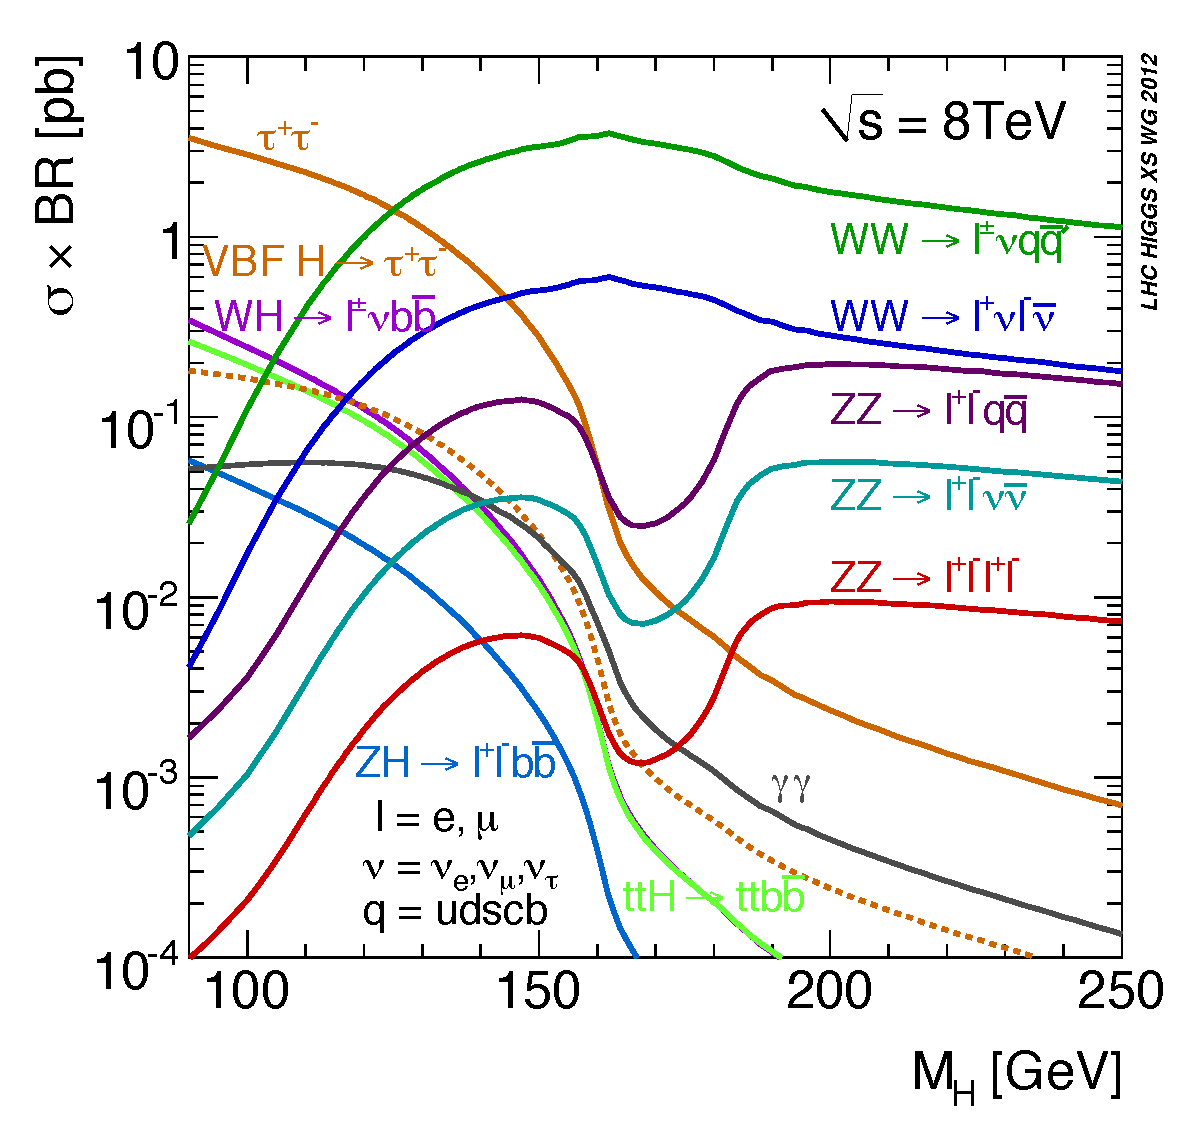
\includegraphics[width=\textwidth]{\figpath/XSBR_8TeV_SM_LM}
				};
				\draw[orange,thick] (1.755,3.78) -- (1.755,0.465);
				\draw[orange,thick] (1.38,-0.17) -- (1.38,-3.27);
			\end{myfancyblock}

			%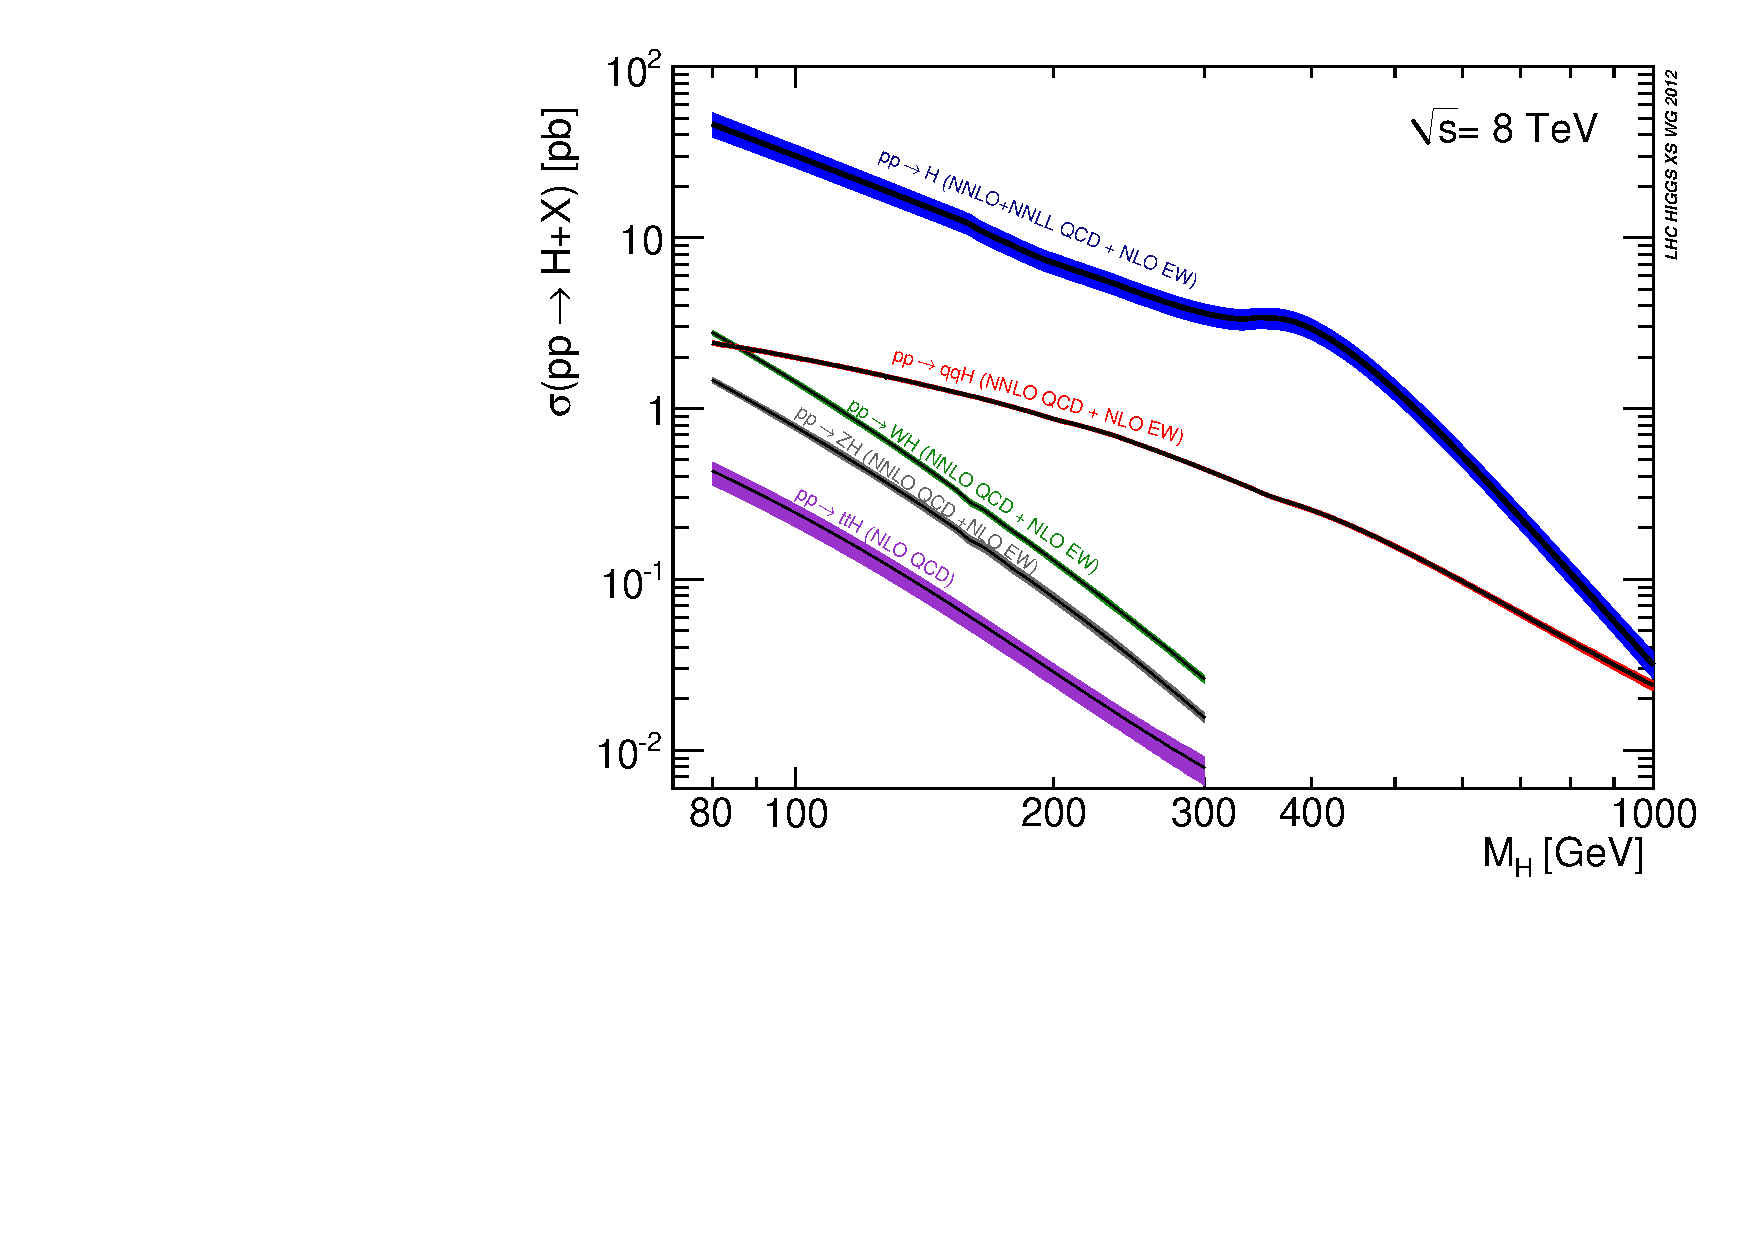
\includegraphics[width=\textwidth]{\figpath/Higgs_XS_8TeV_lx.pdf}\\
			%\vspace*{-0.1cm}
			%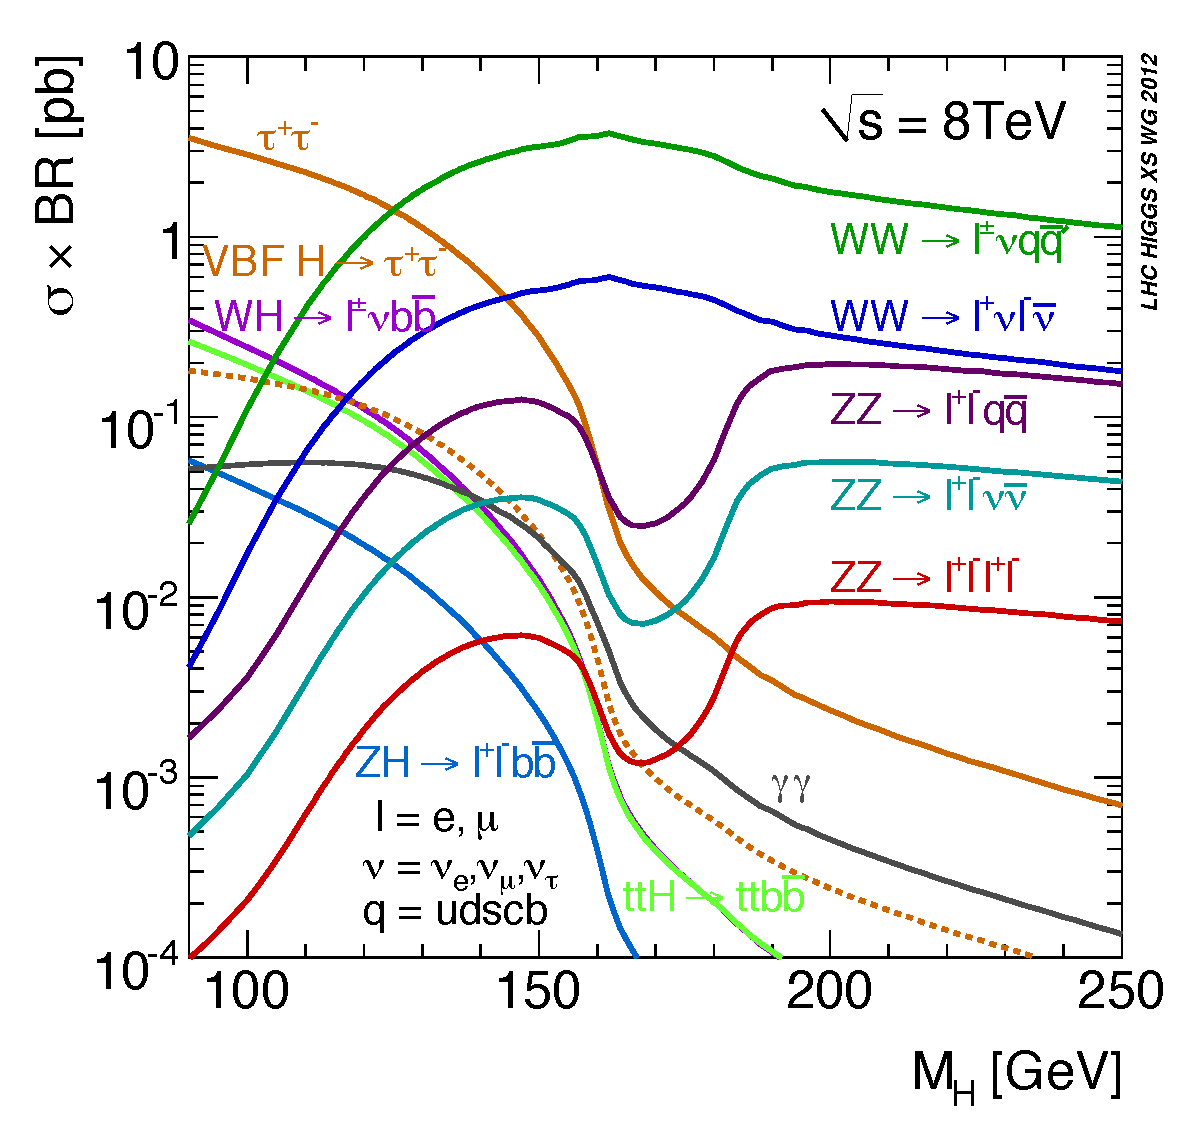
\includegraphics[width=\textwidth]{\figpath/XSBR_8TeV_SM_LM}
	\end{columns}
\end{frame}


\addtocontents{toc}{\vskip 0.5cm}
\section[Facilities]{Experimental Facilities}
\label{sec:experiment}
%!TEX root = ../DissertationDefensePresentation.tex

{
\usebackgroundtemplate{
  
\begin{tikzpicture}
    \path [outer color = white, inner color = gray!85]
      (0,0) rectangle (\paperwidth,\paperheight);
  \end{tikzpicture}}
\begin{frame}
    \begin{textblock}{1.0}(0.00,0.20)
        \begin{tcbraster}[raster columns=2,raster force size=false,size=fbox]
            \begin{center}
                \tcbincludegraphics[blank,arc=\ClipSep,hbox,graphics options={width=0.4\textwidth}]{\figpath/1280px-CERN-aerial_1.jpg}\hspace*{0.1cm}\tcbincludegraphics[blank,arc=\ClipSep,hbox,graphics options={width=0.4\textwidth}]{\figpath/CMS_detector-s.jpg}
            \end{center} 
        \end{tcbraster}
    \end{textblock}
    \begin{textblock}{1.0}(0.0,0.75)
        \begin{center}
            \Huge
            Experimental Facilities\\
            \large
            CERN, the LHC, and CMS
        \end{center}
    \end{textblock}
\end{frame}
}

%%--------------------------------------------------------------------------------------------

\subsection*{CERN}

%%--------------------------------------------------------------------------------------------

\begin{frame}
    \frametitle{CERN}
    \framesubtitle{European Organization for Nuclear Research}
    \vspace*{-0.44cm}
    \begin{columns}[T]
        \begin{column}{0.4\textwidth}
            \begin{block}{}
                \begin{itemize}
                    \item One of the world's premier particle physics laboratories
                    \begin{itemize}
                        \item Founded in 1954
                        \item Currently supported by 22 member states
                        \item Located along the French-Swiss border near Geneva, Switzerland
                        \item Many discoveries: \PW, \PZ, and \PH bosons, World Wide Web, etc.
                    \end{itemize}
                    \vspace*{0.2cm}
                    \item A huge underground accelerator complex supports the largest of the beamlines, the Large Hadron Collider (LHC)
                \end{itemize}
            \end{block}
        \end{column}
        \begin{column}{0.58\textwidth}
            \centering
            \vspace*{1.0cm}
            \hspace*{0.1cm}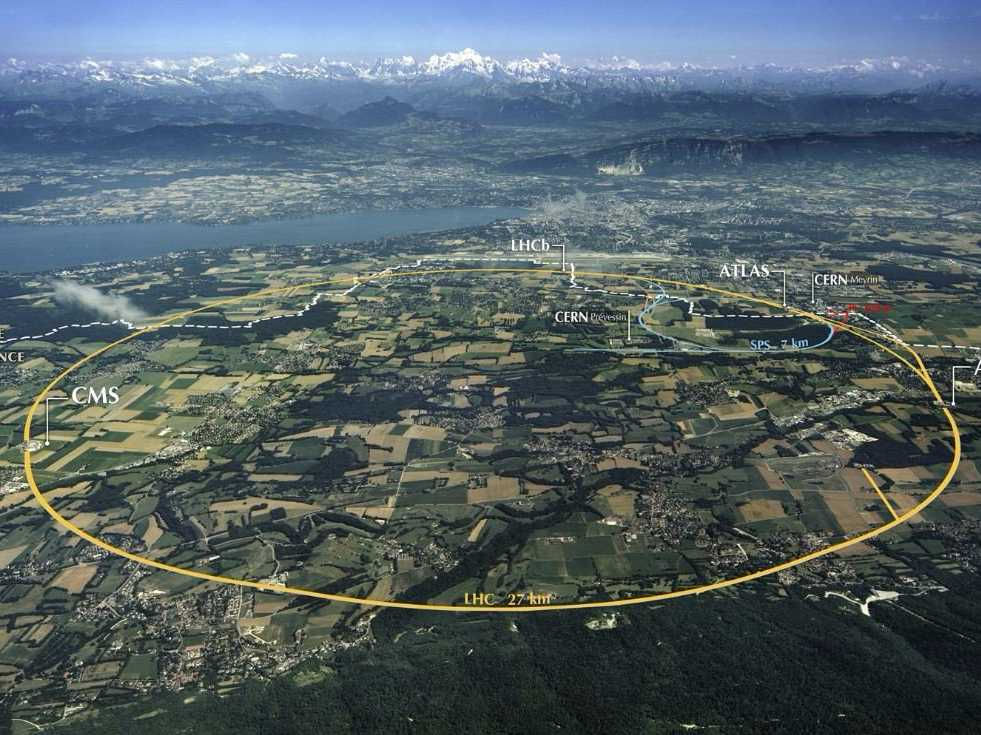
\includegraphics[width=\figwidth]{\figpath/CERN-LHC.jpg}
        \end{column}
    \end{columns}
\end{frame}

%%--------------------------------------------------------------------------------------------

\subsection*{Large Hadron Collider (LHC)}

%%--------------------------------------------------------------------------------------------

\frame{
    \frametitle{The Large Hadron Collider (LHC)}
    \vspace*{-0.24cm}
    \begin{columns}[T]
        \column{0.58\textwidth}
            \vspace*{0.6cm}
            \begin{block}{}
                \begin{itemize}
                    \item Proton-proton collider
                    \begin{itemize}
                        \item 27\unit{km} circumference
                        \item $\sim$100\unit{m} underground
                        \item Design center of mass energy of 14\TeV
                        \item Crossing rate 25\unit{ns}
                    \end{itemize}
                    \vspace*{0.2cm}
                    \item This analysis uses the full 2012 dataset
                    \begin{itemize}
                        \item \CM{8\tev}, 50\unit{ns}
                        \item $\int \mathcal{L}\sim$19.148 (19.279)\fbinv for electrons (muons)
                    \end{itemize}
                    \vspace*{0.2cm}
                    \item Two general purpose detectors (\textbf{CMS} \& ATLAS) and several other specialized experiments
                \end{itemize}
            \end{block}
        \column{0.4\textwidth}
            \hspace*{0.1cm}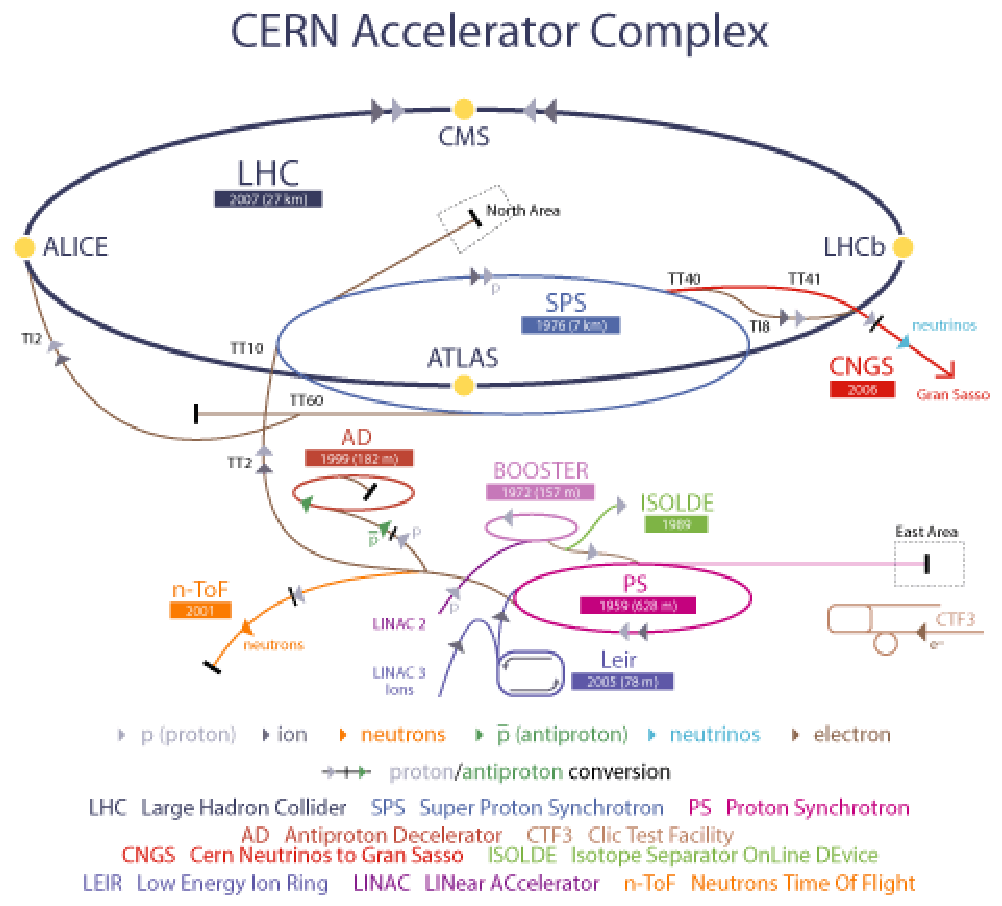
\includegraphics[width=\figwidth]{\figpath/AccComplex.pdf}\\
            \hspace*{0.1cm}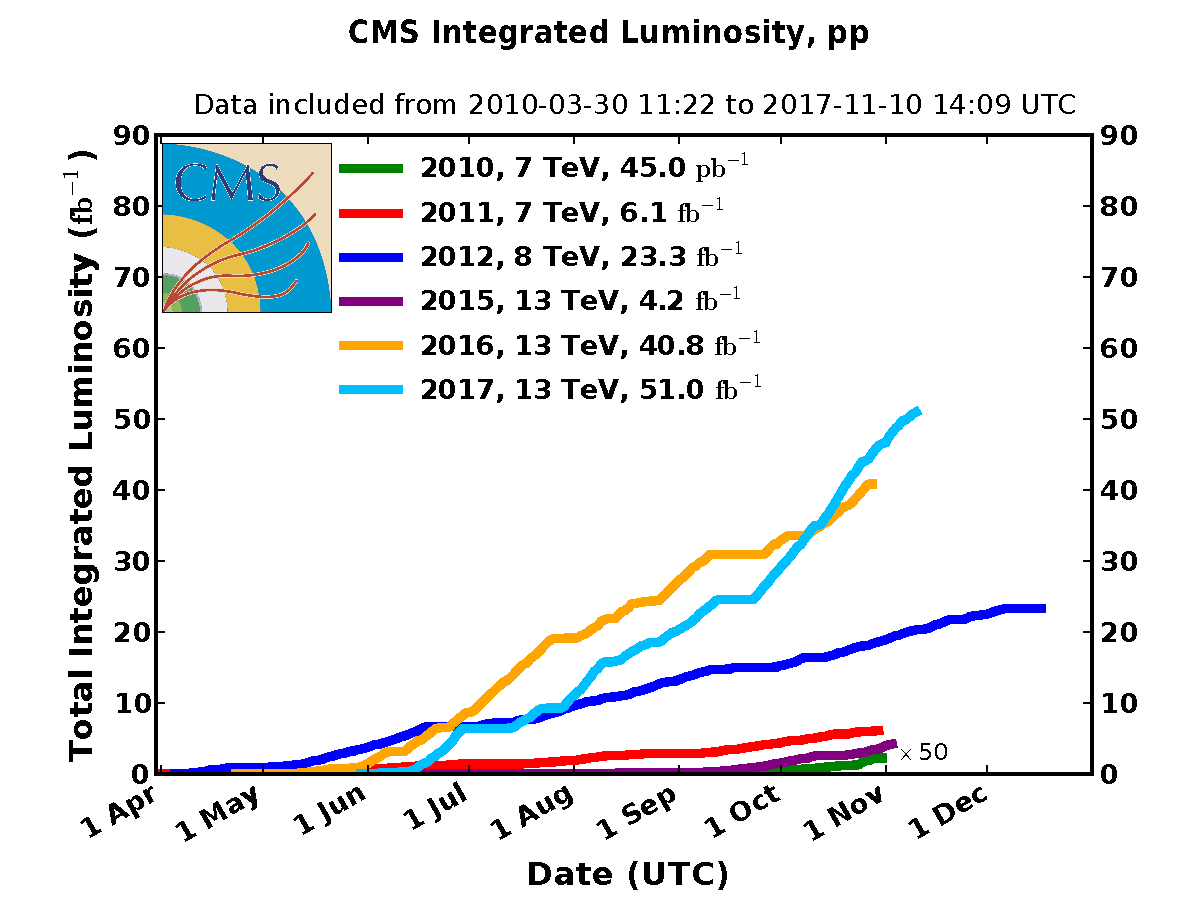
\includegraphics[width=\figwidth]{\figpath/int_lumi_cumulative_pp_2.pdf}
    \end{columns}
}

%%--------------------------------------------------------------------------------------------

\subsection*{Compact Muon Solenoid (CMS)}

%%--------------------------------------------------------------------------------------------

\frame{
    \frametitle{The Compact Muon Solenoid (CMS)}
    \vspace*{-0.24cm}
    \begin{block}{}
        \begin{itemize}
            \small
            \item Standard multipurpose detector, benefits from:
            \begin{itemize}
                \footnotesize
                \item High magnetic field
                \item High granularity tracker (lepton finding)
                \item Excellent electromagnetic calorimeter resolution
                \item Good particle identification due to the particle flow (PF) algorithm
            \end{itemize}            
        \end{itemize}
    \end{block}
    \begin{columns}[T]
        \begin{column}{0.65\textwidth}
            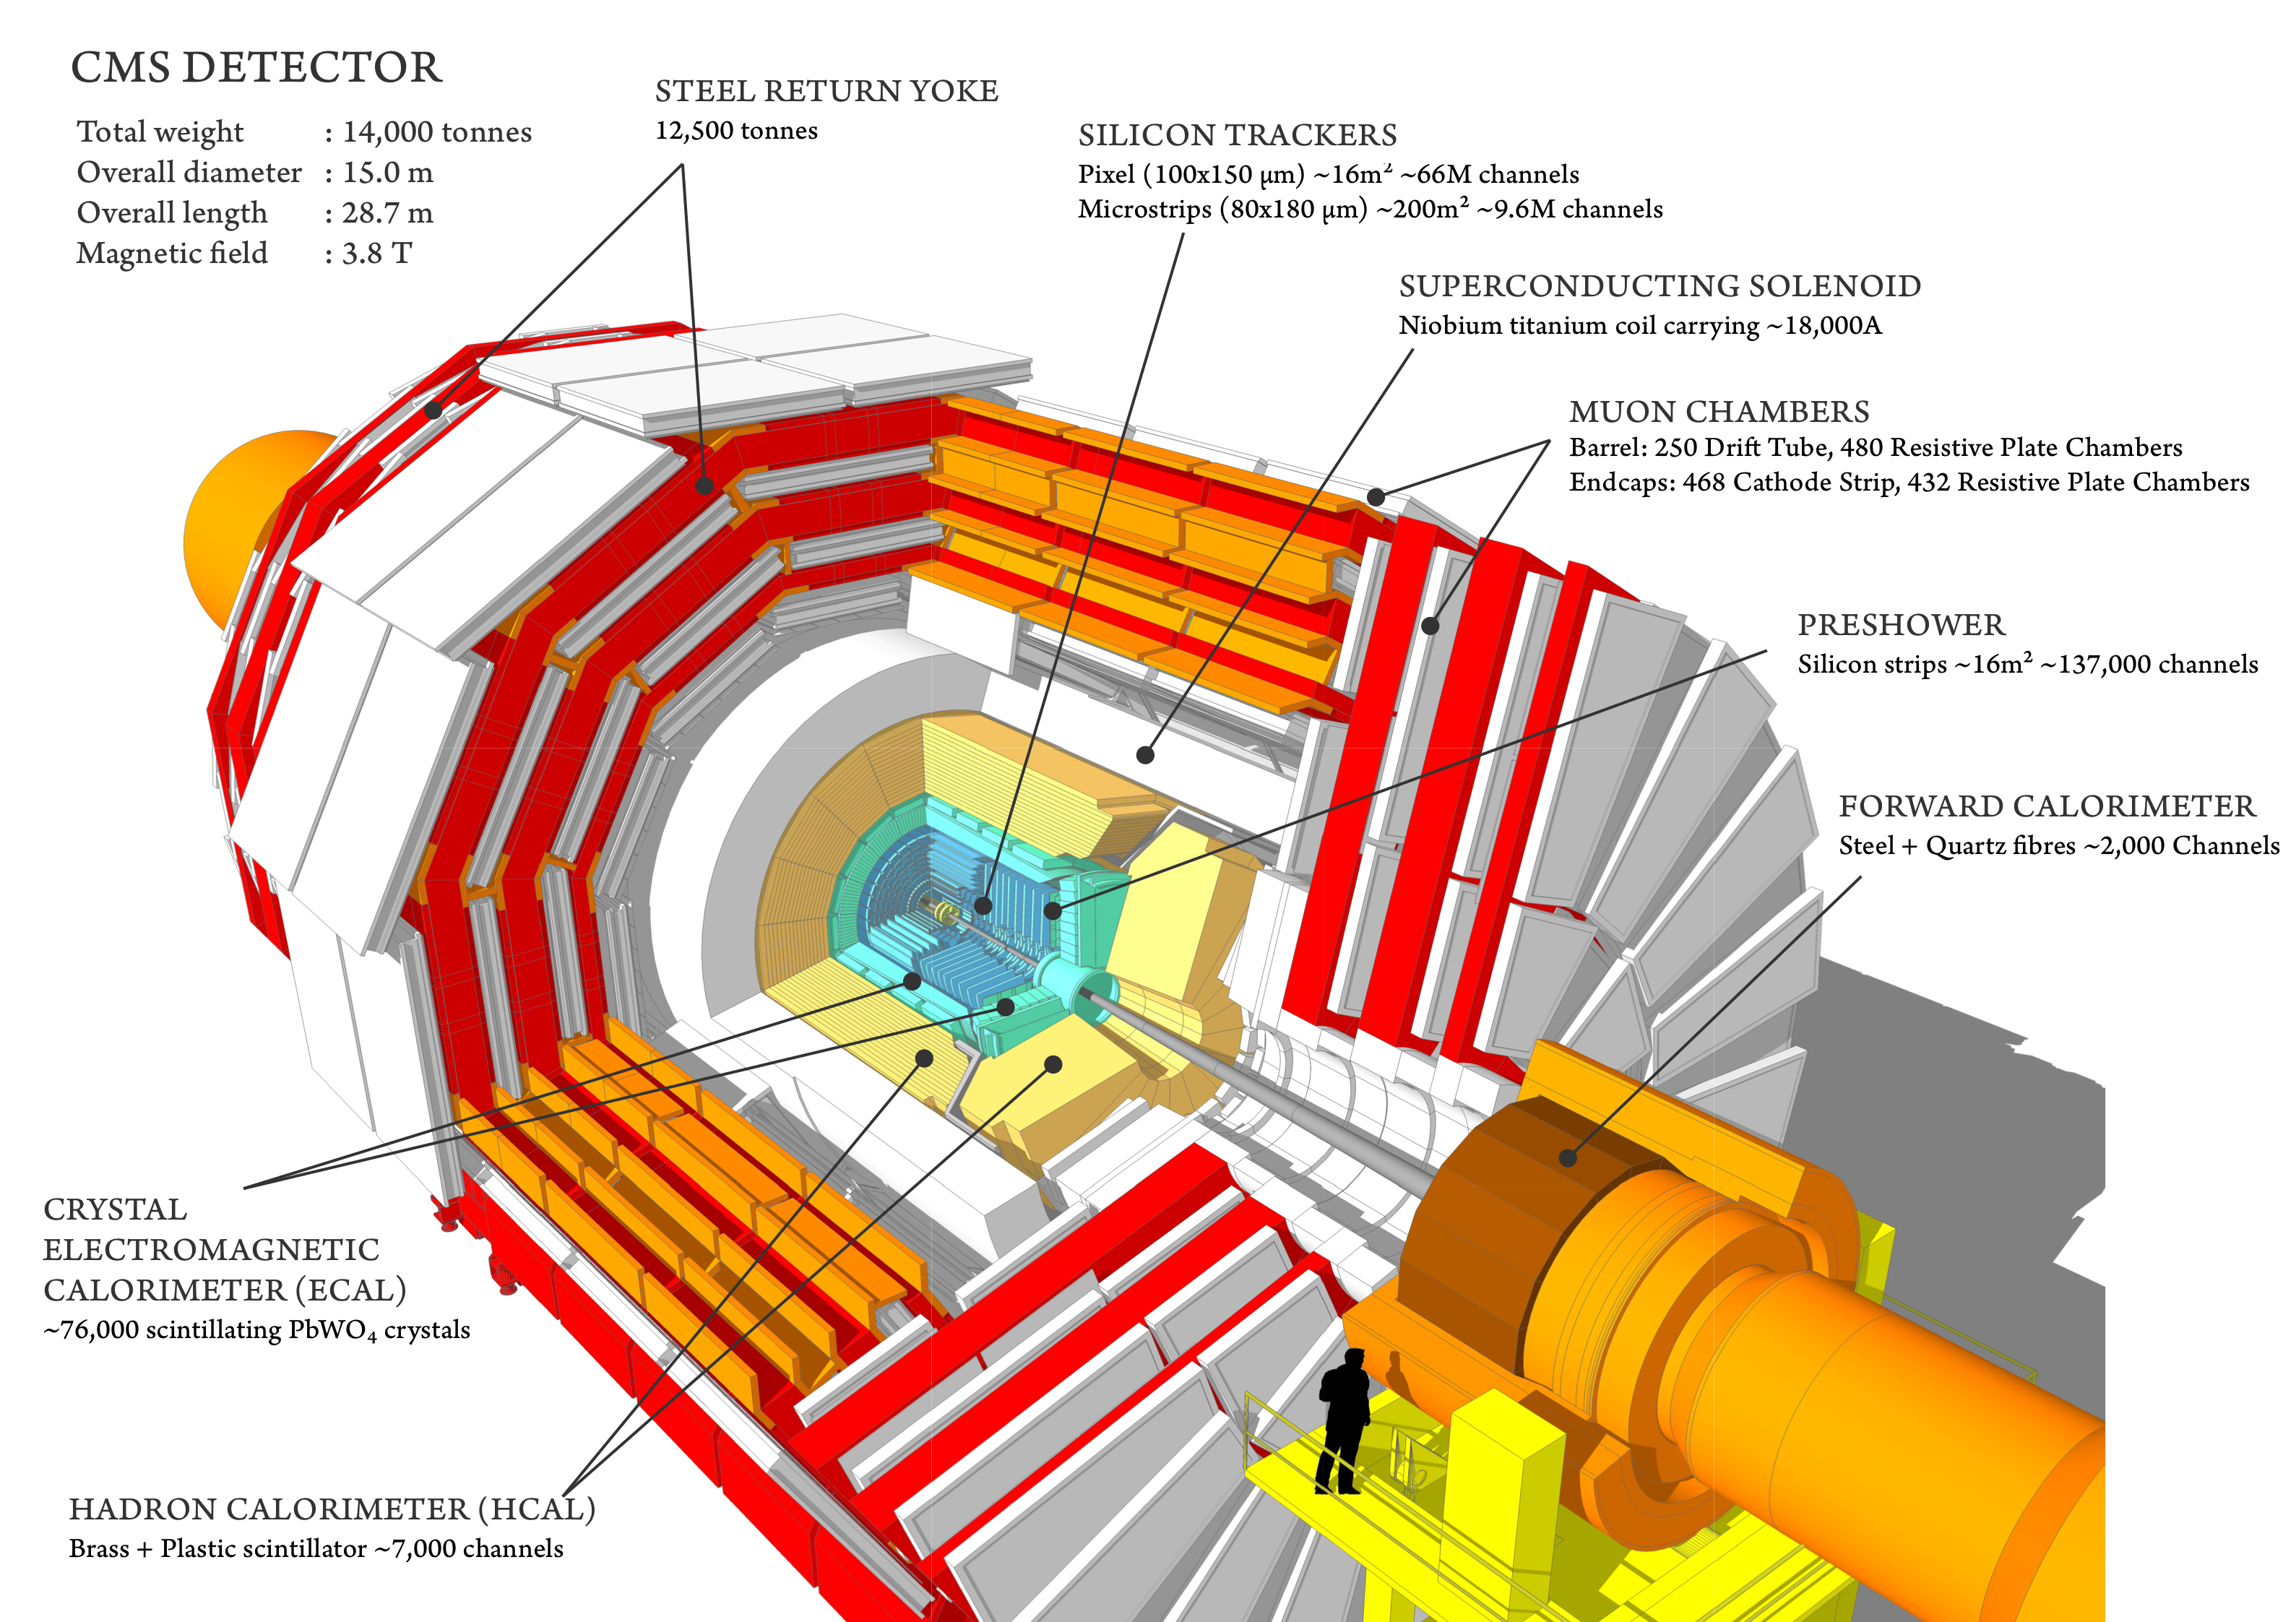
\includegraphics[width=\textwidth]{\figpath/cms.png}
        \end{column}
        \begin{column}{0.35\textwidth}
            \begin{figure}
                \centering
                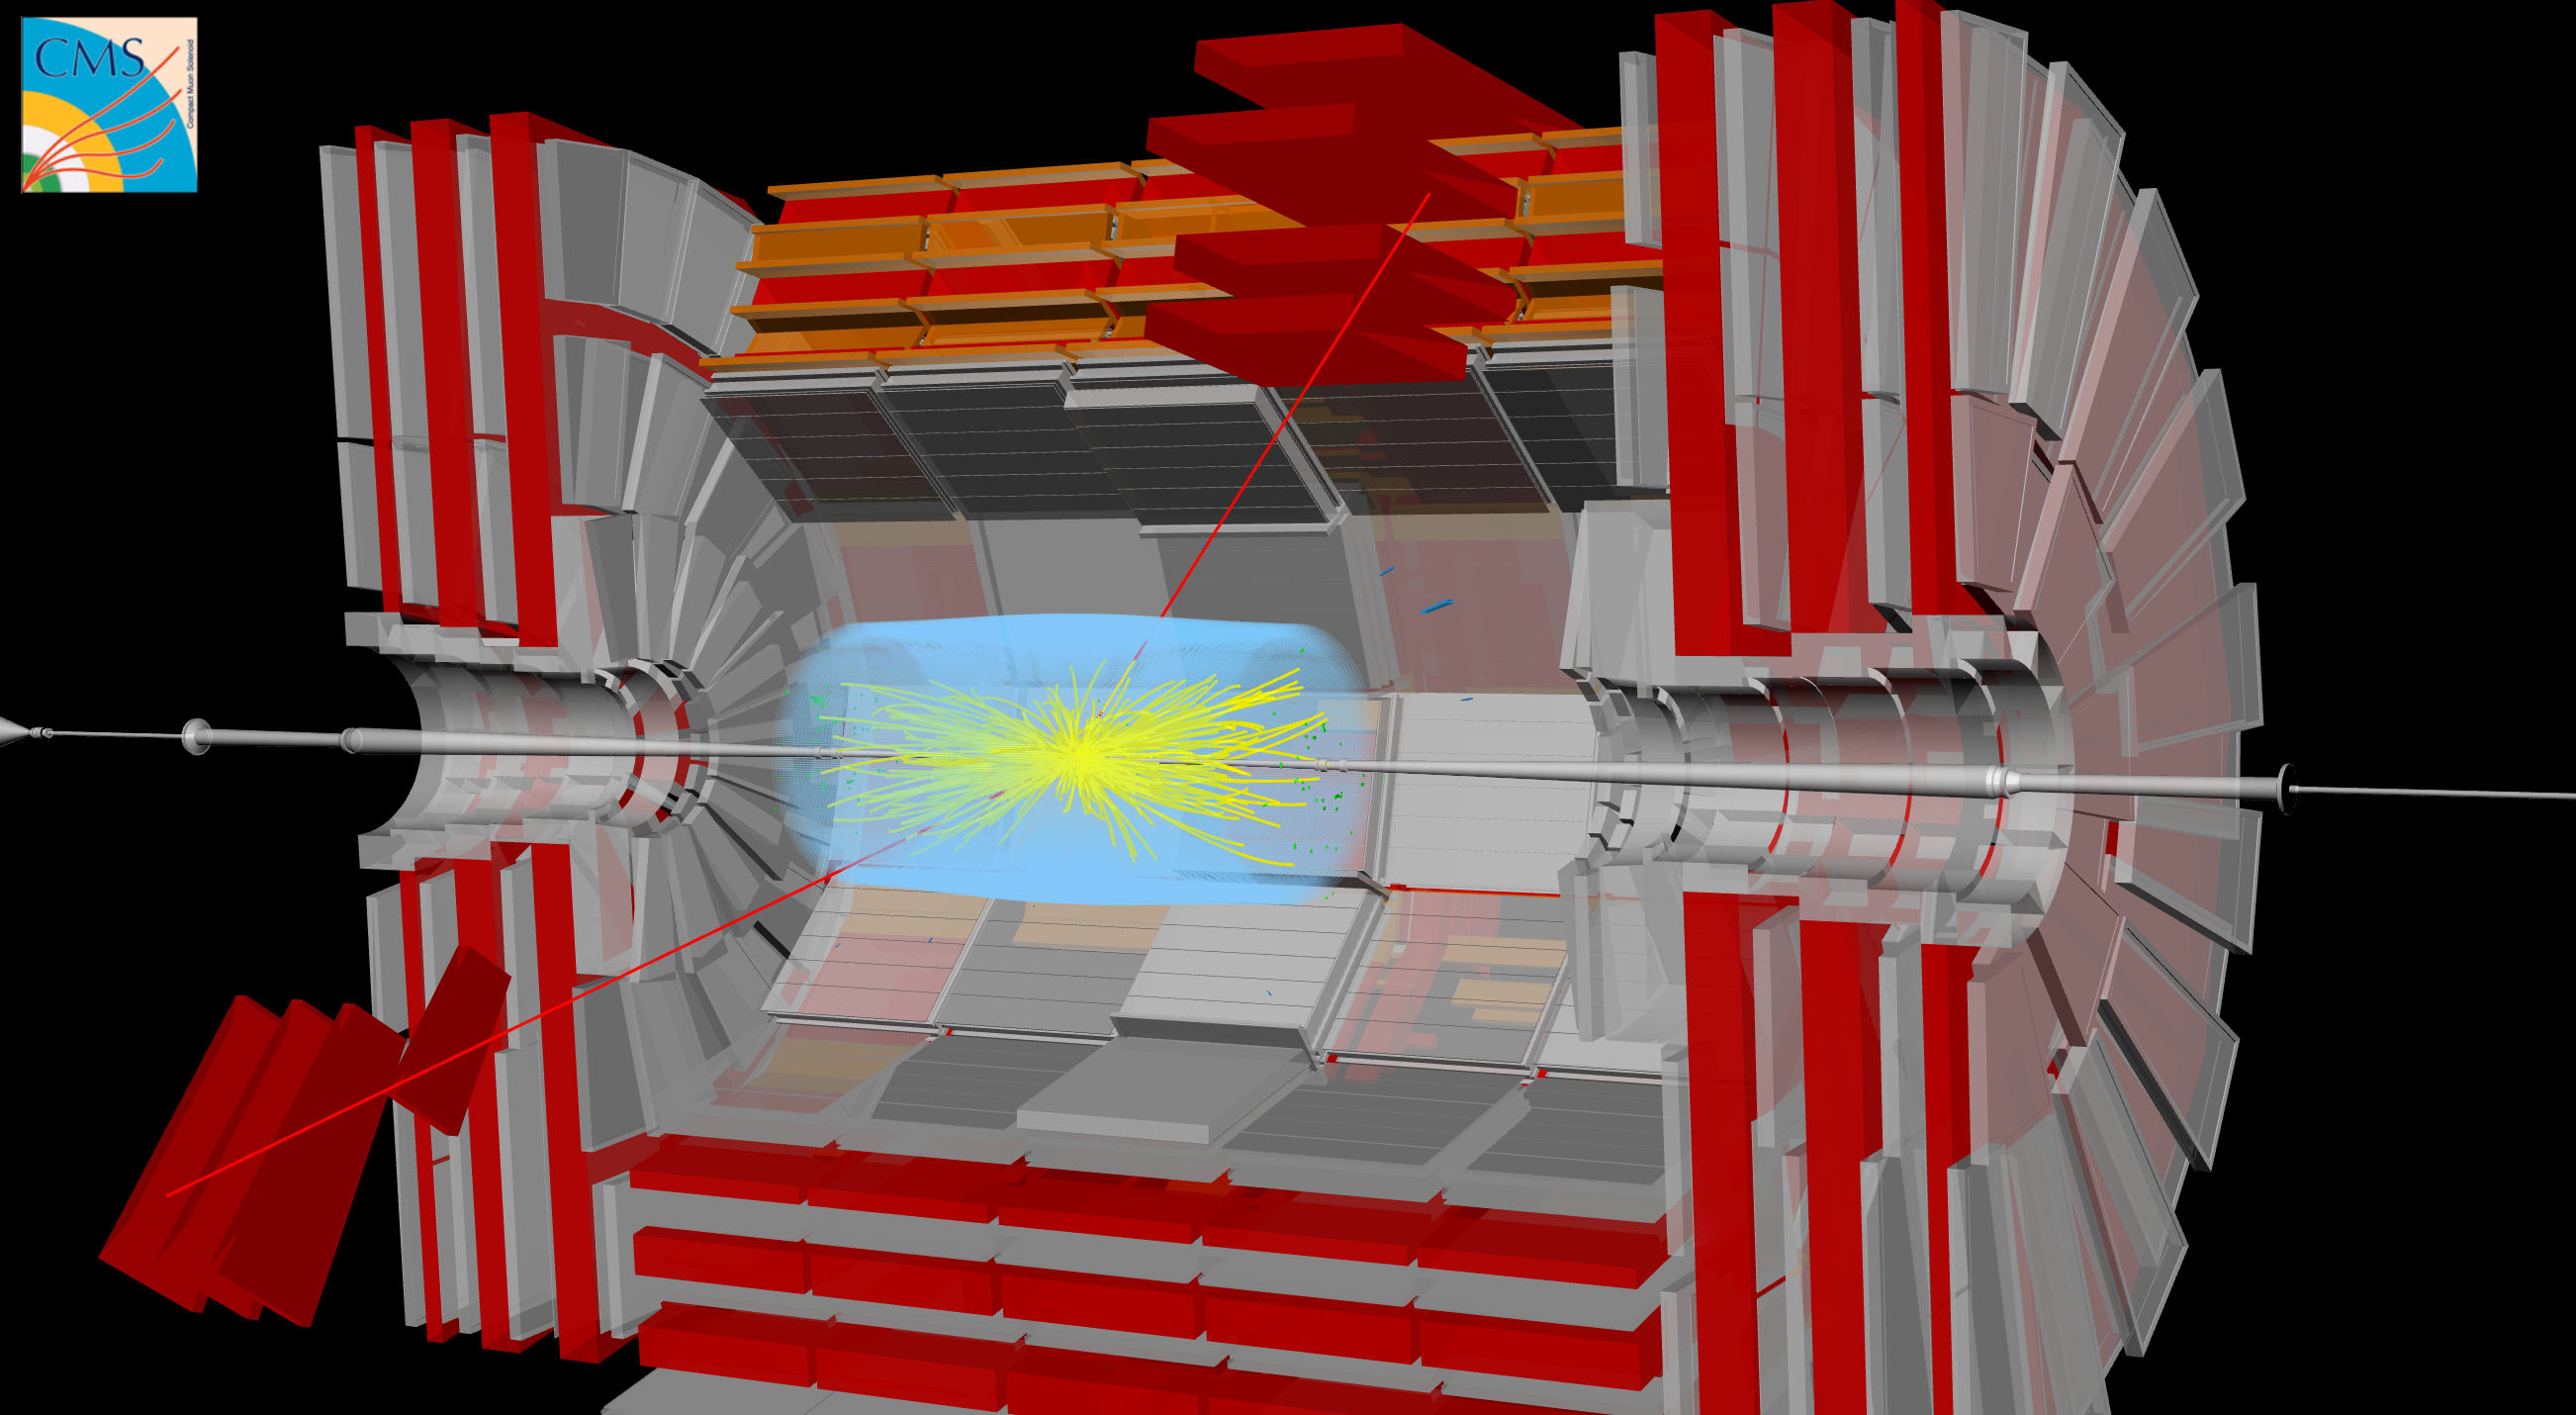
\includegraphics[width=\textwidth]{\figpath/dimuon_logo.png}
            \end{figure}
            \vfill
            \begin{figure}
                \centering
                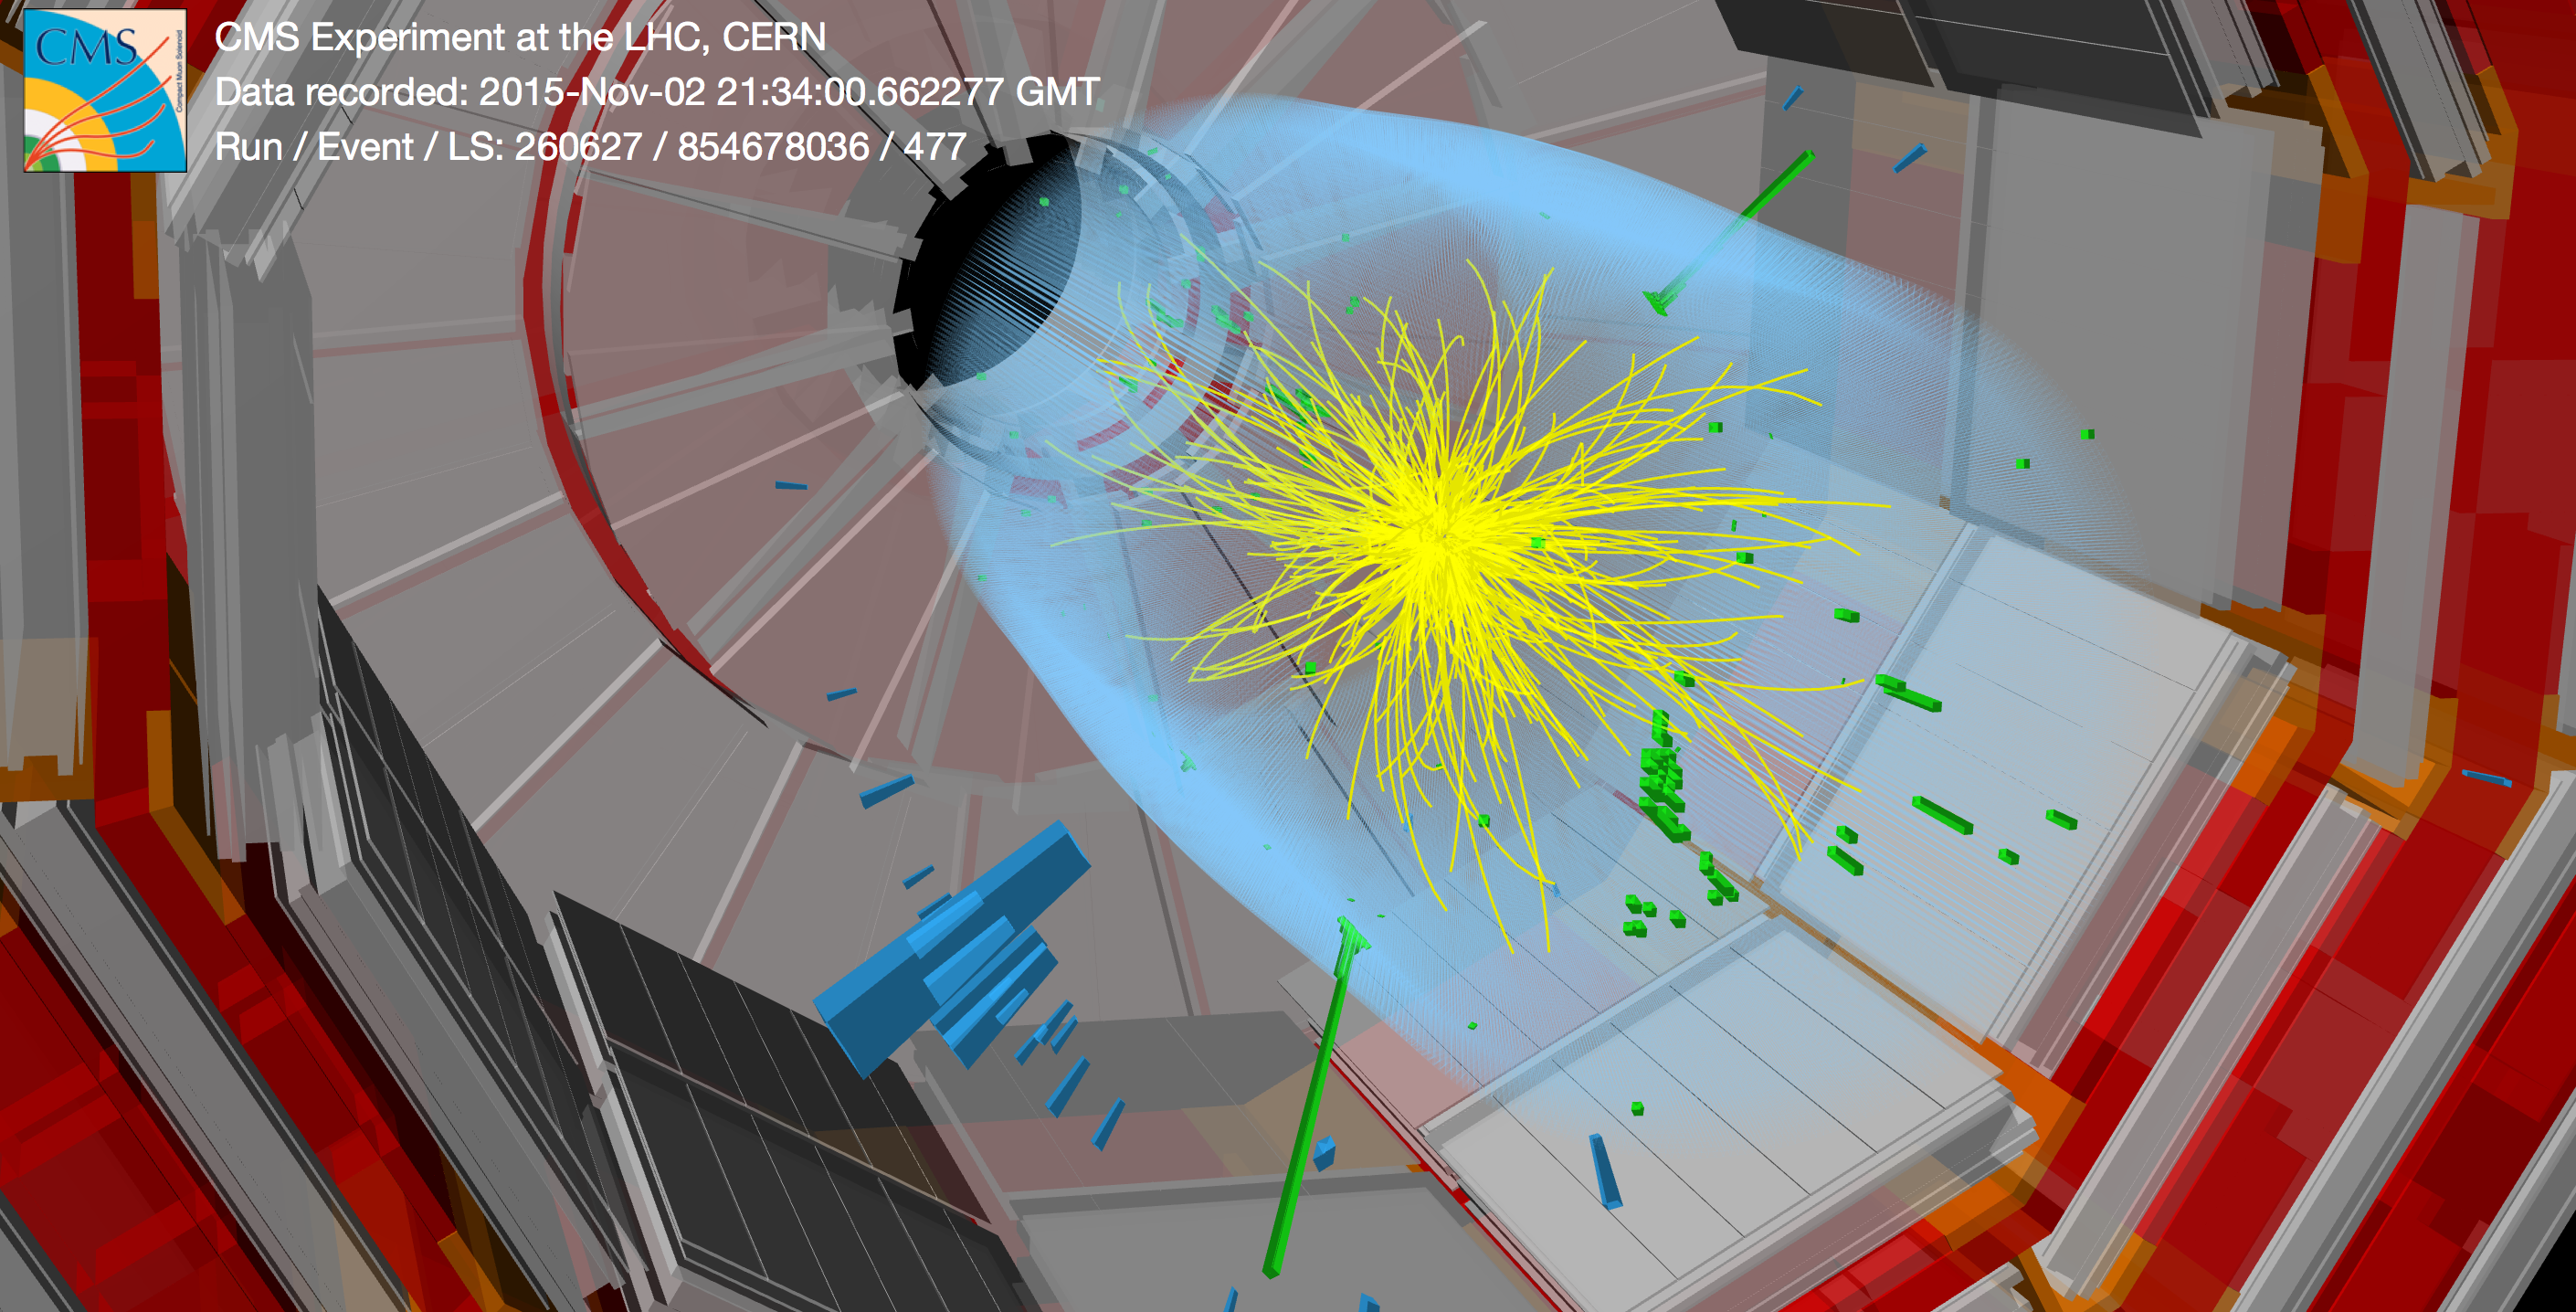
\includegraphics[width=\textwidth]{\figpath/diphoton_v2.png}
            \end{figure}
        \end{column}
    \end{columns}
}

\begin{frame}%<1>[label=frame:definitions]
    \setbeamercovered{transparent}
    \frametitle{Definitions}
    \vspace*{-0.24cm}
    \begin{block}{Coordinate System}
        \begin{columns}[T]
            \column{0.5\textwidth}
                \begin{itemize}
                    \scriptsize{
                      \item z-axis - Along the beam pipe
                      \item $\phi$ - The azimuthal angle
                      \item $\eta=-ln[tan(\frac{\theta}{2})]$ (called pseudorapidity)
                      \item $p_{T}$ - The transverse momentum (in the x-y plane)
                    }
                \end{itemize}
            \column{0.5\textwidth}
                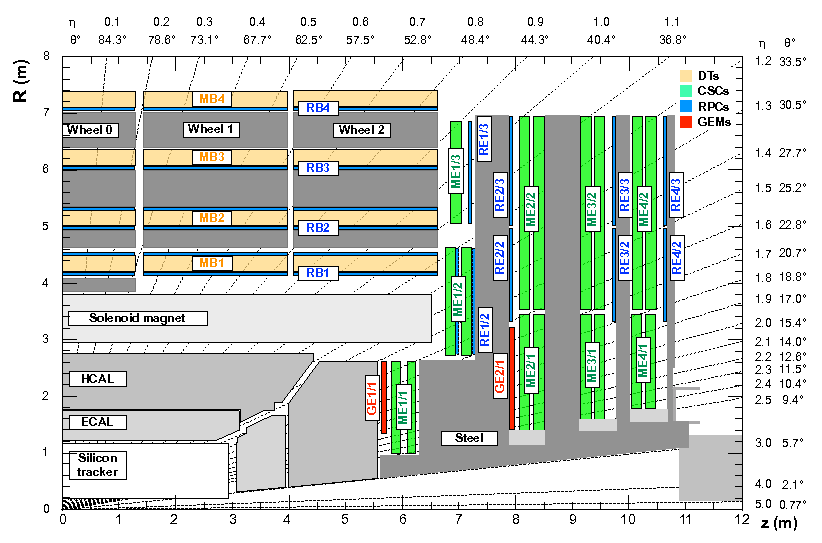
\includegraphics[width=0.53\textwidth]{\figpath/gem_sketch.png}
                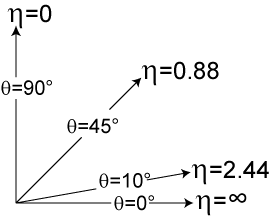
\includegraphics[width=0.45\textwidth]{\figpath/Pseudorapidity2.png}
        \end{columns}
    \end{block}
    \vspace*{-0.16cm}
    \begin{block}{Physics Objects}
        \begin{columns}[T]
            \column{0.45\textwidth}
                \begin{itemize}
                    \scriptsize{
                        \uncover<2->{\item Leptons {\color{gray}(Hadrons/Photons)}}
                        \uncover<3->{\item $\Em_{T}$ - Missing transverse energy
                        \begin{itemize}
                            \scriptsize{
                                \item Intrinsically from neutrinos
                                \item Indirectly from:
                                \begin{itemize}
                                    \scriptsize
                                    \item Jet Mismeasurements
                                    \item Detector Noise
                                    \item Pileup (multiple hard scatter interactions per bunch crossing)
                                \end{itemize}
                            }
                        \end{itemize}}
                        \uncover<4->{\item Jet - Collimated spray of particles
                        \begin{itemize}
                            \scriptsize{
                                \item Resulting from the hadronization of quarks and gluons
                            }
                        \end{itemize}}
                    }
                \end{itemize}
            \column{0.55\textwidth}
                \vspace*{-0.2cm}
                \begin{center}
                    \only<1-2>{\vspace*{0.25cm}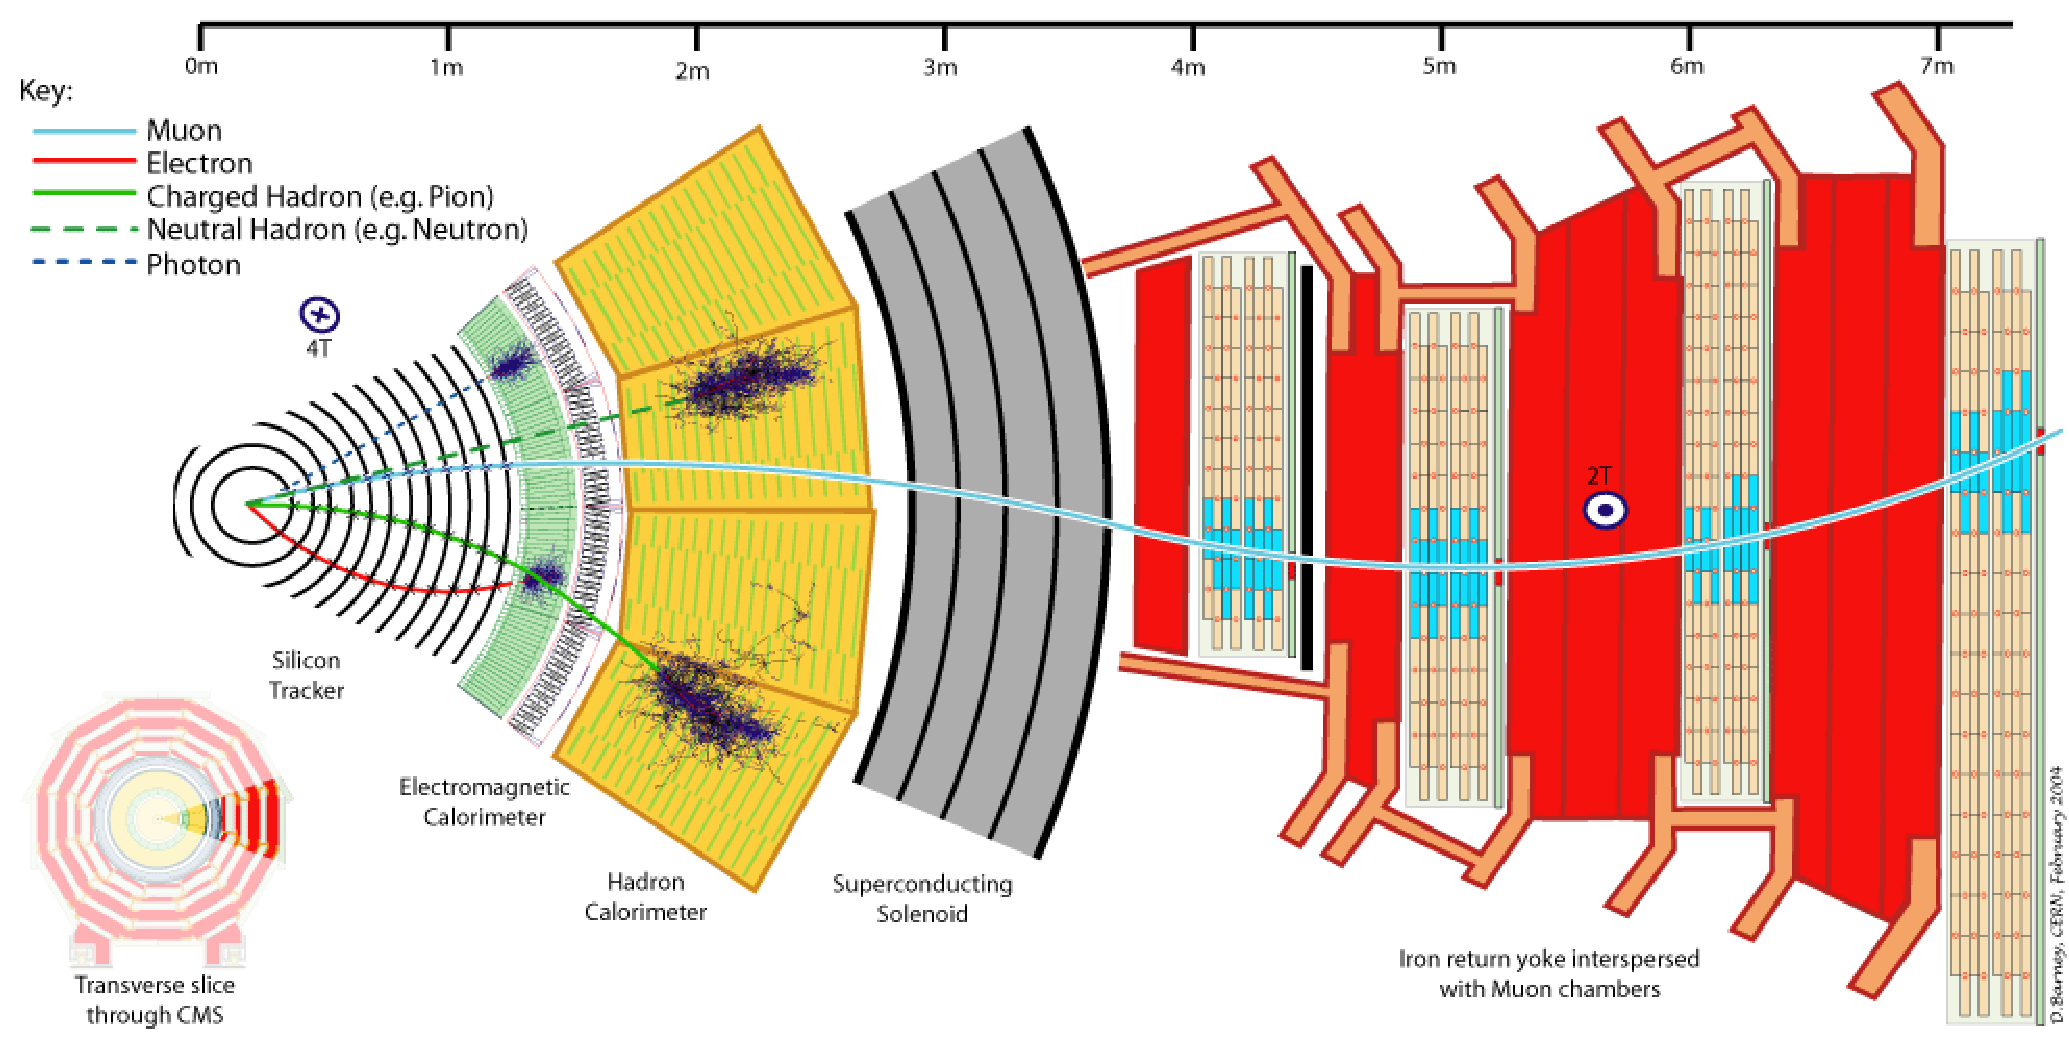
\includegraphics[width=\textwidth]{\figpath/CMS_Slice.pdf}}
                    %\only<3>{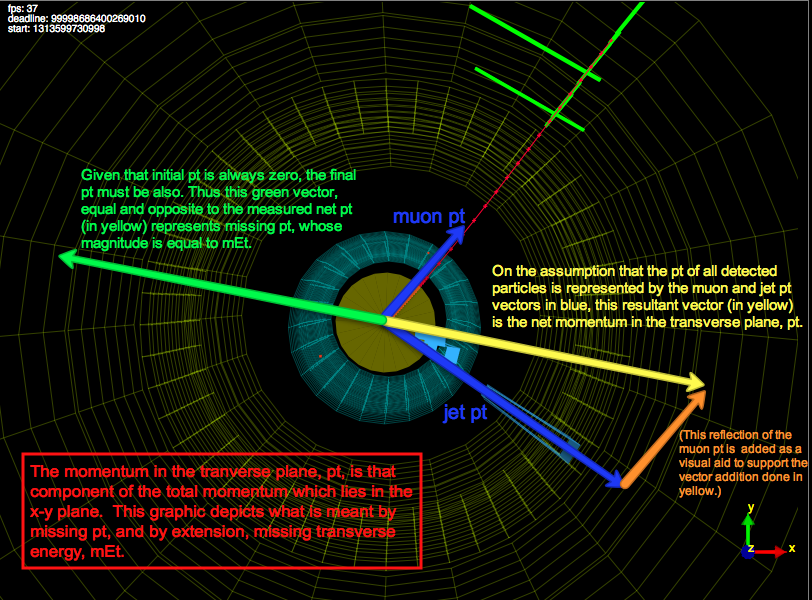
\includegraphics[width=0.8\textwidth]{\figpath/MEt.png}}
                    \only<3>{
                        \vspace*{-0.05cm}
                        \hspace*{0.95cm}\begin{tikzpicture}[scale=0.9]
                            \node[inner sep=0pt] {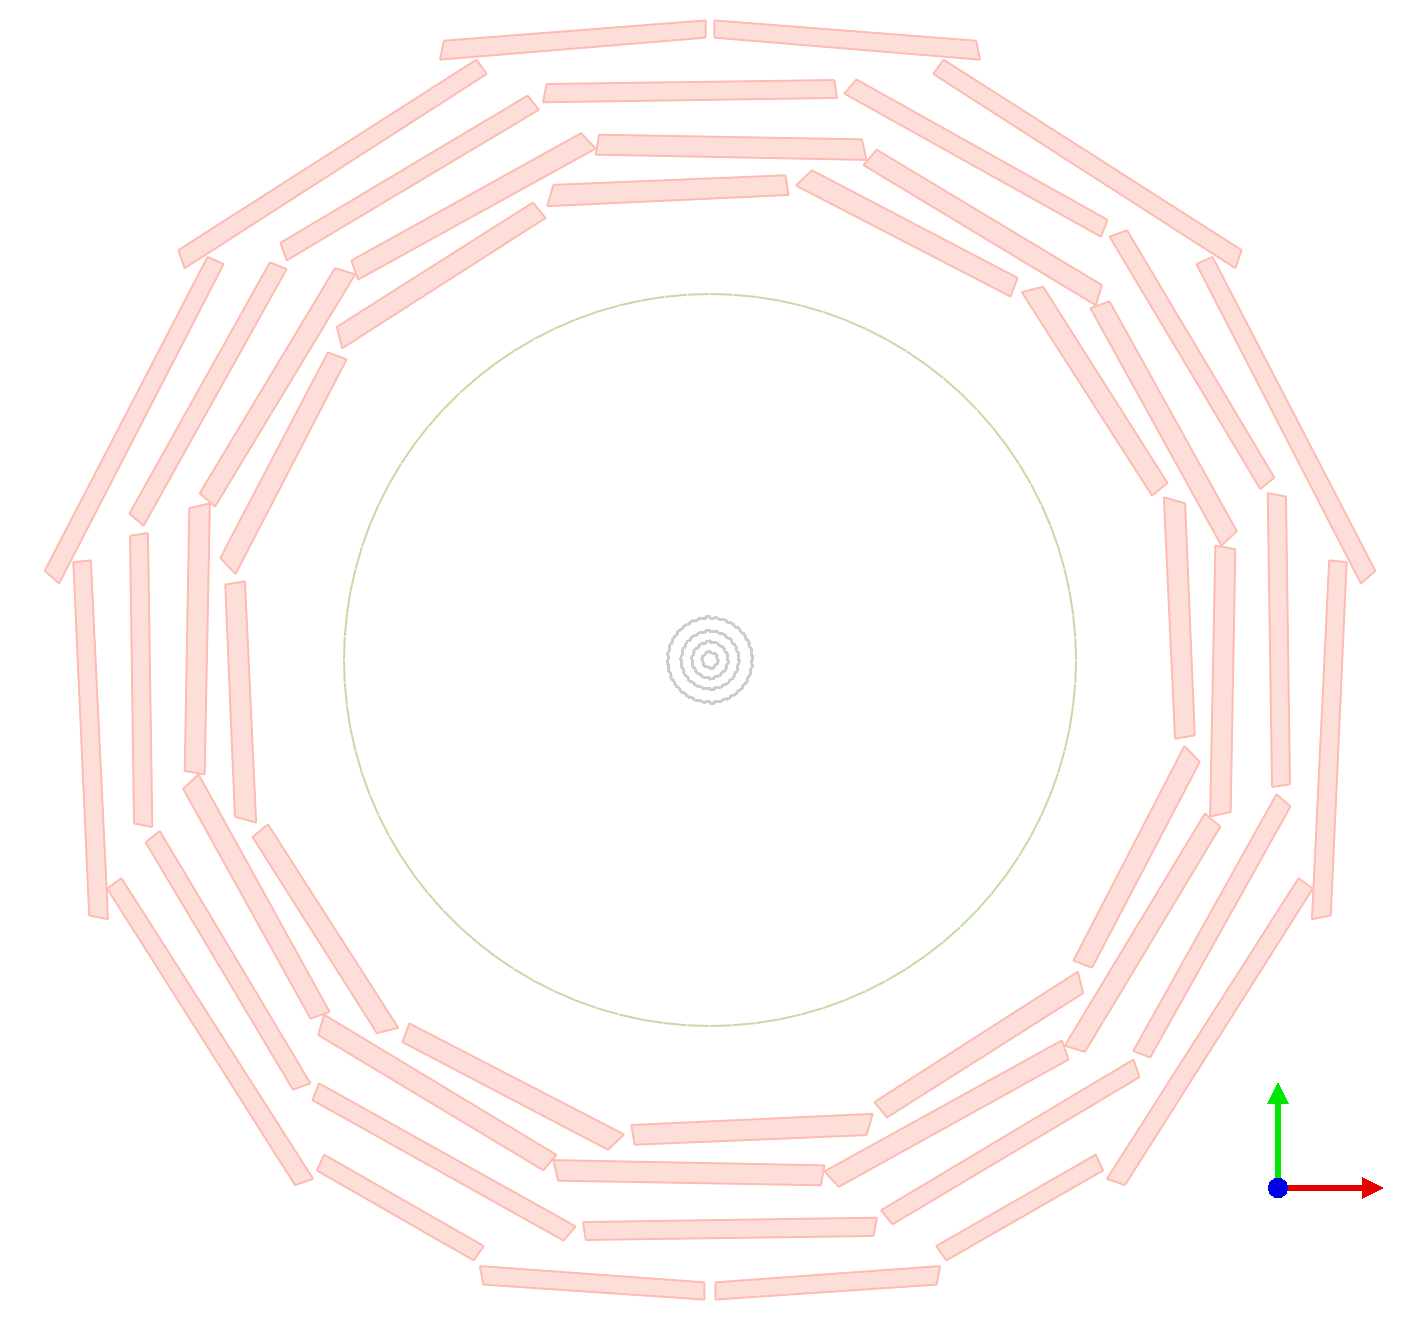
\includegraphics[width=0.65\textwidth]{\figpath/CMSWireframe_compressed.png}};
                            \draw[blue, thick, arrow] (0.0,0.0) -- (0.6,0.6) node[xshift=-0.8cm] {\footnotesize muon $p_{T}$};
                            \draw[blue, thick, arrow] (0.0,0.0) -- (1.4,-1.0) node[midway,left] {\footnotesize jet $p_{T}$};
                            \draw[orange, thick, arrow] (1.4,-1.0) -- (2.0,-0.4) node[midway,right, xshift=0.22cm, yshift=-0.1cm, text width=1.5cm] {\footnotesize shifted muon $p_{T}$};
                            \draw[Goldenrod, thick, arrow] (0.0,0.0) -- (2.0,-0.4) node[midway,xshift=0.25cm, yshift=0.25cm] {\footnotesize $\sum_{\text{\scriptsize objects}} p_{T}$};
                            \draw[green, thick, arrow] (0.0,0.0) -- (-2.0,0.4) node[xshift=0.5cm,yshift=0.25cm] {\footnotesize \VETslash};
                            \node[outer sep=1pt, text=Goldenrod] at (2.4,-1.8) {\tiny x};
                            \node[outer sep=1pt, text=Goldenrod] at (1.95,-1.35) {\tiny y};
                            \node[outer sep=1pt, text=Goldenrod] at (1.95,-1.8) {\tiny z};
                        \end{tikzpicture}
                    }
                    \only<4>{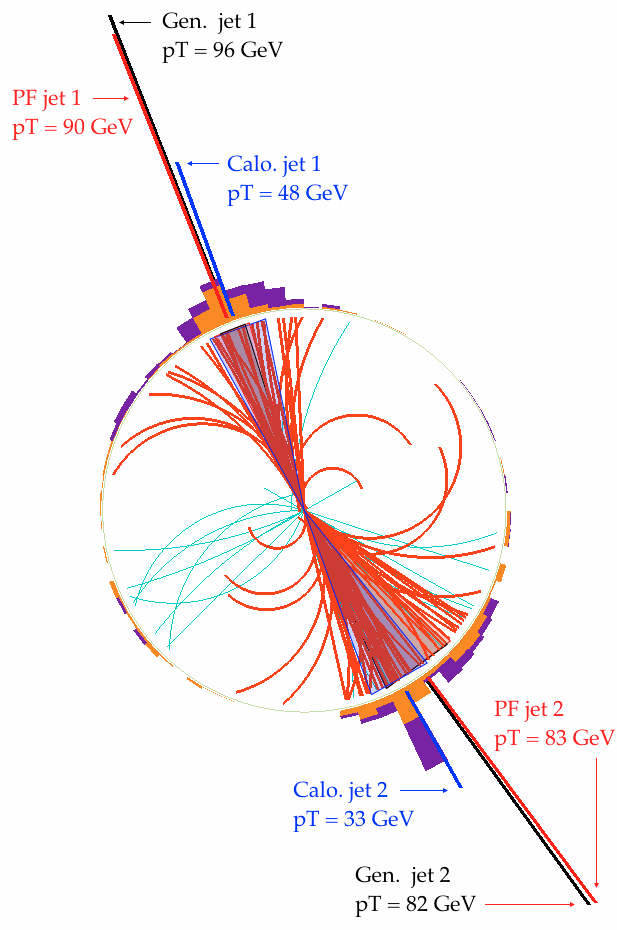
\includegraphics[width=0.4\textwidth]{\figpath/display_xy_annotated.png}}
                \end{center}
        \end{columns}
    \end{block}
\end{frame}
%\againframe<2>{frame:definitions}
%\againframe<3>{frame:definitions}
%\againframe<4>{frame:definitions}

\addtocontents{toc}{\vskip 0.5cm}
\section[Evt. Sel.]{Event Selection}
\label{sec:event_selection}
%!TEX root = ../DissertationDefensePresentation.tex

{
\usebackgroundtemplate{
  
\begin{tikzpicture}
    \path [outer color = white, inner color = gray!85]
      (0,0) rectangle (\paperwidth,\paperheight);
  \end{tikzpicture}}
\begin{frame}
    \begin{textblock}{1.0}(0.0,0.75)
        \begin{center}
            \Huge
            \HWWlvjj Analysis Details\\
        \end{center}
    \end{textblock}
\end{frame}
}

%%--------------------------------------------------------------------------------------------

\subsection*{Signal}

%%--------------------------------------------------------------------------------------------

\begin{frame}%<1>[label=frame:event_signature]
	\setlength{\leftmargini}{0.5cm}
	\setlength{\leftmarginii}{0.5cm}
	\setlength{\leftmarginiii}{0.5cm}
	\tikzstyle{na} = [baseline=-.5ex]
	\frametitle{Event Signature}
	\vspace*{-0.24cm}
	\begin{columns}[T]
		\begin{column}{0.5\textwidth}
			\vspace*{-0.25cm}
			\begin{block}{}
				\begin{itemize}
					\item Need a sample enriched in \HWW with a semi-leptonic signature:
					\begin{itemize}
						\item<2-> \textbf{Exactly 1 electron or muon} passing{\tikz[remember picture]{\node[coordinate] (s-lepton) {};}} the trigger and quality criteria
						\begin{itemize}
							\item<2-> $p_{T}>$30 (25)\gev for electrons (muons)
							\item<2-> No additional ``loose'' leptons
						\end{itemize}
						\item<3-> \textbf{At least 2 jets} passing the quality{\tikz[remember picture]{\node[coordinate] (s-jet) {};}} requirements
						\begin{itemize}
							\item<3-> Anti-k\textsubscript{T} PF$+$CHS, R$=$0.5
							\item<3-> (Sub-)Leading jet $p_{T}>$30 (25)\gev
						\end{itemize}
						\item<4-> \textbf{Must contain \ETslash$>$25\gev}{\tikz[remember picture]{\node[coordinate] (s-met) {};}}
						\begin{itemize}
							\item<4-> Removes some of the QCD background
						\end{itemize}
						\item<5-> \textbf{b-jet veto}{\tikz[remember picture]{\node[coordinate] (s-bjet) {};}}
						\begin{itemize}
							\item Removes a large portion of \ttbar events
						\end{itemize}
					\end{itemize}
					\item<6-> Details of the \HWWlvjj event selection criteria are discussed in the backup slides
				\end{itemize}
			\end{block}
		\end{column}
		\begin{column}{0.02\textwidth}
		\end{column}
		\begin{column}{0.445\textwidth}
			\only<1-4>{\vspace*{2cm}}
			\only<5-6>{\vspace*{1.5cm}}
			\begin{tikzpicture}[remember picture]
				% Put the graphic inside a node. This makes it easy to place the
				% graphic and to draw on top of it. 
				% The above right option is used to place the lower left corner
				% of the image at the (0,0) coordinate. 
				\only<1-4>{\node [inner sep=0pt,above right] {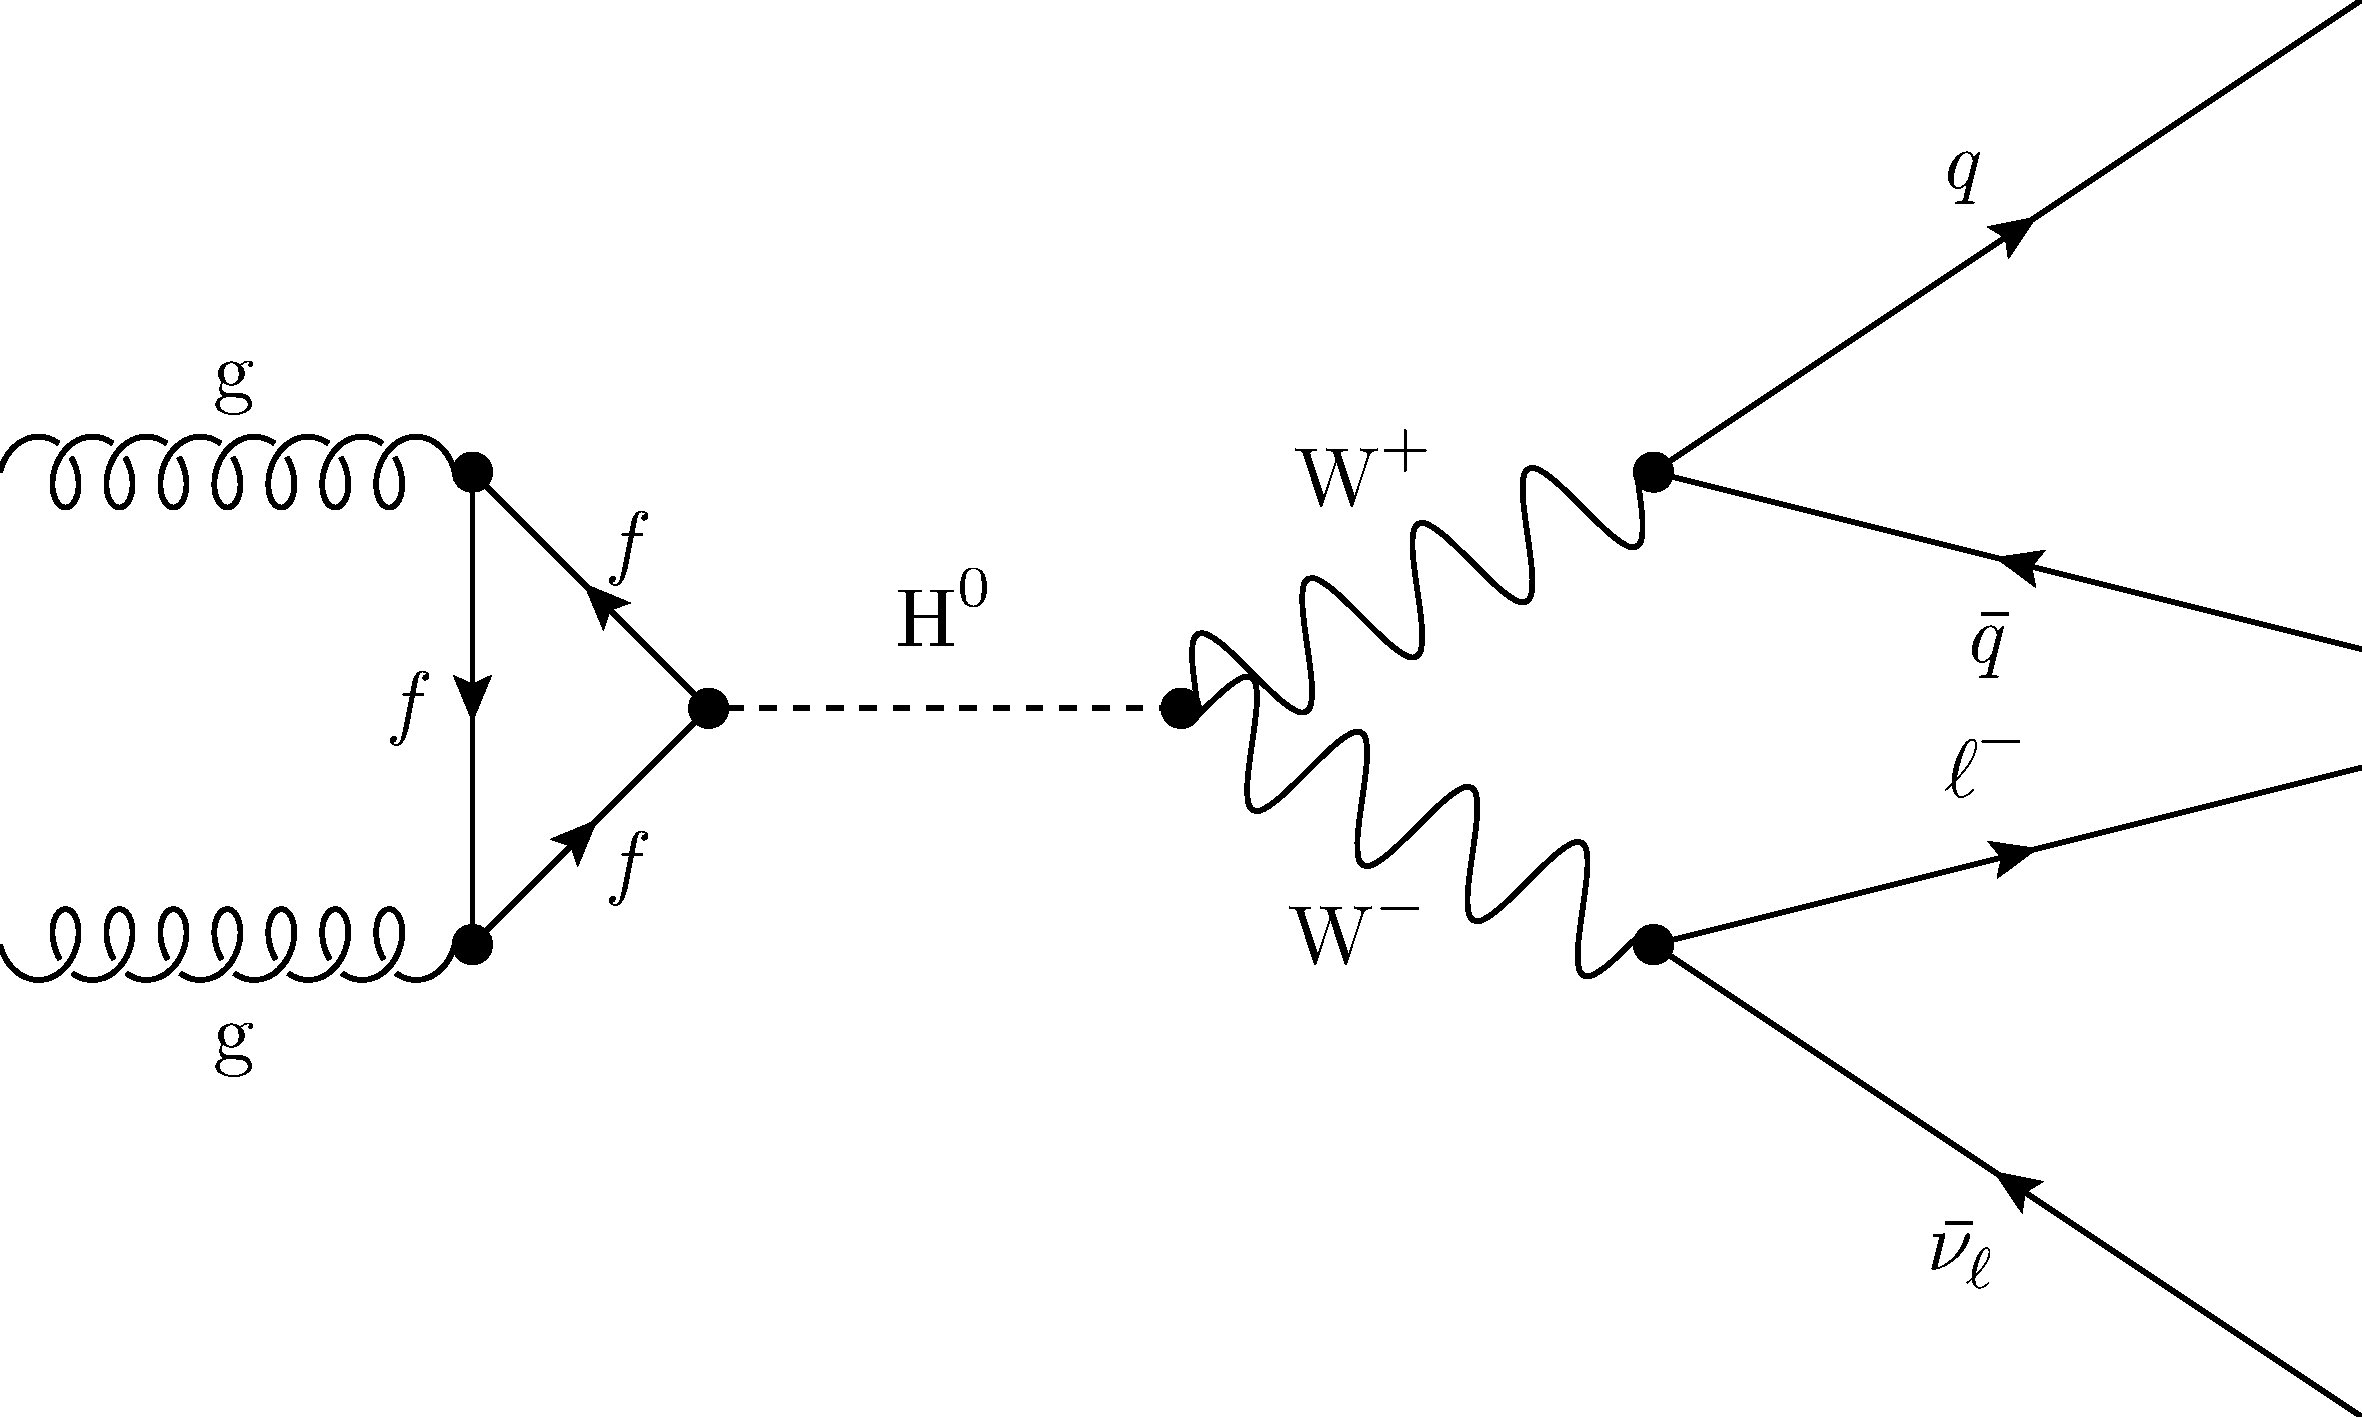
\includegraphics[width=\textwidth]{\figpath/FeynmanDiagrams/ggH_WW_lvjj.pdf}};}
				\only<5->{\node [inner sep=0pt,above right] {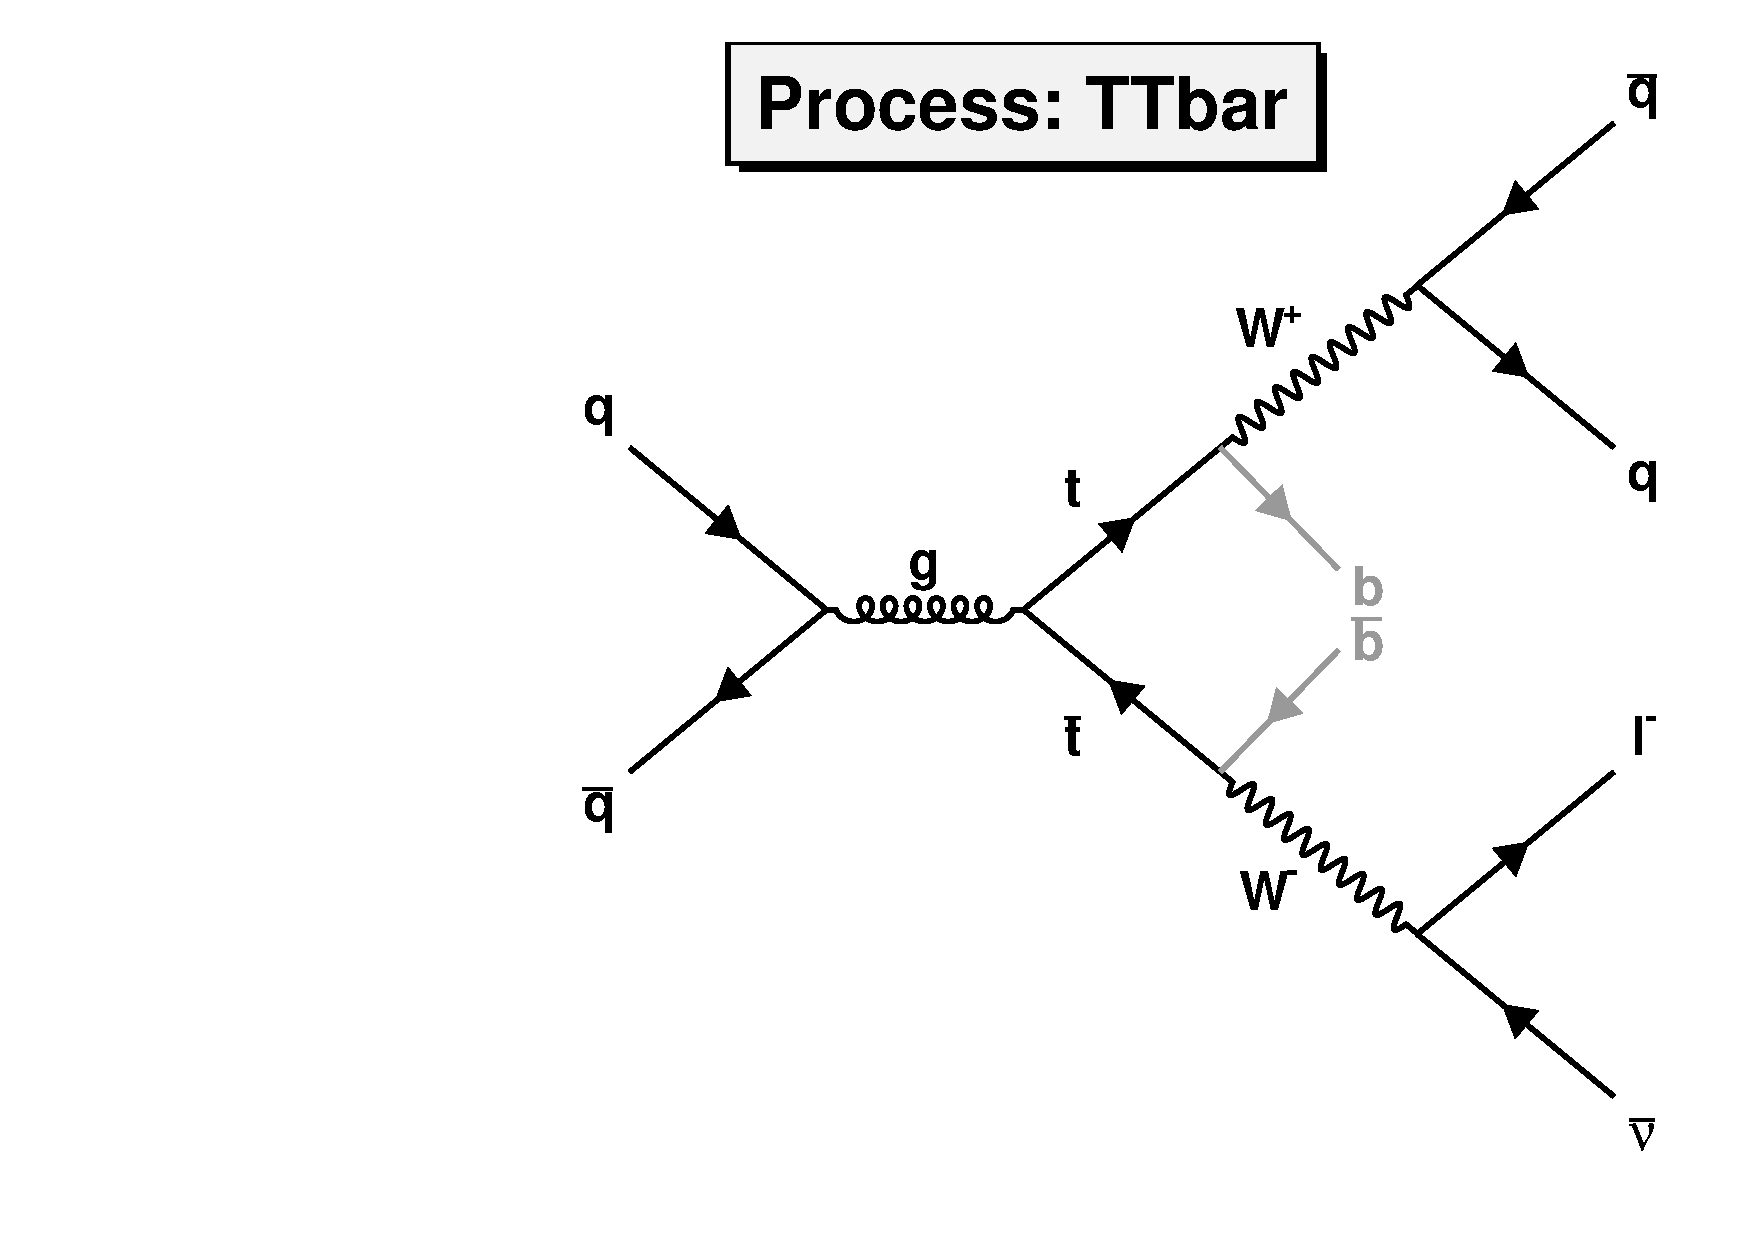
\includegraphics[width=\textwidth]{\figpath/FeynmanDiagrams/TTbar.pdf}};}
				%\only<6->{
				%	\node[rectangle, rounded corners, draw=red, very thick, anchor=base] (Irreducible) at (0,4) {%
				%		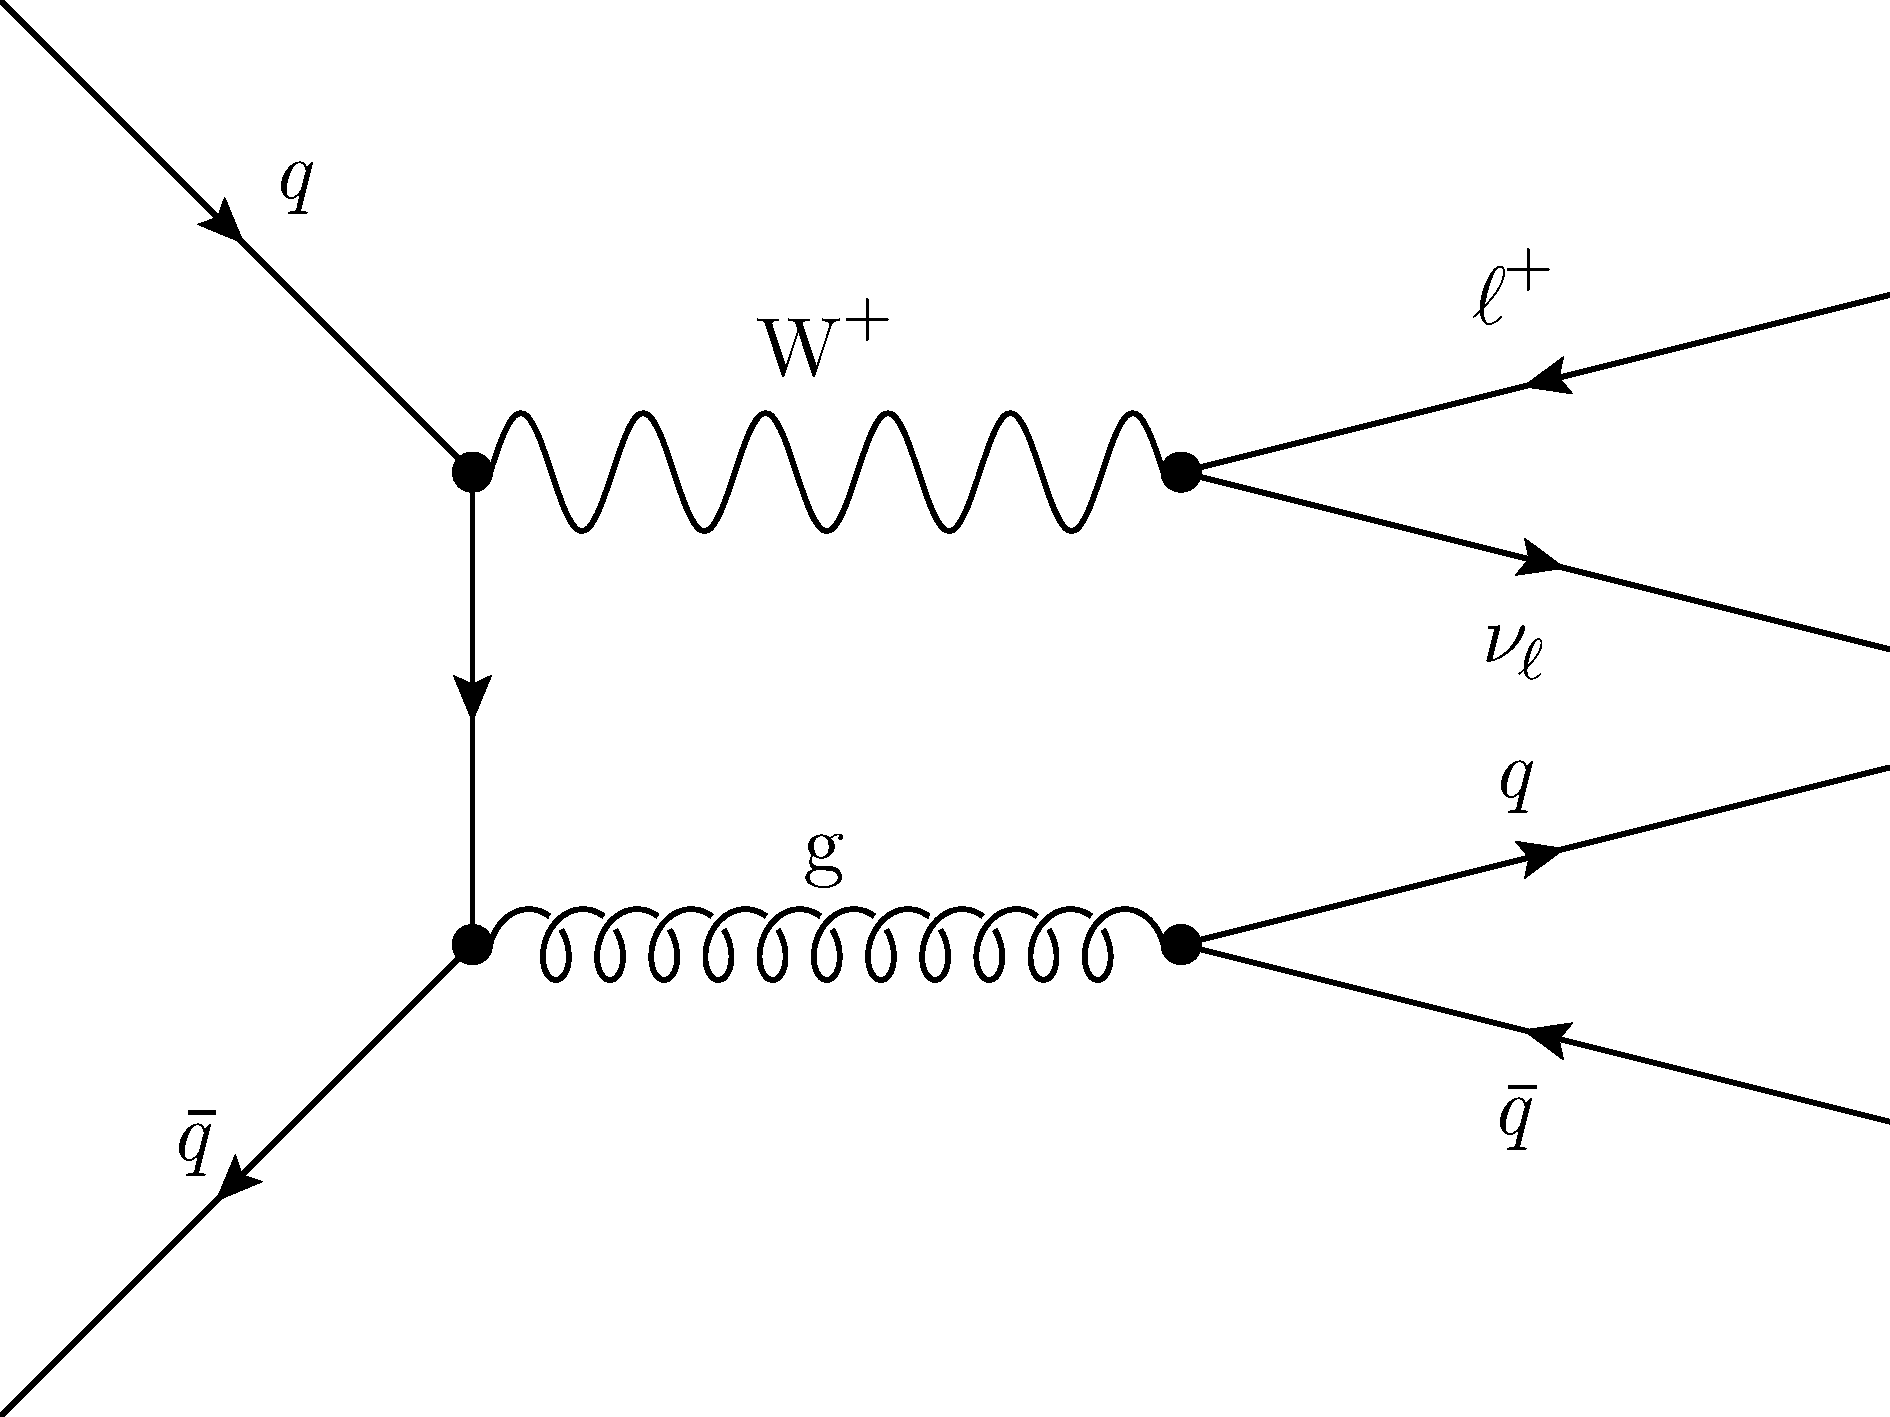
\includegraphics[width=0.48\textwidth]{\figpath/FeynmanDiagrams/WJets.pdf}
				%		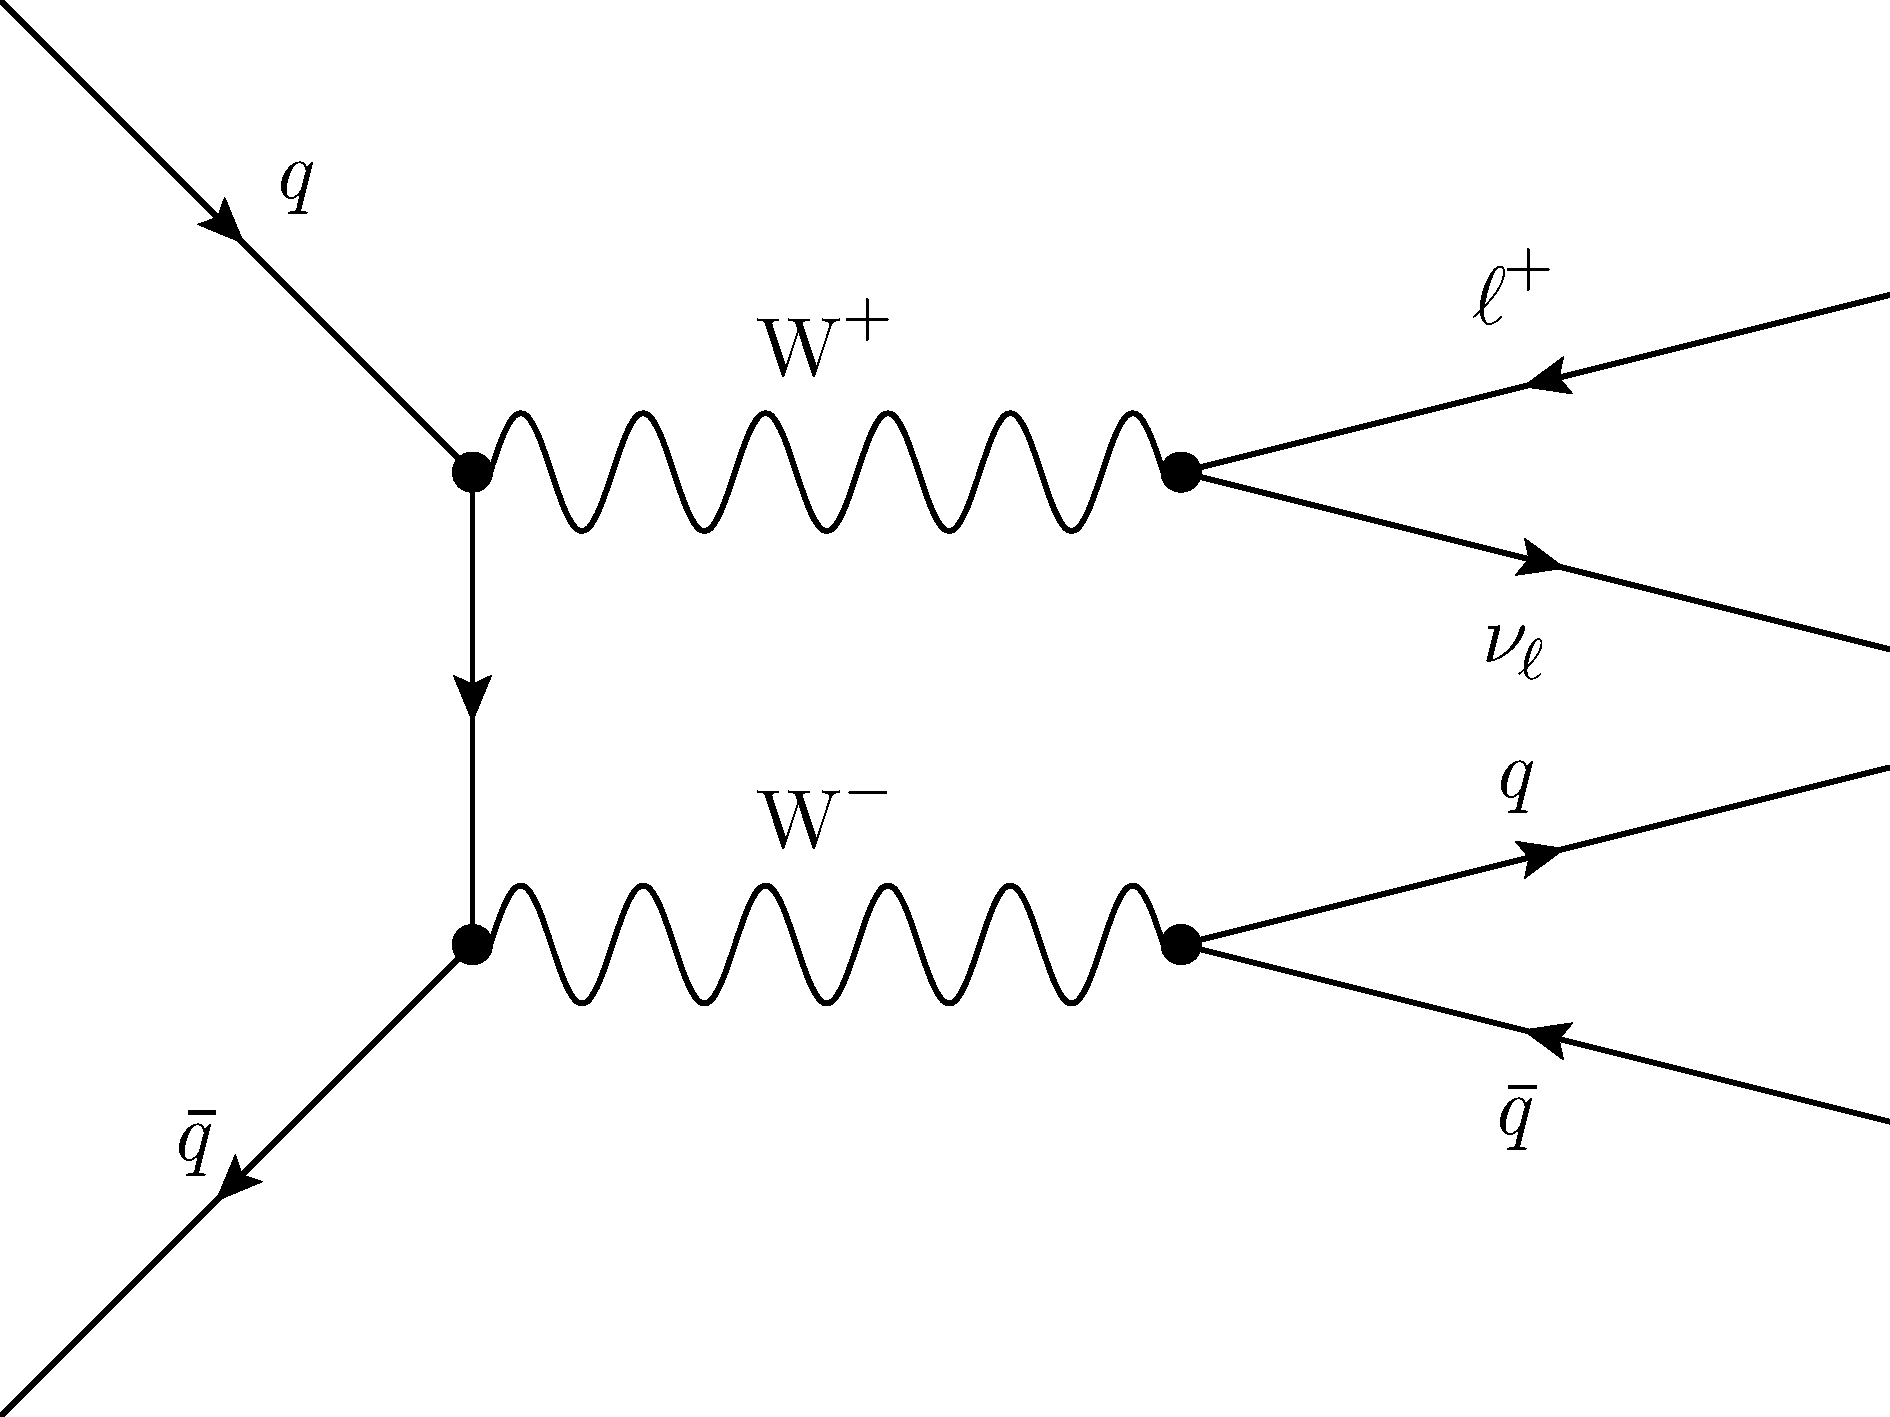
\includegraphics[width=0.48\textwidth]{\figpath/FeynmanDiagrams/WW.pdf}
				%	};
				%	\node[rectangle, rounded corners, draw=green, very thick, anchor=base] (Reducible1) at (0,2.4) {%
				%		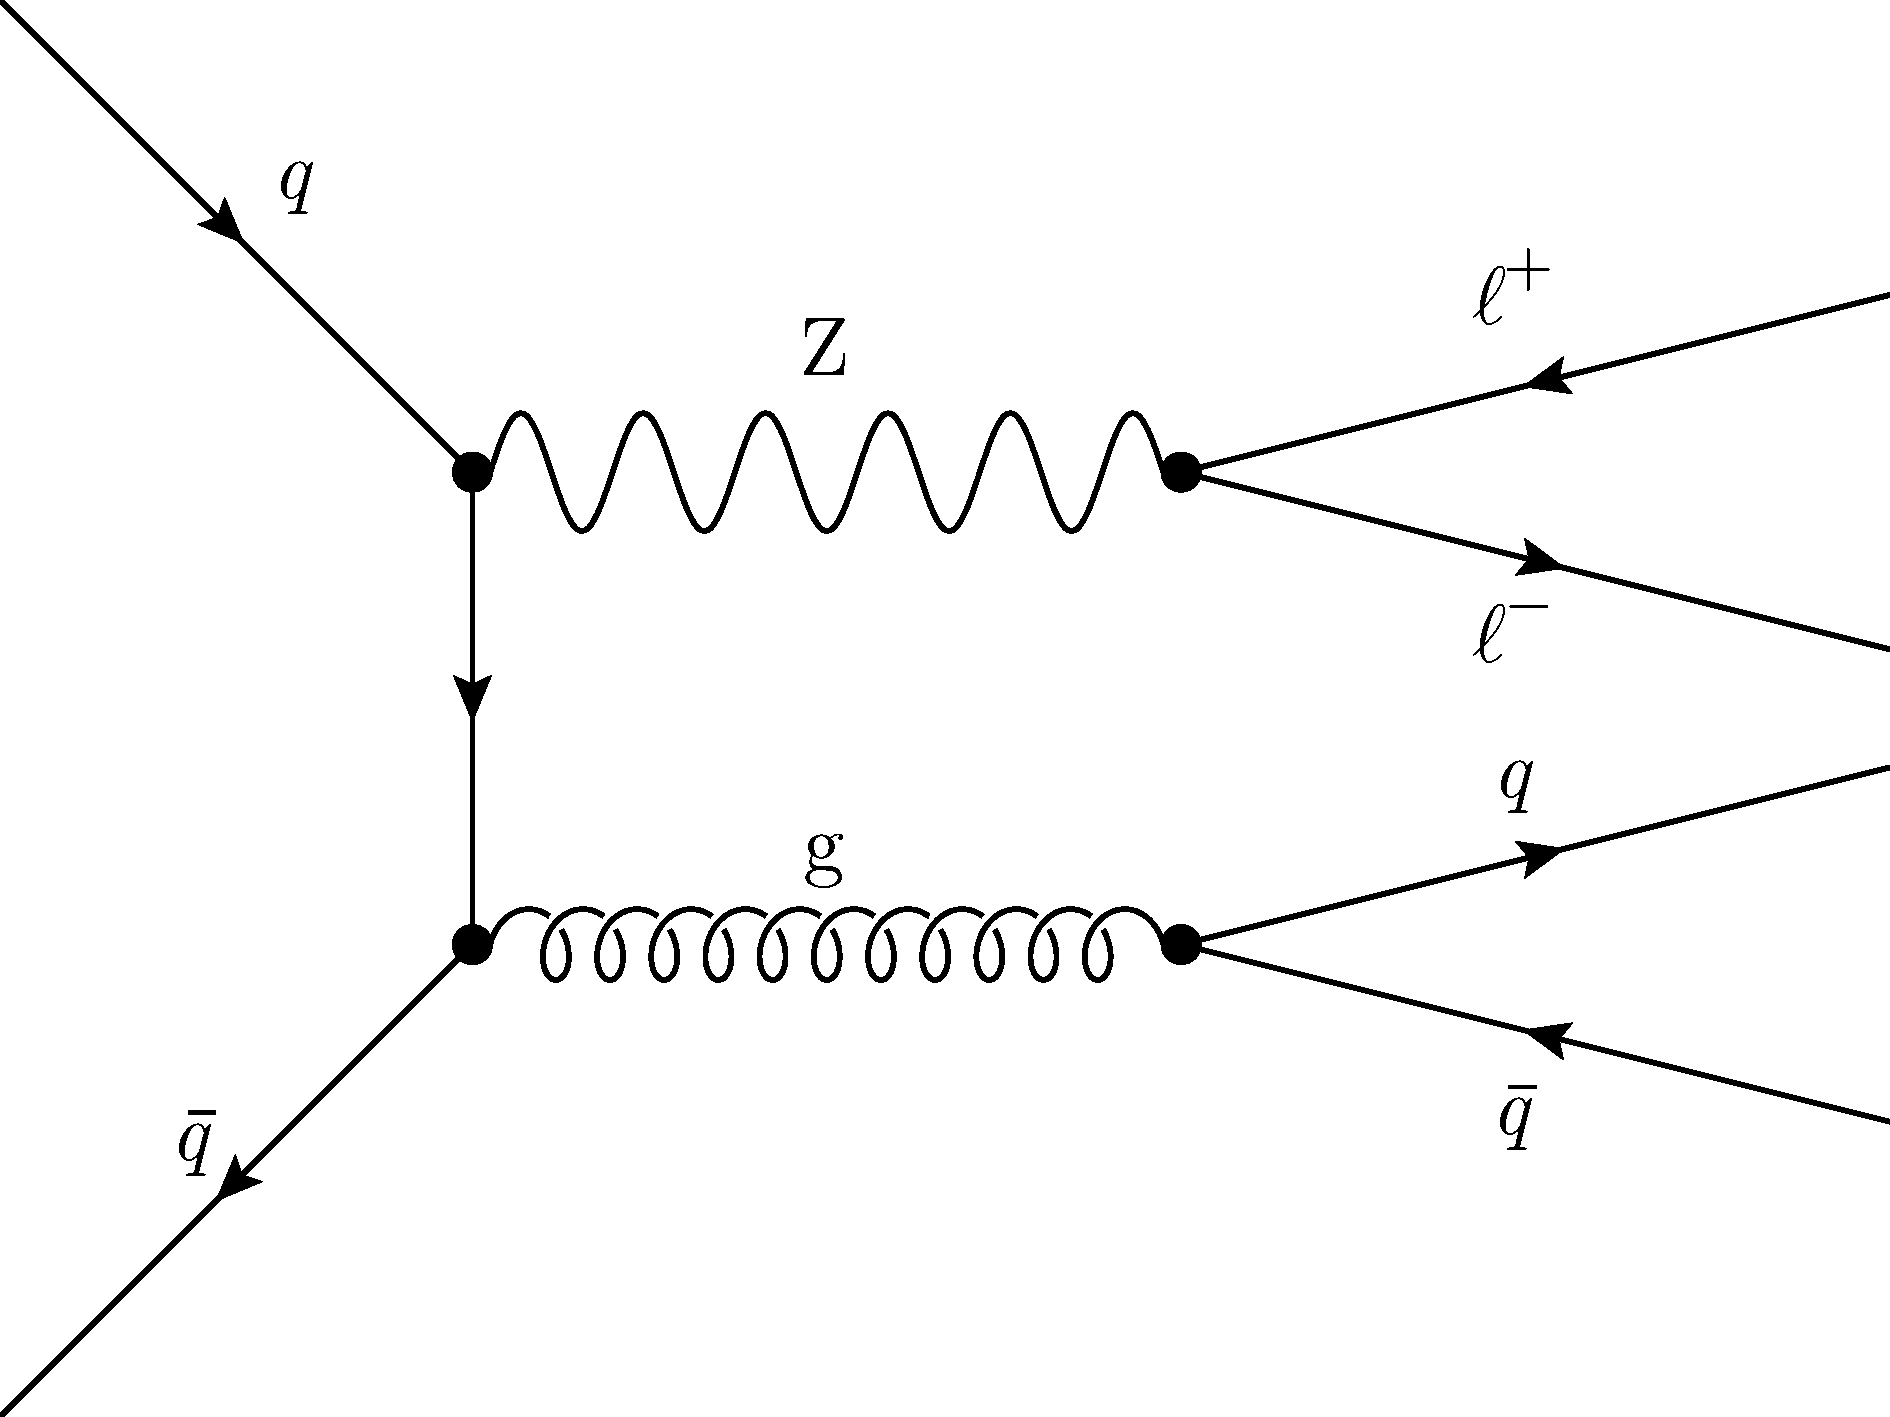
\includegraphics[width=0.31\textwidth]{\figpath/FeynmanDiagrams/ZJets.pdf}
				%		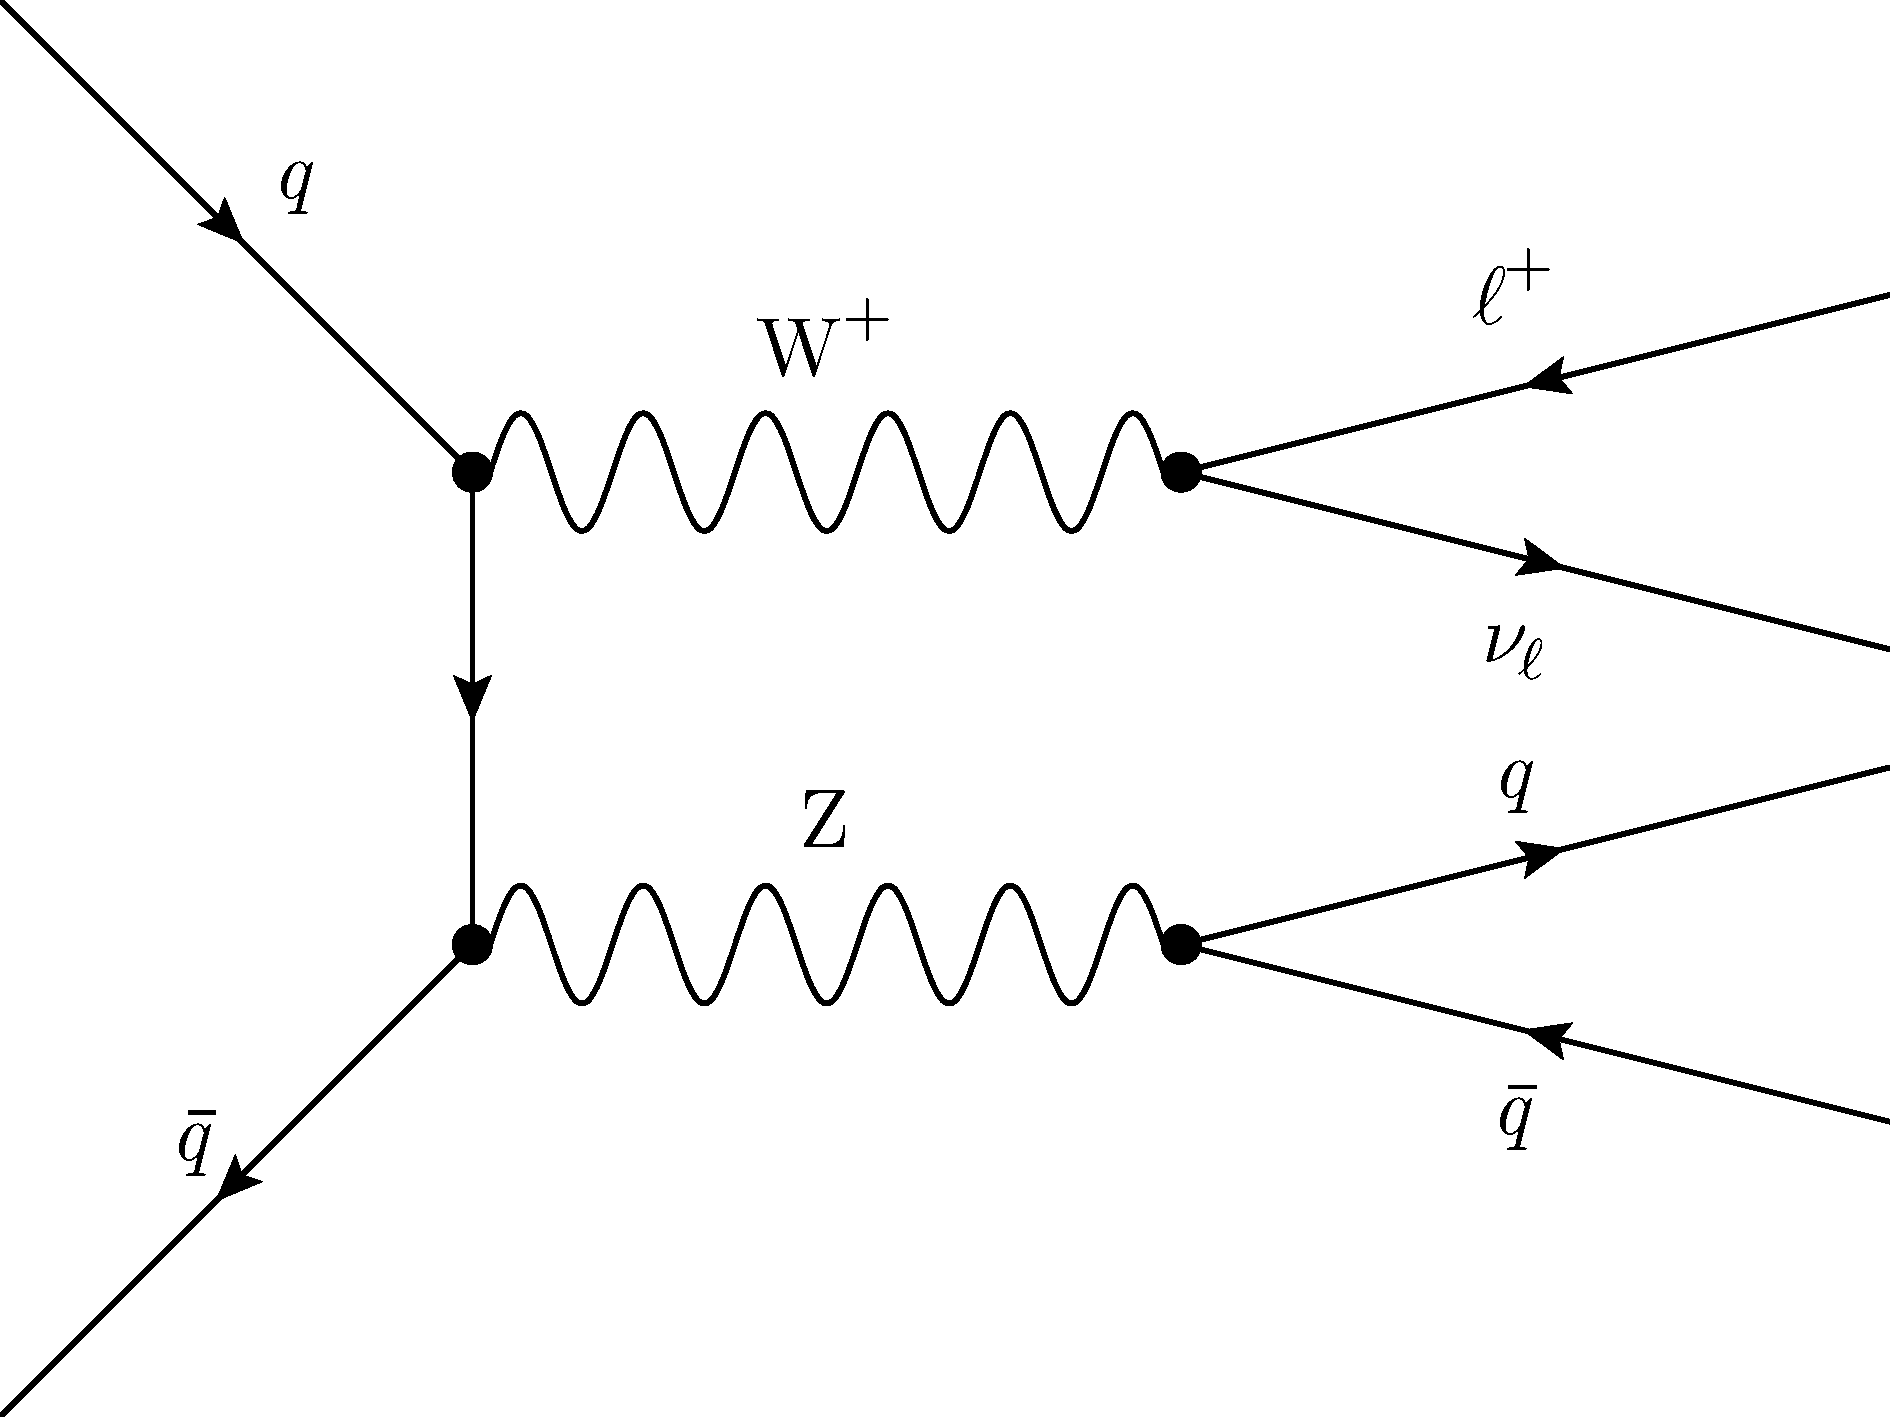
\includegraphics[width=0.31\textwidth]{\figpath/FeynmanDiagrams/WZ.pdf}
				%		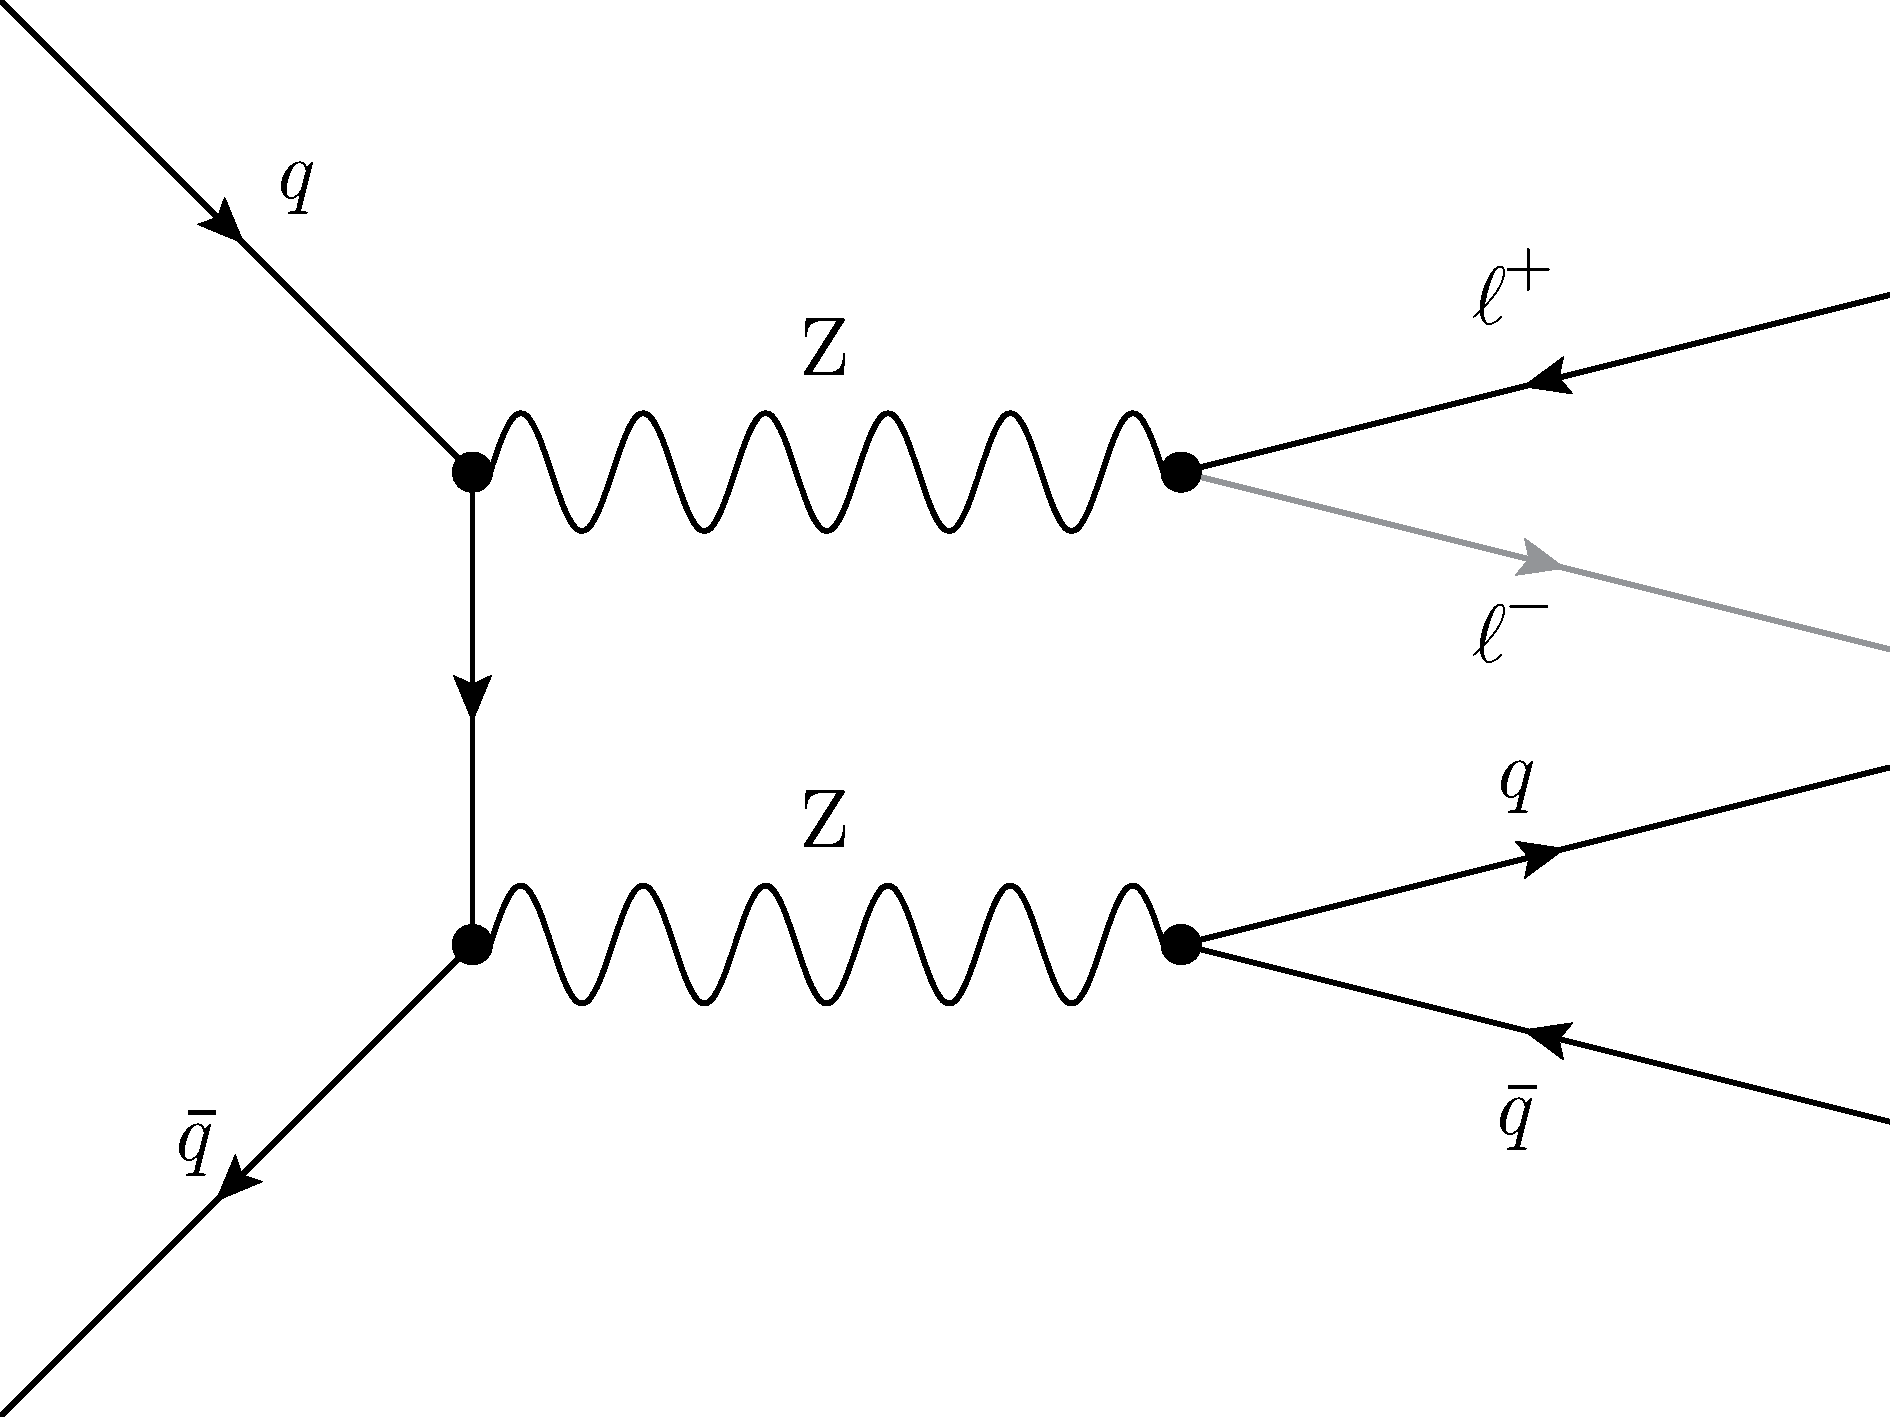
\includegraphics[width=0.31\textwidth]{\figpath/FeynmanDiagrams/ZZ.pdf}
				%	};
				%	\node[rectangle, rounded corners, draw=green, very thick, anchor=base] (Reducible2) at (0,0.5) {%
				%		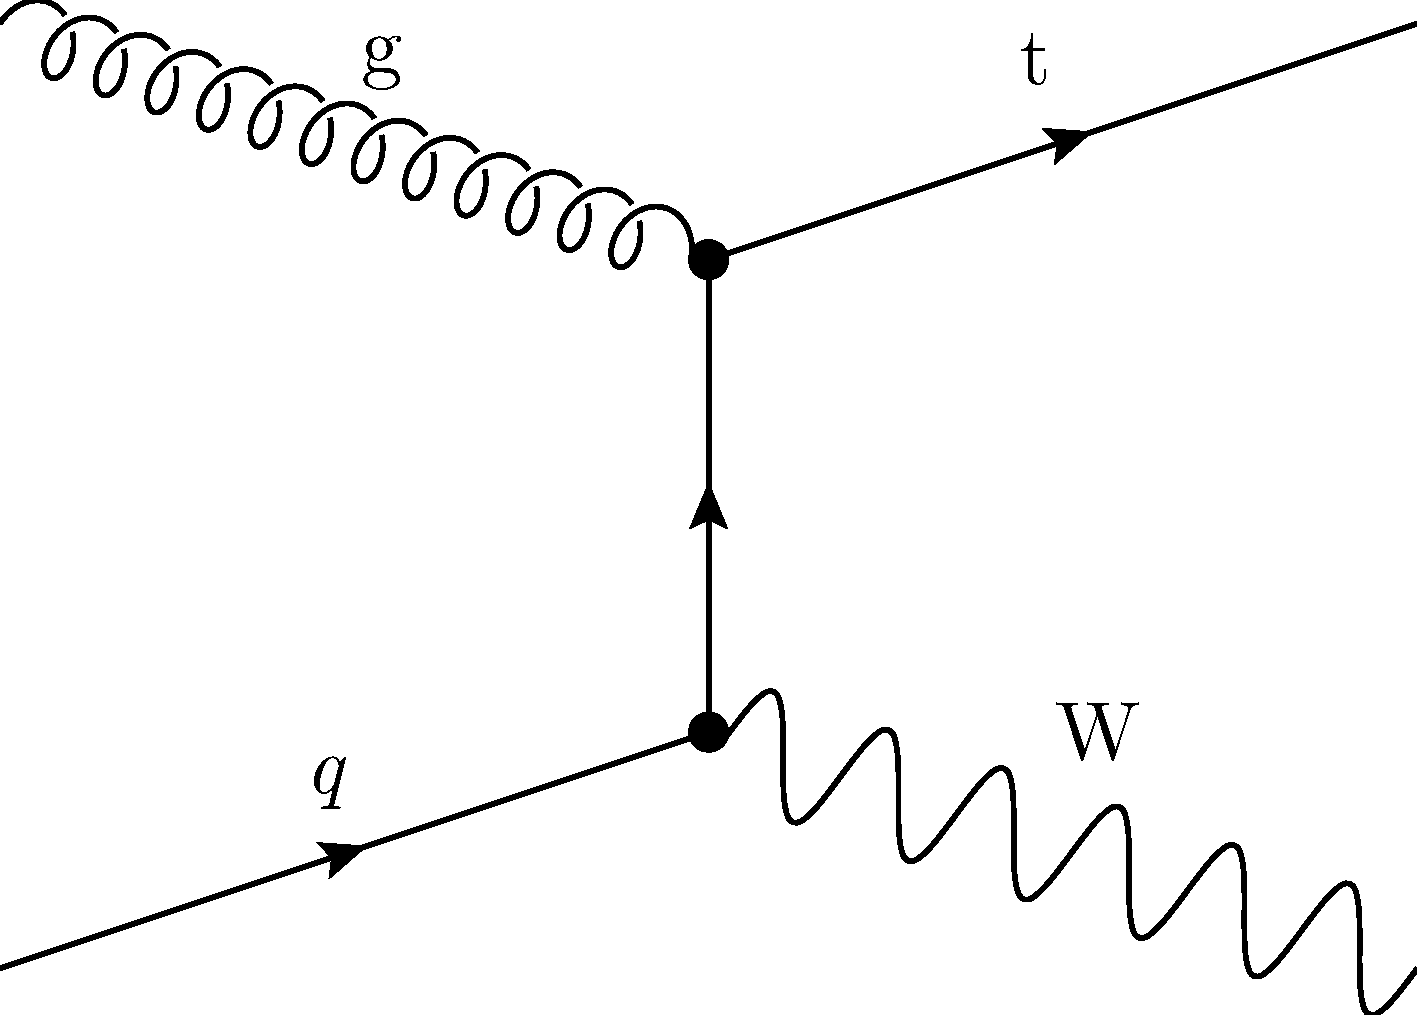
\includegraphics[width=0.31\textwidth]{\figpath/FeynmanDiagrams/STopTW.pdf}
				%		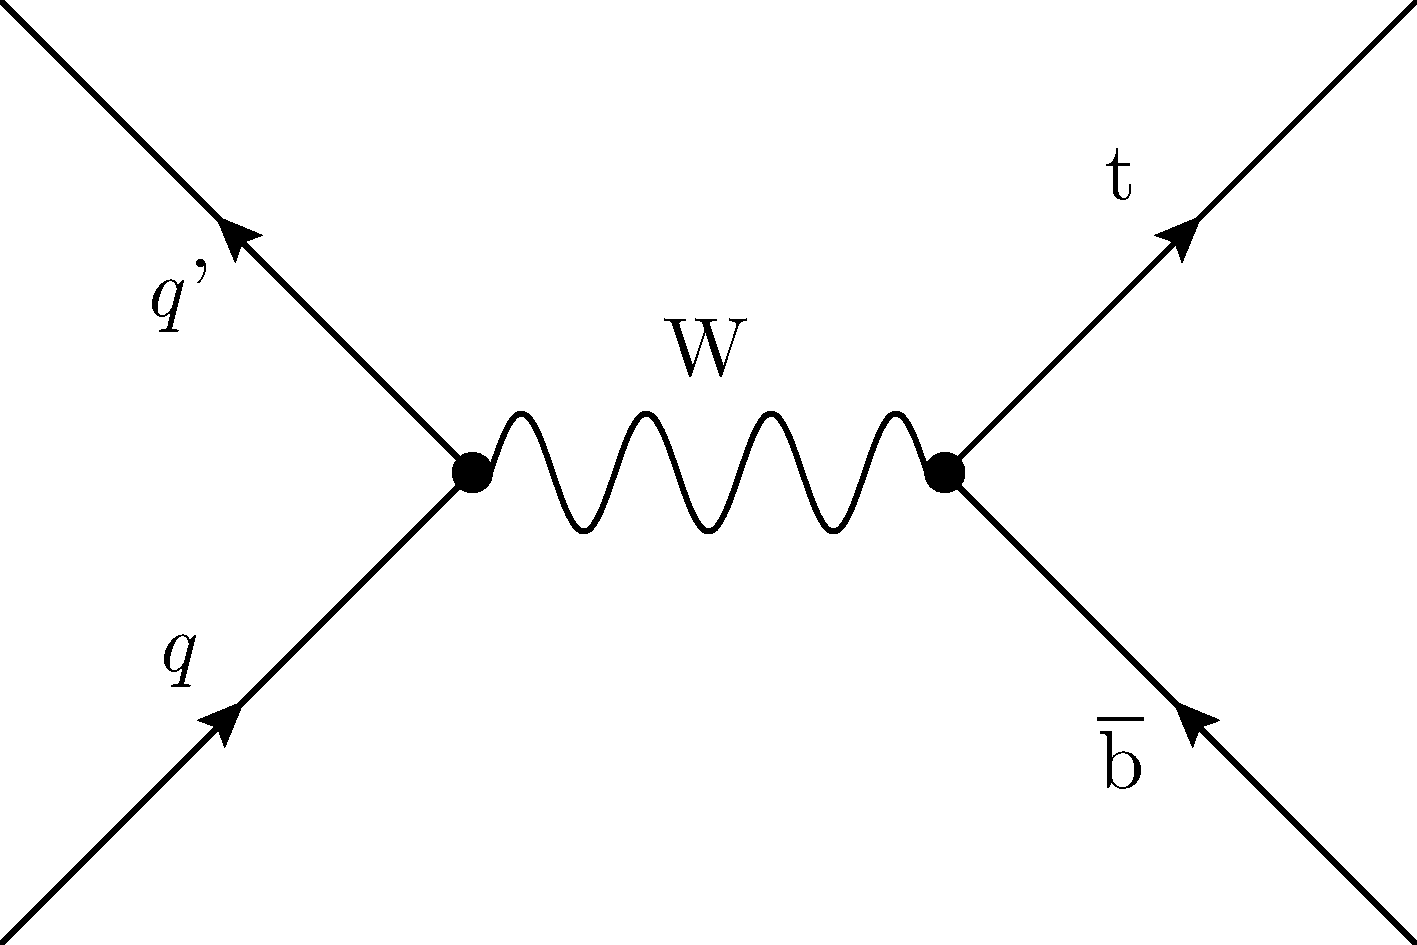
\includegraphics[width=0.31\textwidth]{\figpath/FeynmanDiagrams/STopS.pdf}
				%		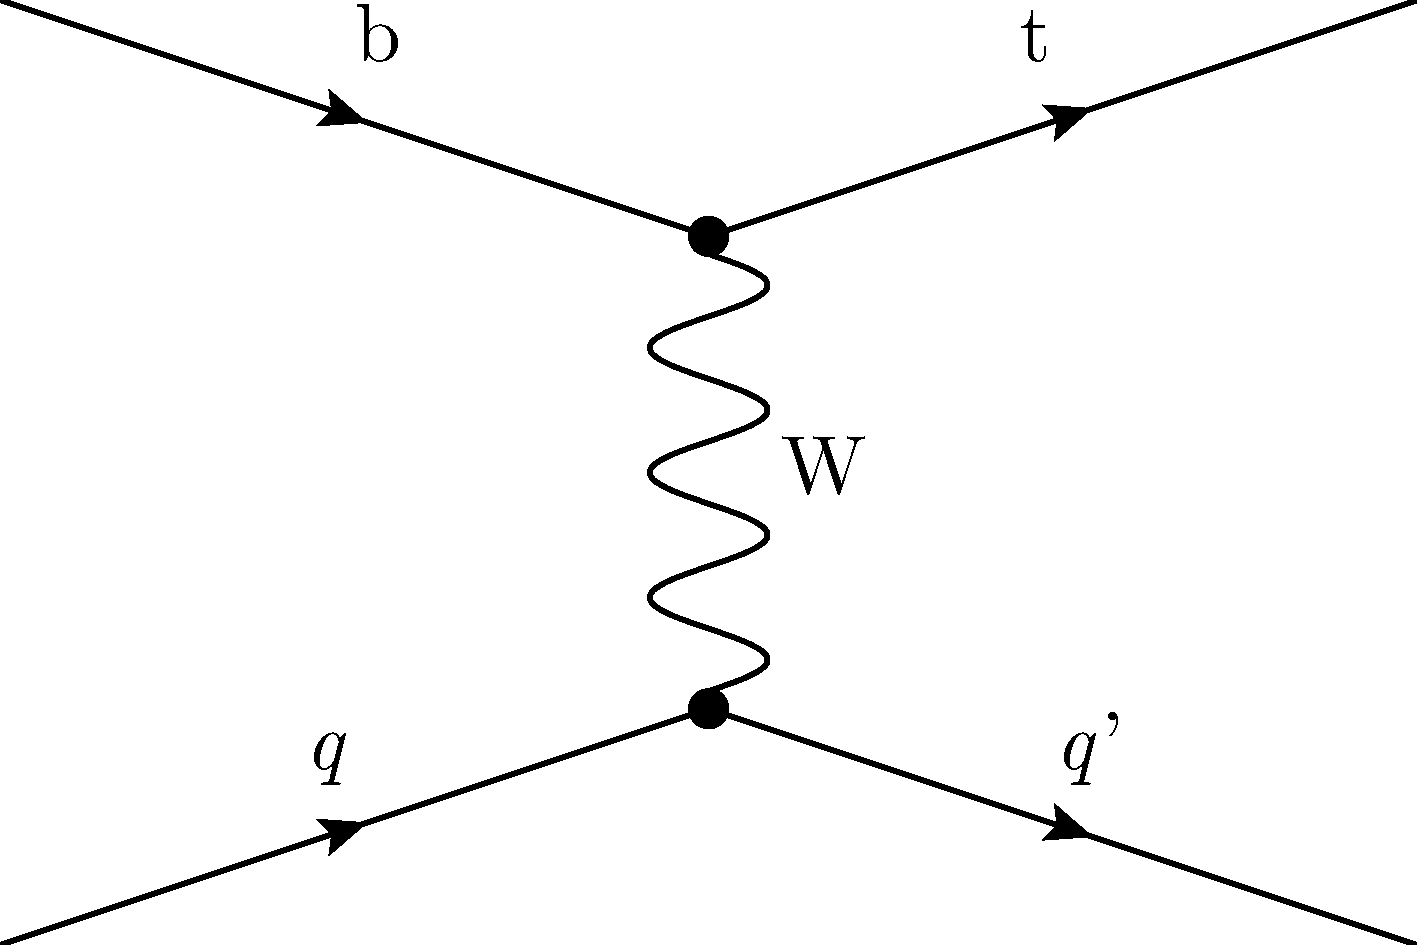
\includegraphics[width=0.31\textwidth]{\figpath/FeynmanDiagrams/STopT.pdf}
				%	};
				%	\node[rectangle, rounded corners, draw=green, very thick, anchor=base] (Reducible3) at (0,-1.5) {%
				%		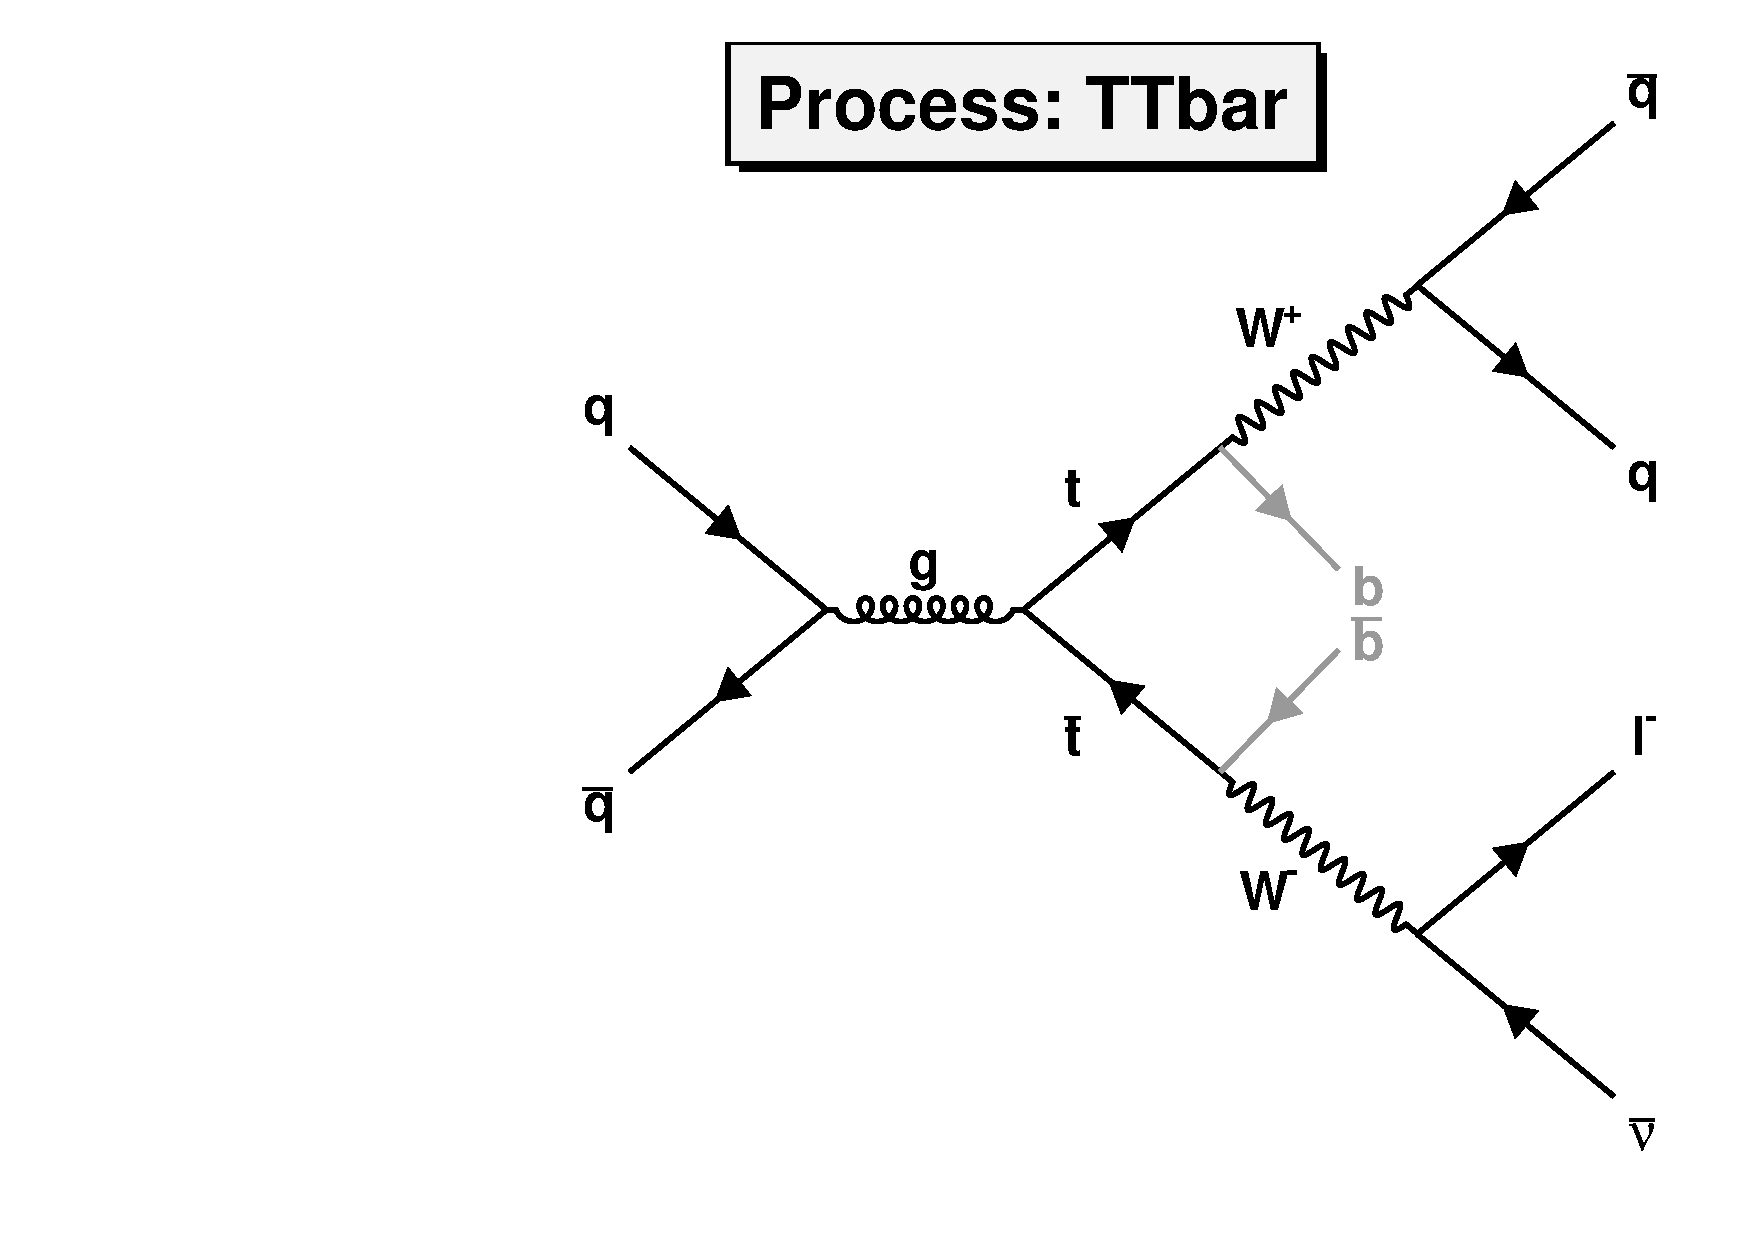
\includegraphics[width=0.31\textwidth]{\figpath/FeynmanDiagrams/TTbar.pdf}
				%		%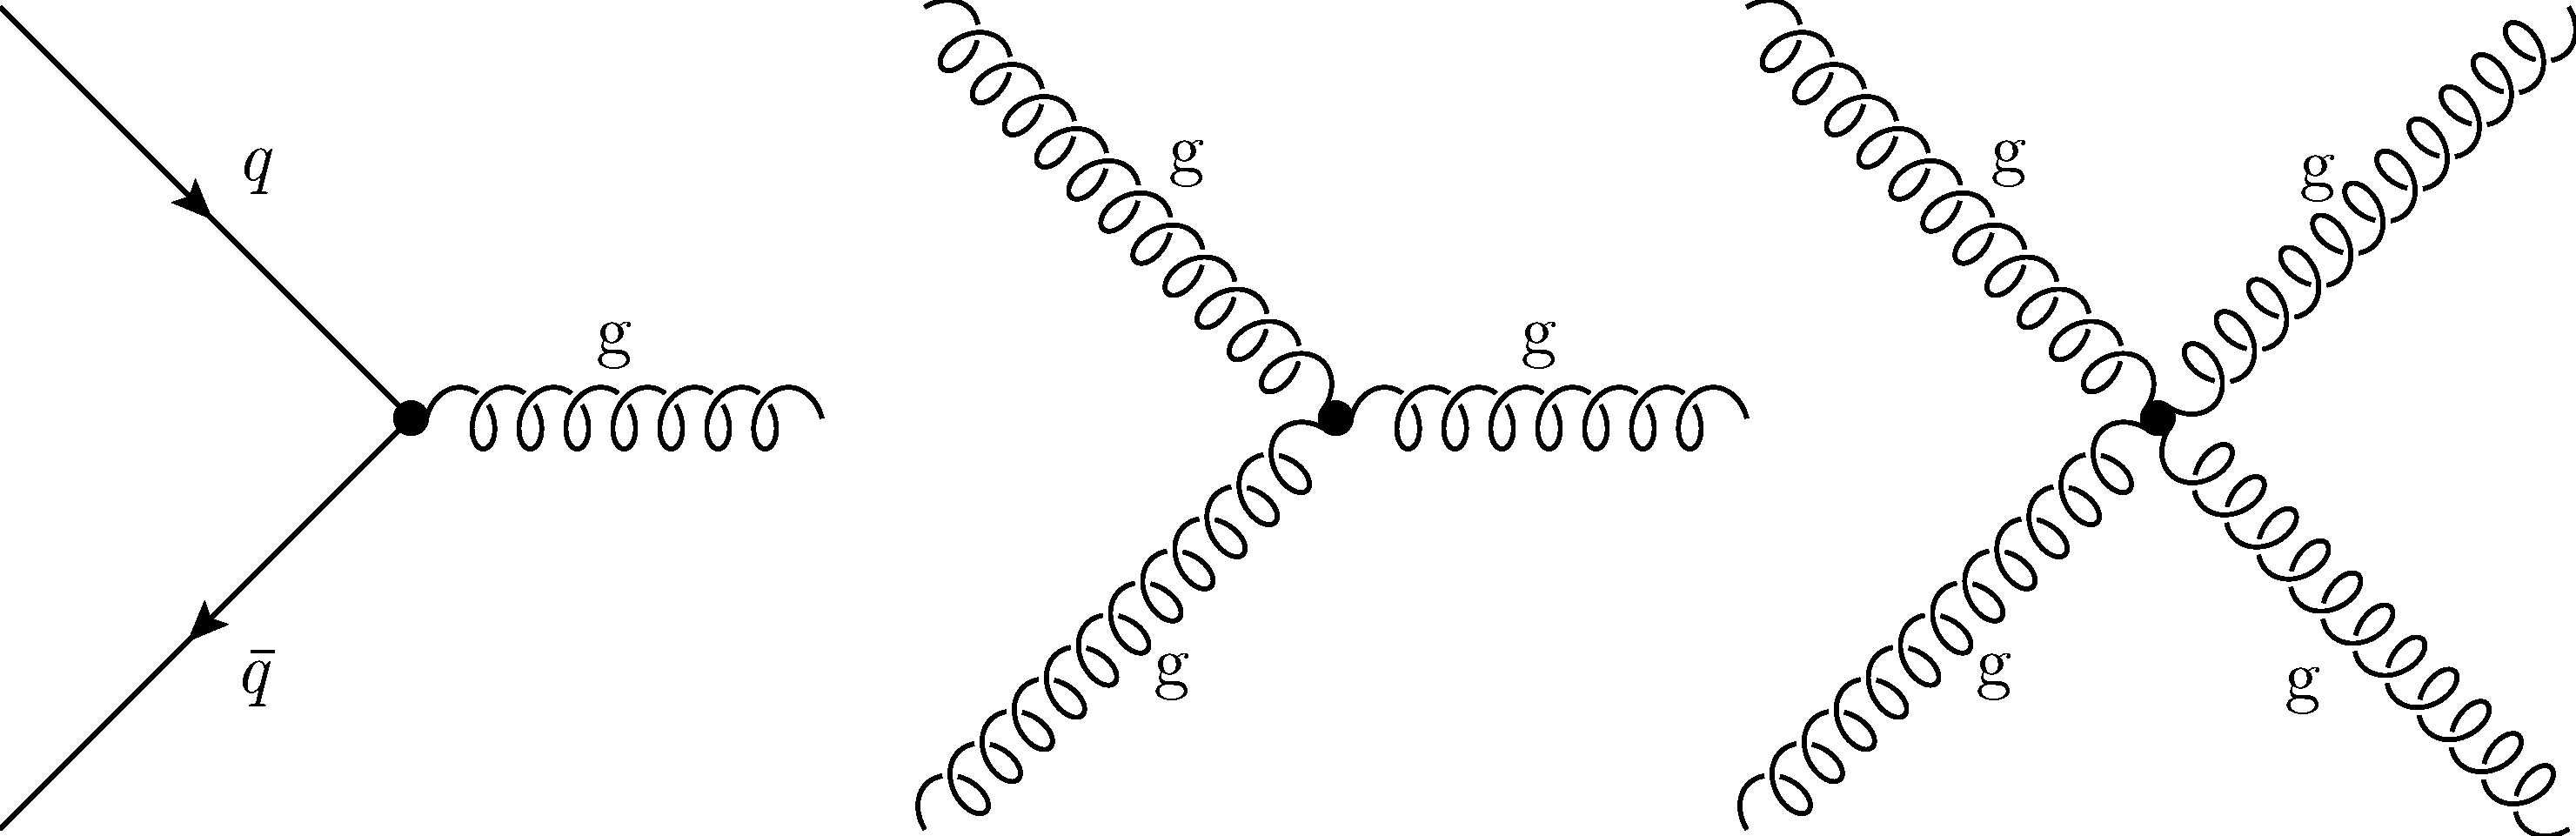
\includegraphics[width=0.48\textwidth]{\figpath/FeynmanDiagrams/QCD.pdf}
				%	};
				%}
				% define destination coordinates
				\only<2>{\node[rectangle, rounded corners, draw=red, very thick, minimum height=1em, text width=1.15em, anchor=base] (lepton) at (4.6,1.5) {};}
				\only<3>{
					\node[rectangle, rounded corners, draw=blue, very thick, minimum height=1em, text width=1.15em, anchor=base] (jet1) at (4.6,2.9) {};
					\node[rectangle, rounded corners, draw=blue, very thick, minimum height=1em, text width=1.15em, anchor=base] (jet2) at (4.6,1.8) {};
				}
				\only<4>{\node[rectangle, rounded corners, draw=ForestGreen, very thick, minimum height=1em, text width=1.15em, anchor=base] (met) at (4.6,0.4) {};}
				\only<5>{\node[rectangle, rounded corners, draw=violet, very thick, minimum height=2em, text width=1em, anchor=base] (bjet) at (3.35,2.3) {};}
			\end{tikzpicture}
		\end{column}
	\end{columns}
	% define overlays
	% Note the use of the overlay option. This is required when 
	% you want to access nodes in different pictures.
	\only<2-5>{
	\begin{tikzpicture}[overlay]
			\only<2>{\path[->,red,thick] ([xshift=1mm,yshift=1mm]s-lepton) edge [out=0,in=180] (lepton);}
			\only<3>{
				\path[->,blue,thick] ([xshift=1mm,yshift=1mm]s-jet) edge [out=0,in=180] (jet1);
				\path[->,blue,thick] ([xshift=1mm,yshift=1mm]s-jet) edge [out=0,in=180] (jet2);
			}
			\only<4>{\path[->,ForestGreen,thick] ([xshift=1mm,yshift=1mm]s-met) edge [out=0,in=180] (met);}
			\only<5>{\path[->,violet,thick] ([xshift=1mm,yshift=1mm]s-bjet) edge [out=0,in=180] (bjet);}
	\end{tikzpicture}
	}
\end{frame}
%\againframe<2>{frame:event_signature}
%\againframe<3>{frame:event_signature}
%\againframe<4>{frame:event_signature}
%\againframe<5>{frame:event_signature}
%\againframe<6>{frame:event_signature}


%%--------------------------------------------------------------------------------------------

\subsection*{SM Backgrounds}

%%--------------------------------------------------------------------------------------------

\begin{frame}
	\frametitle{SM Backgrounds}
	\vspace*{-0.24cm}
	\begin{itemize}
		\item \textit{\textbf{Irreducible}} backgrounds are those with real leptons and no b-jets
	\end{itemize}
	\vspace*{-0.2cm}
	\begin{table}[tb]
		\centering
		\begin{tabular}{>{\centering}m{0.15\textwidth} >{\centering}m{0.27\textwidth} | >{\centering}m{0.15\textwidth} >{\centering\arraybackslash}m{0.27\textwidth}}
			\Wjets & 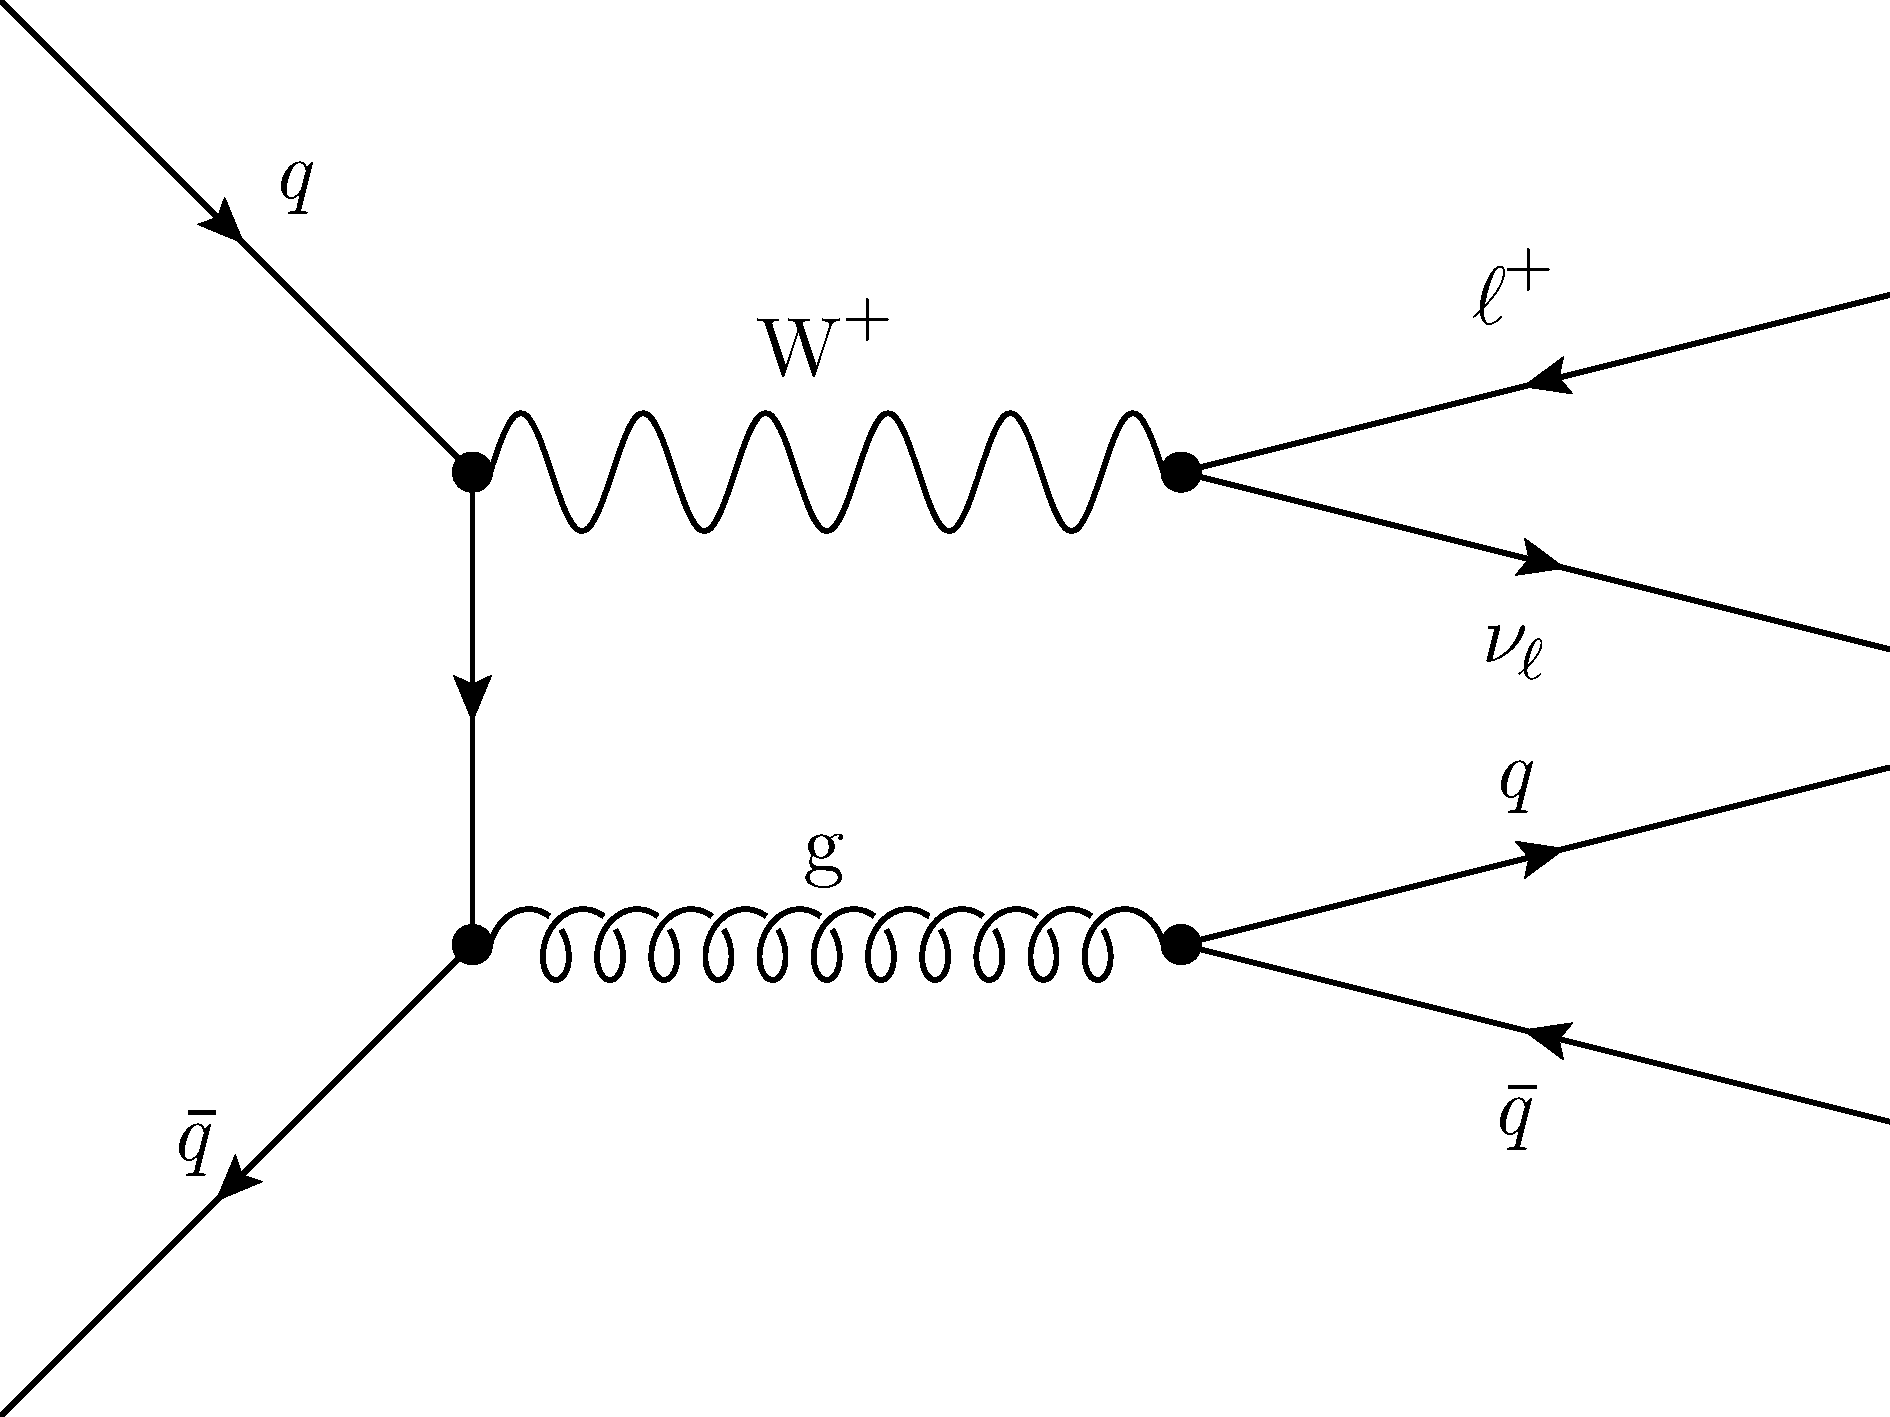
\includegraphics[width=0.25\textwidth]{\figpath/FeynmanDiagrams/WJets.pdf} & \WW & 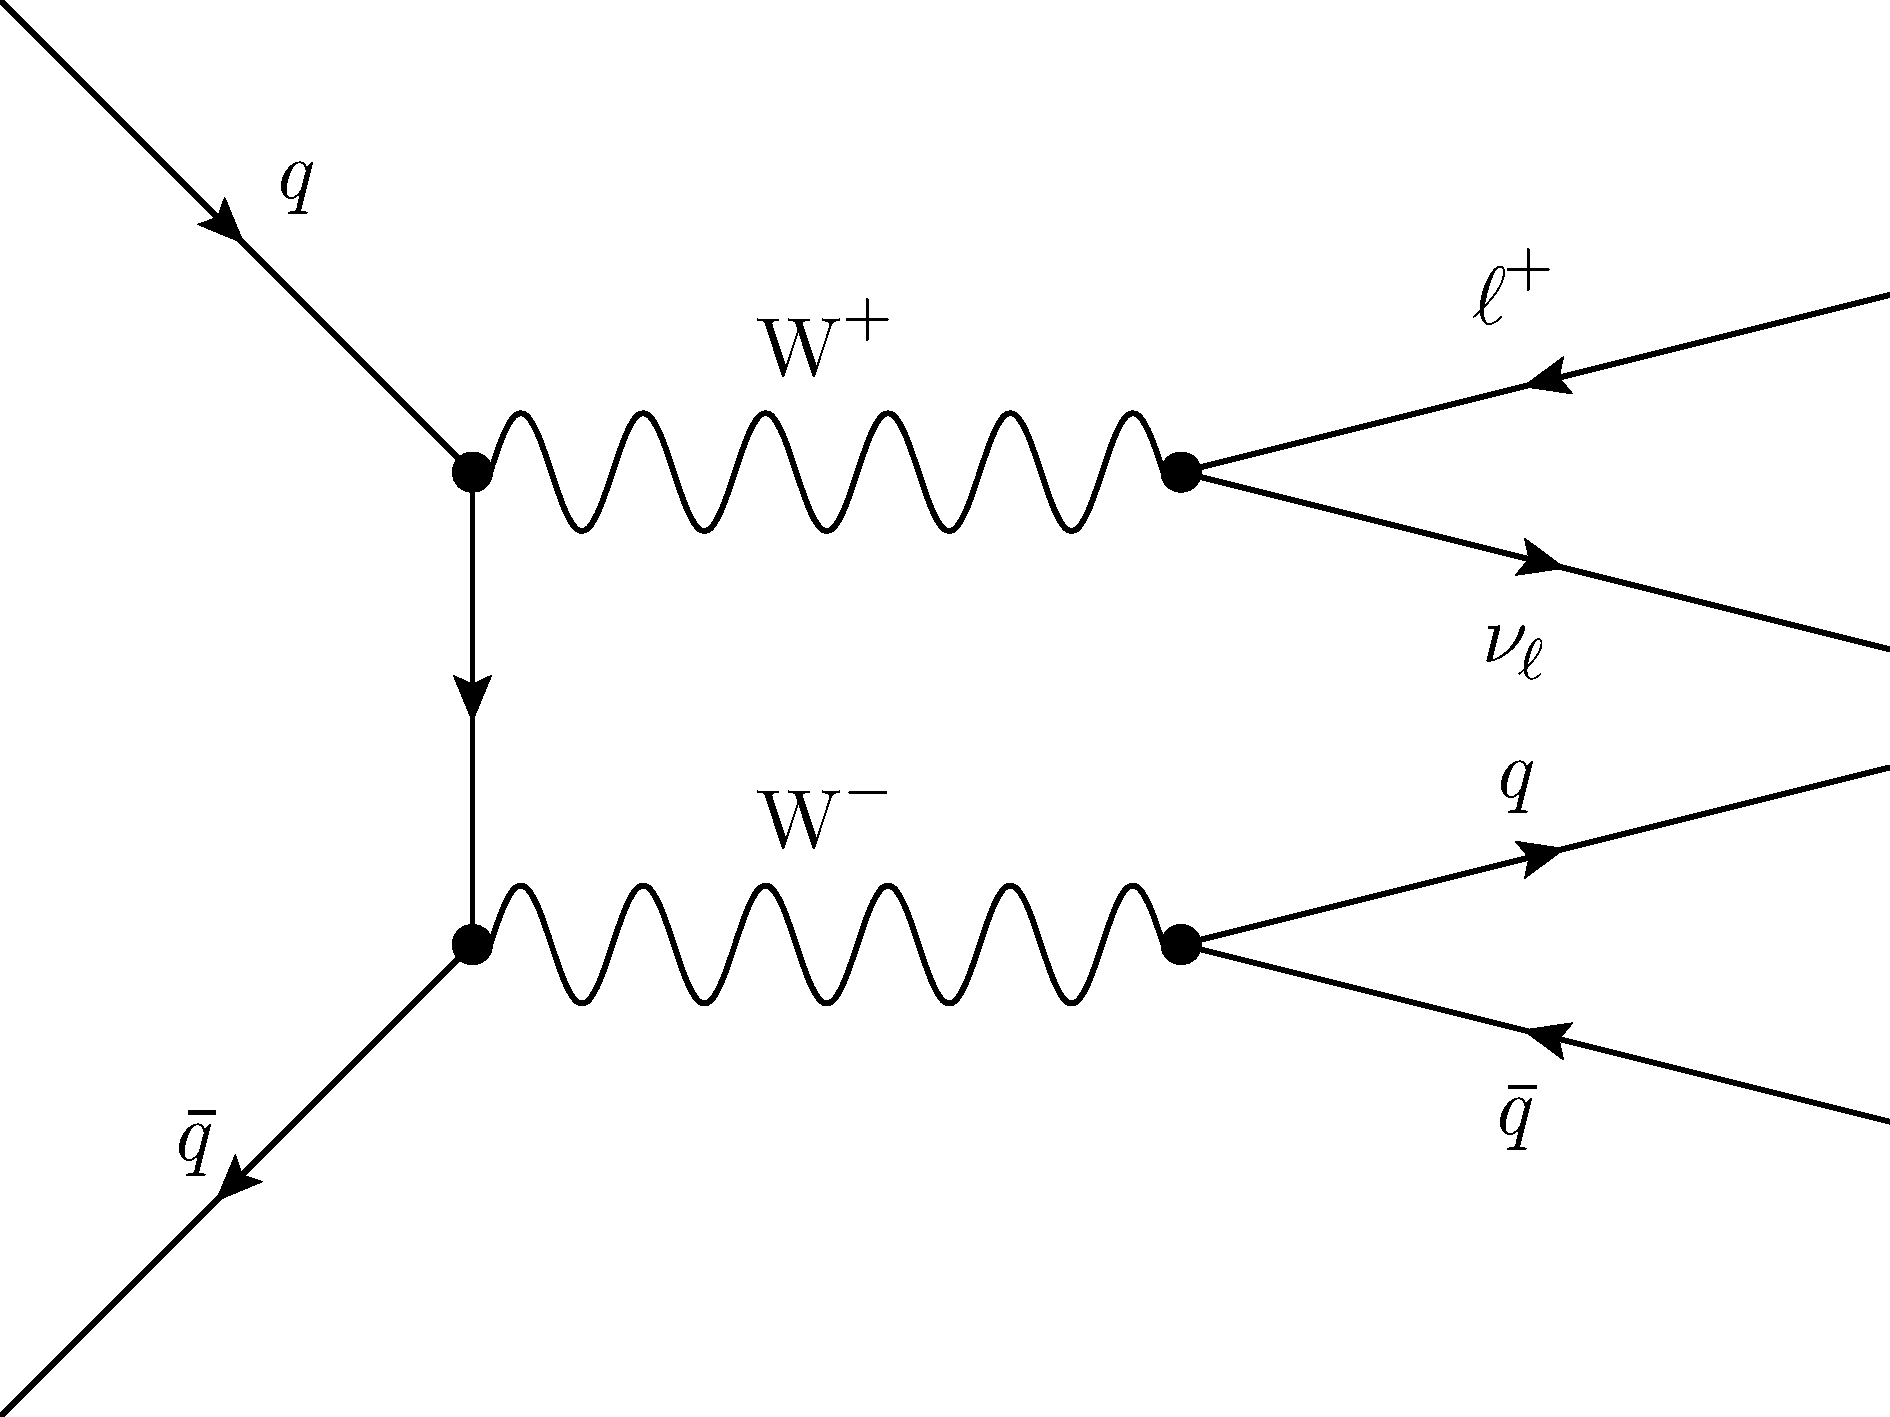
\includegraphics[width=0.25\textwidth]{\figpath/FeynmanDiagrams/WW.pdf} \\
			\WZ & 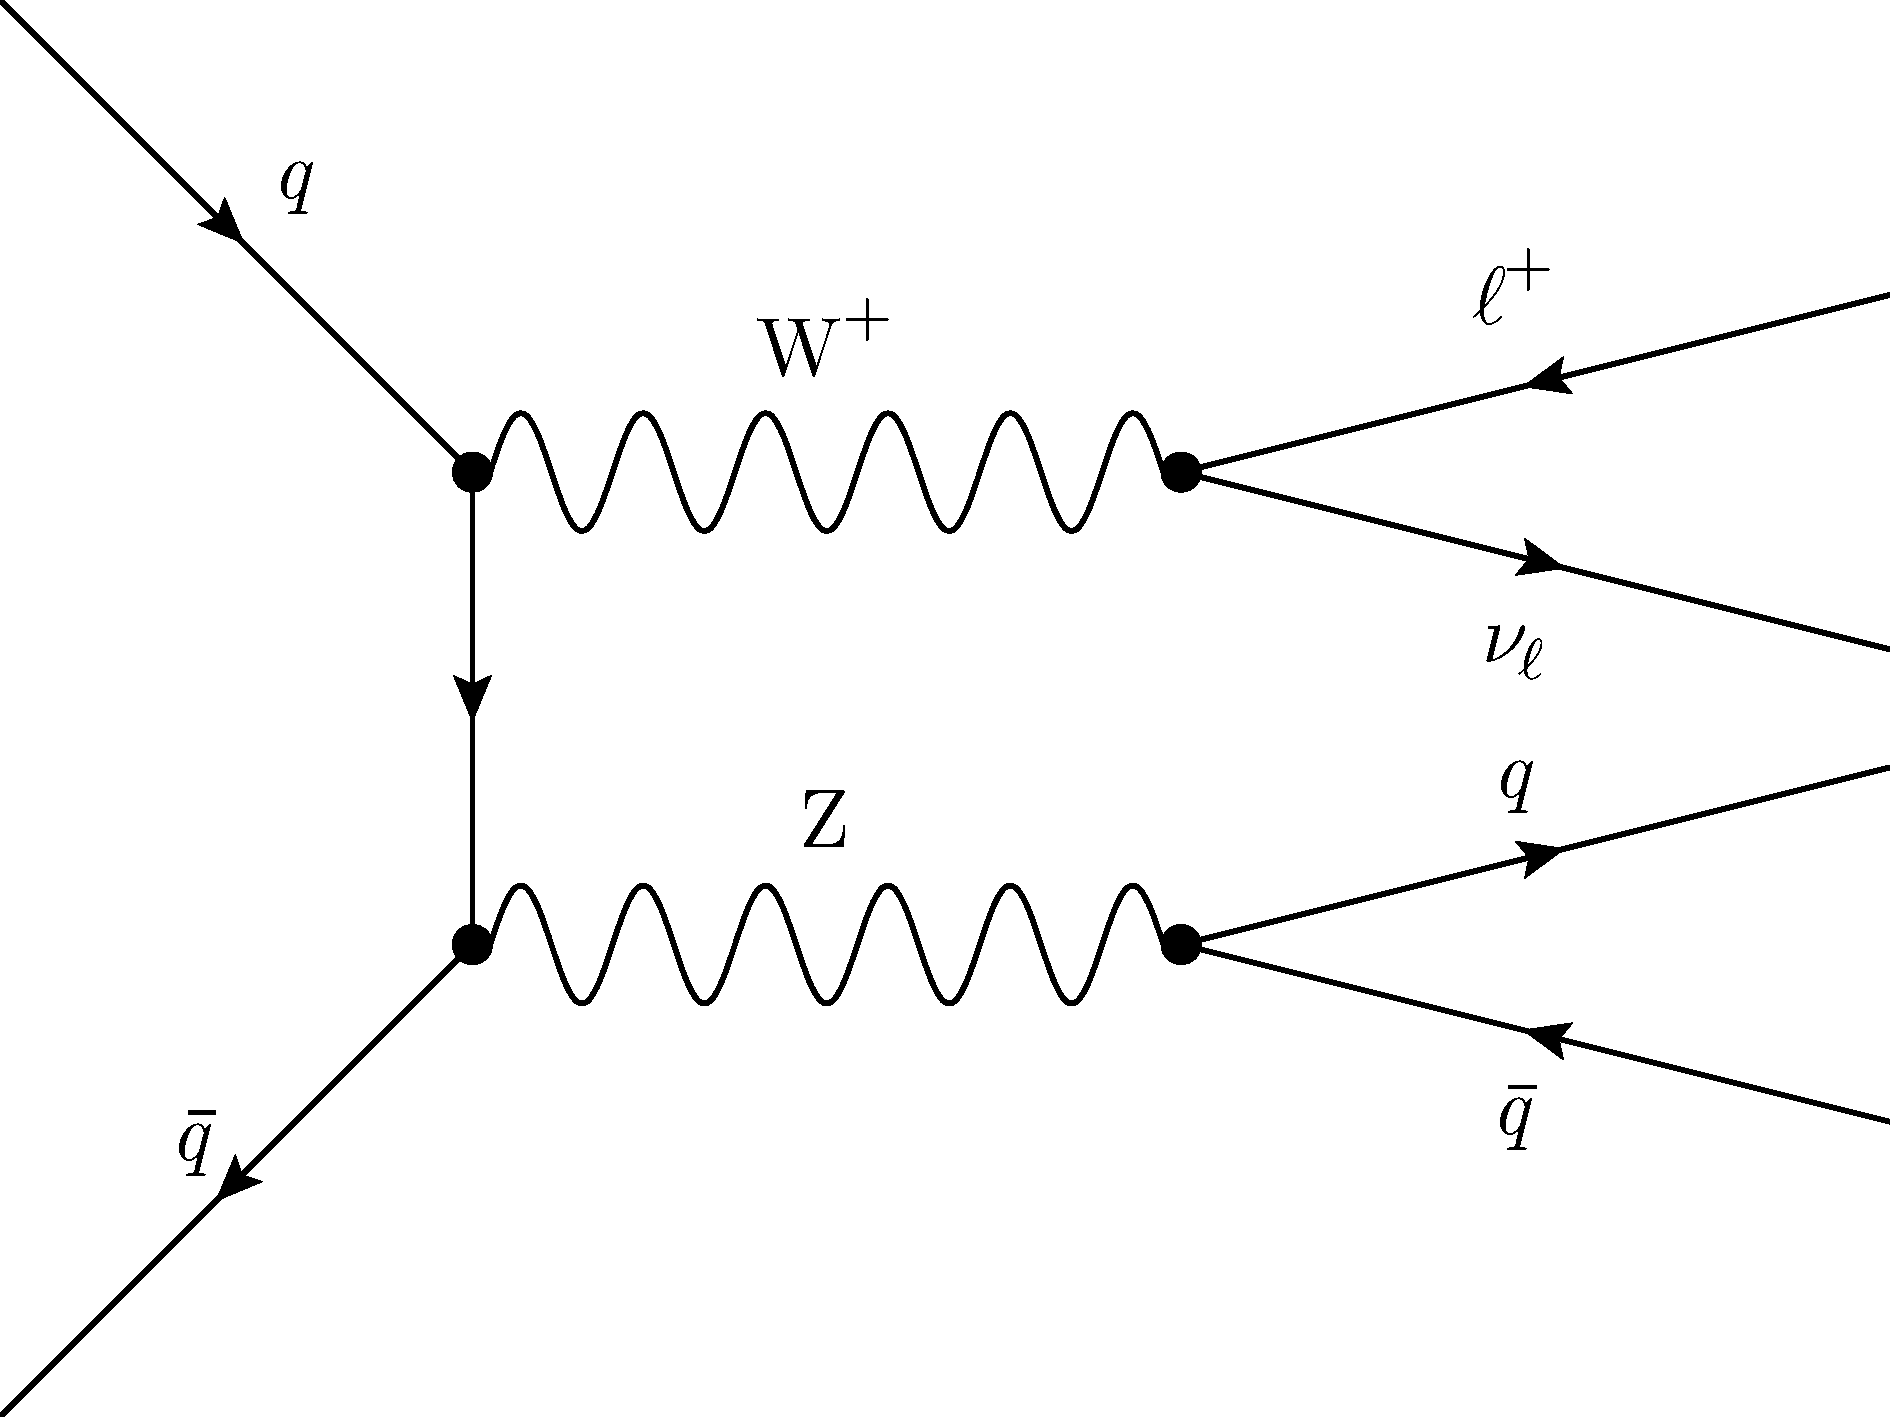
\includegraphics[width=0.25\textwidth]{\figpath/FeynmanDiagrams/WZ.pdf} & & \\
		\end{tabular}
	\end{table}
	\vspace*{-0.2cm}
	\begin{itemize}
		\item \textit{\textbf{Reducible}} backgrounds are those with fake (extra) leptons or b-jets
	\end{itemize}
	\vspace*{-0.2cm}
	\begin{table}[tb]
		\centering
		\begin{tabular}{>{\centering}m{0.15\textwidth} >{\centering}m{0.27\textwidth} | >{\centering}m{0.15\textwidth} >{\centering\arraybackslash}m{0.27\textwidth}}
			  \ttbar & 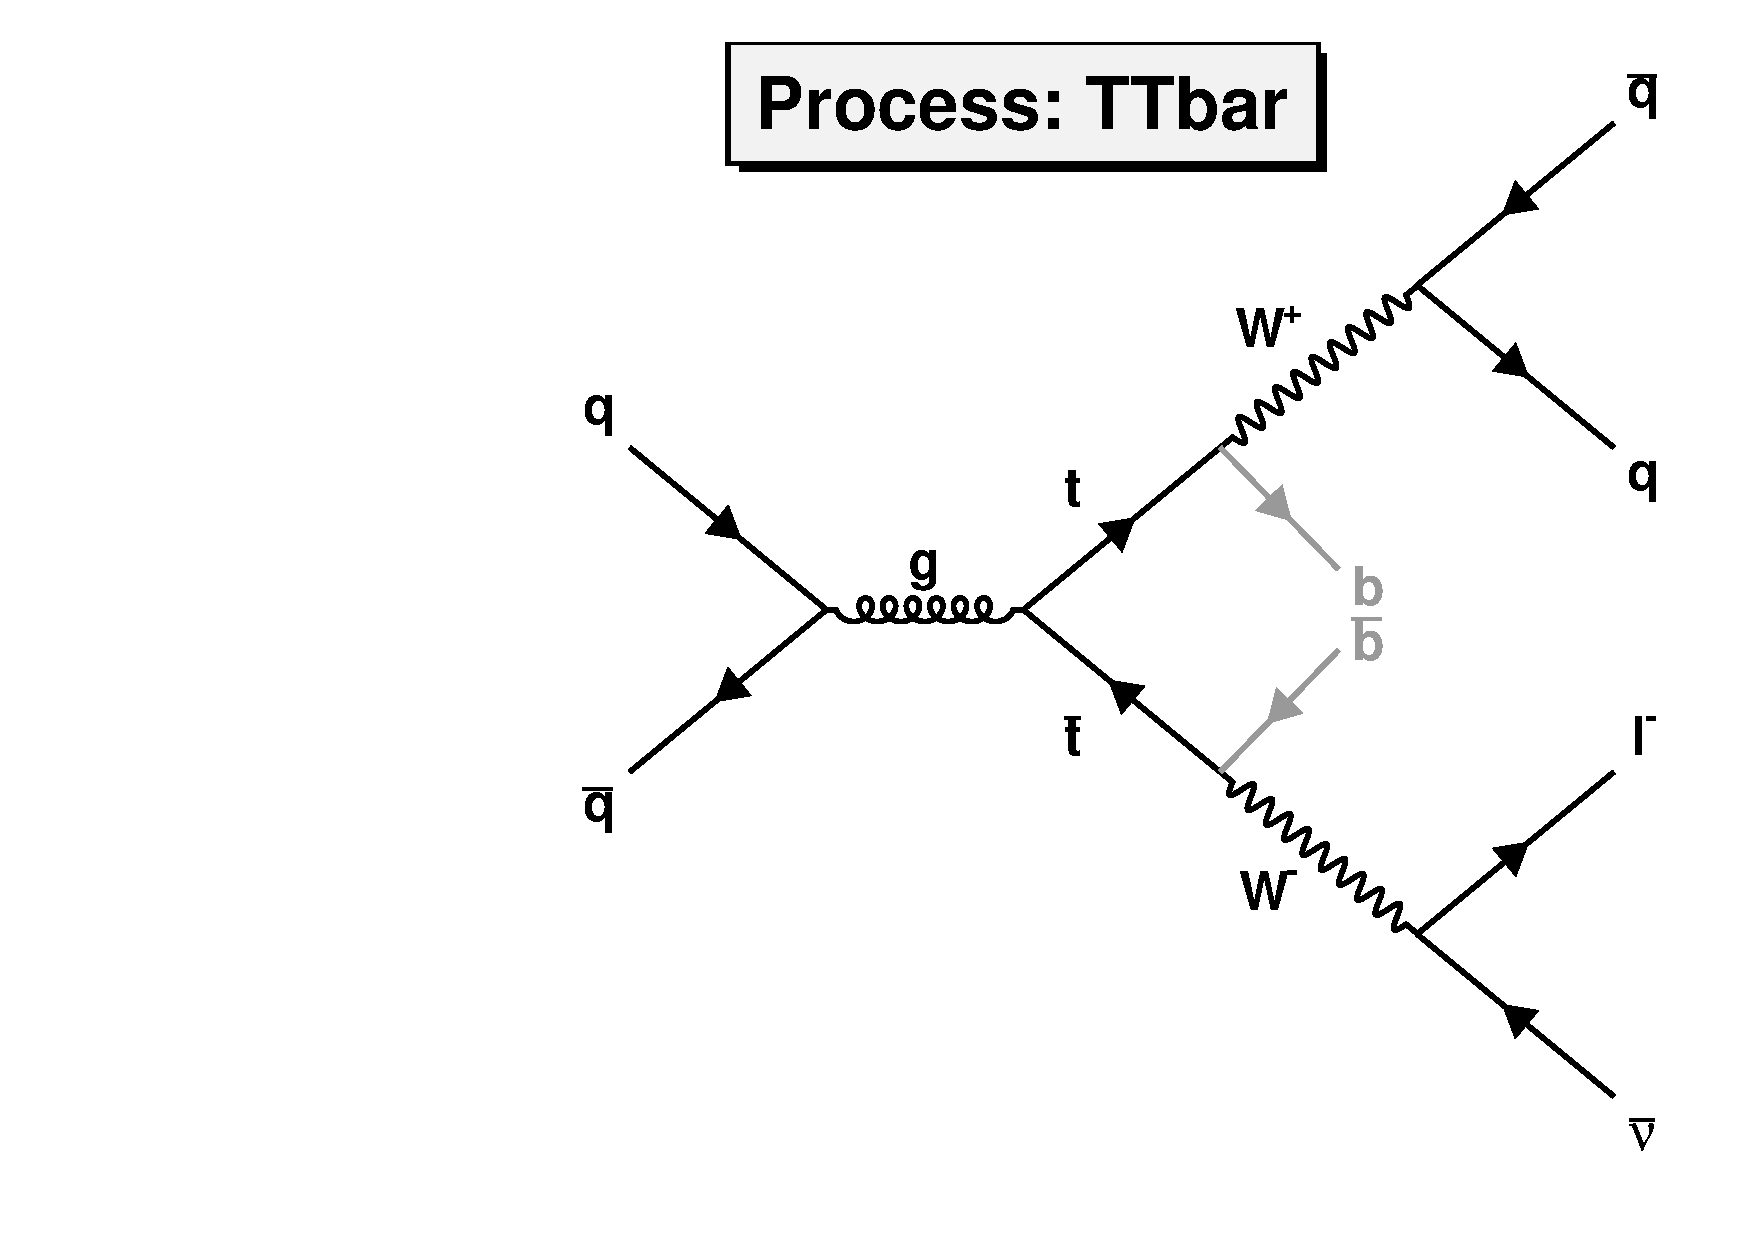
\includegraphics[width=0.25\textwidth]{\figpath/FeynmanDiagrams/TTbar.pdf} & & \\
		\end{tabular}
	\end{table}
\end{frame}

\begin{frame}
	\frametitle{SM Backgrounds}
	\vspace*{-0.24cm}
	\begin{itemize}
		\item \textit{\textbf{Reducible}} backgrounds continued \ldots
	\end{itemize}
	\begin{table}[tb]
		\centering
		\begin{tabular}{>{\centering}m{0.15\textwidth} >{\centering}m{0.27\textwidth} | >{\centering}m{0.15\textwidth} >{\centering\arraybackslash}m{0.27\textwidth}}
			\Zjets & 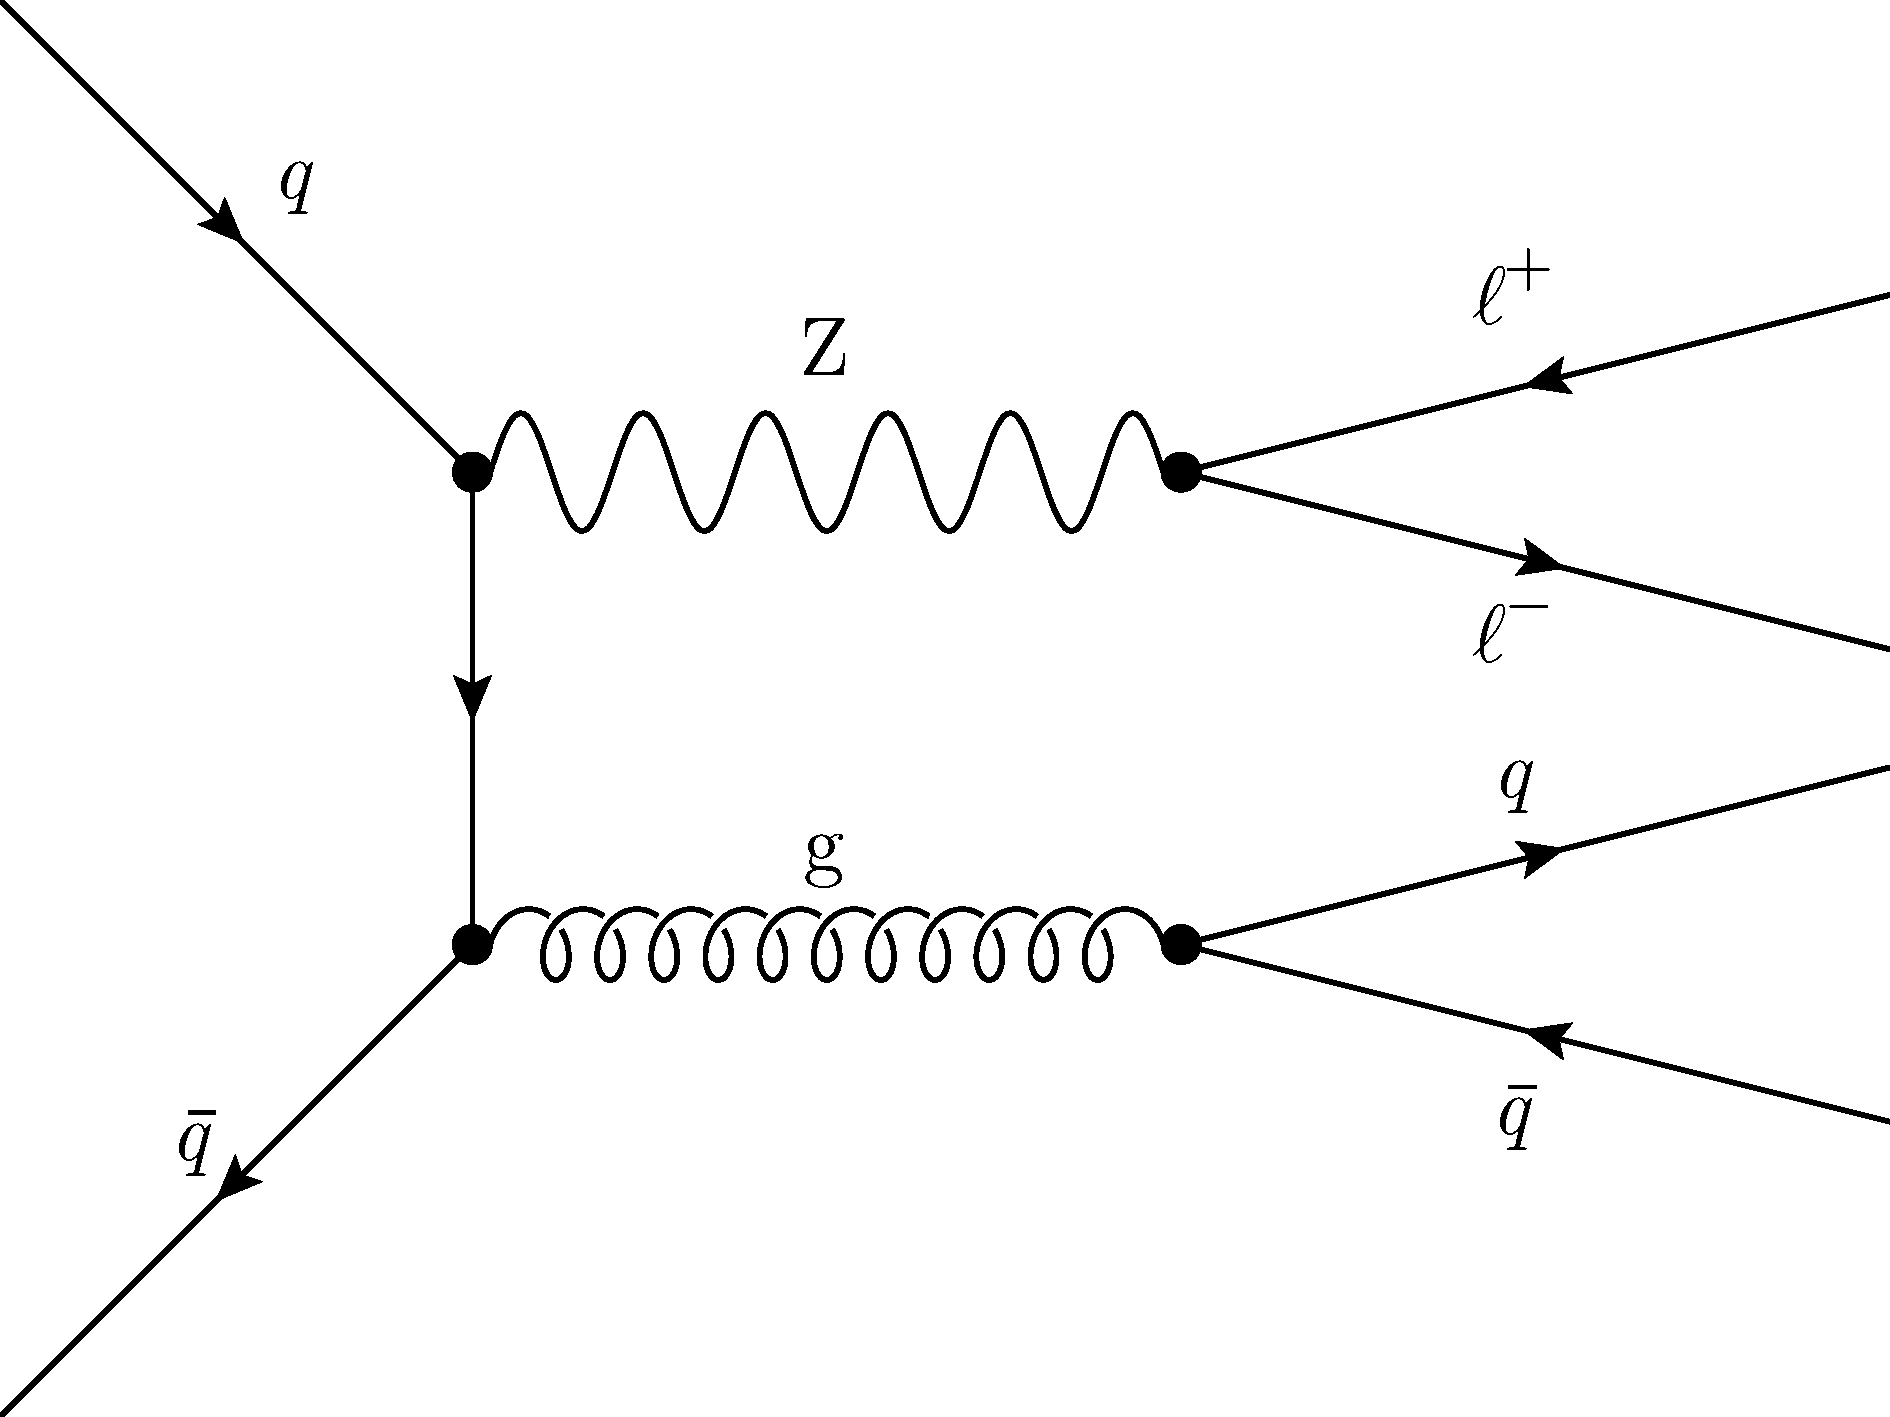
\includegraphics[width=0.25\textwidth]{\figpath/FeynmanDiagrams/ZJets.pdf} & \ZZ & 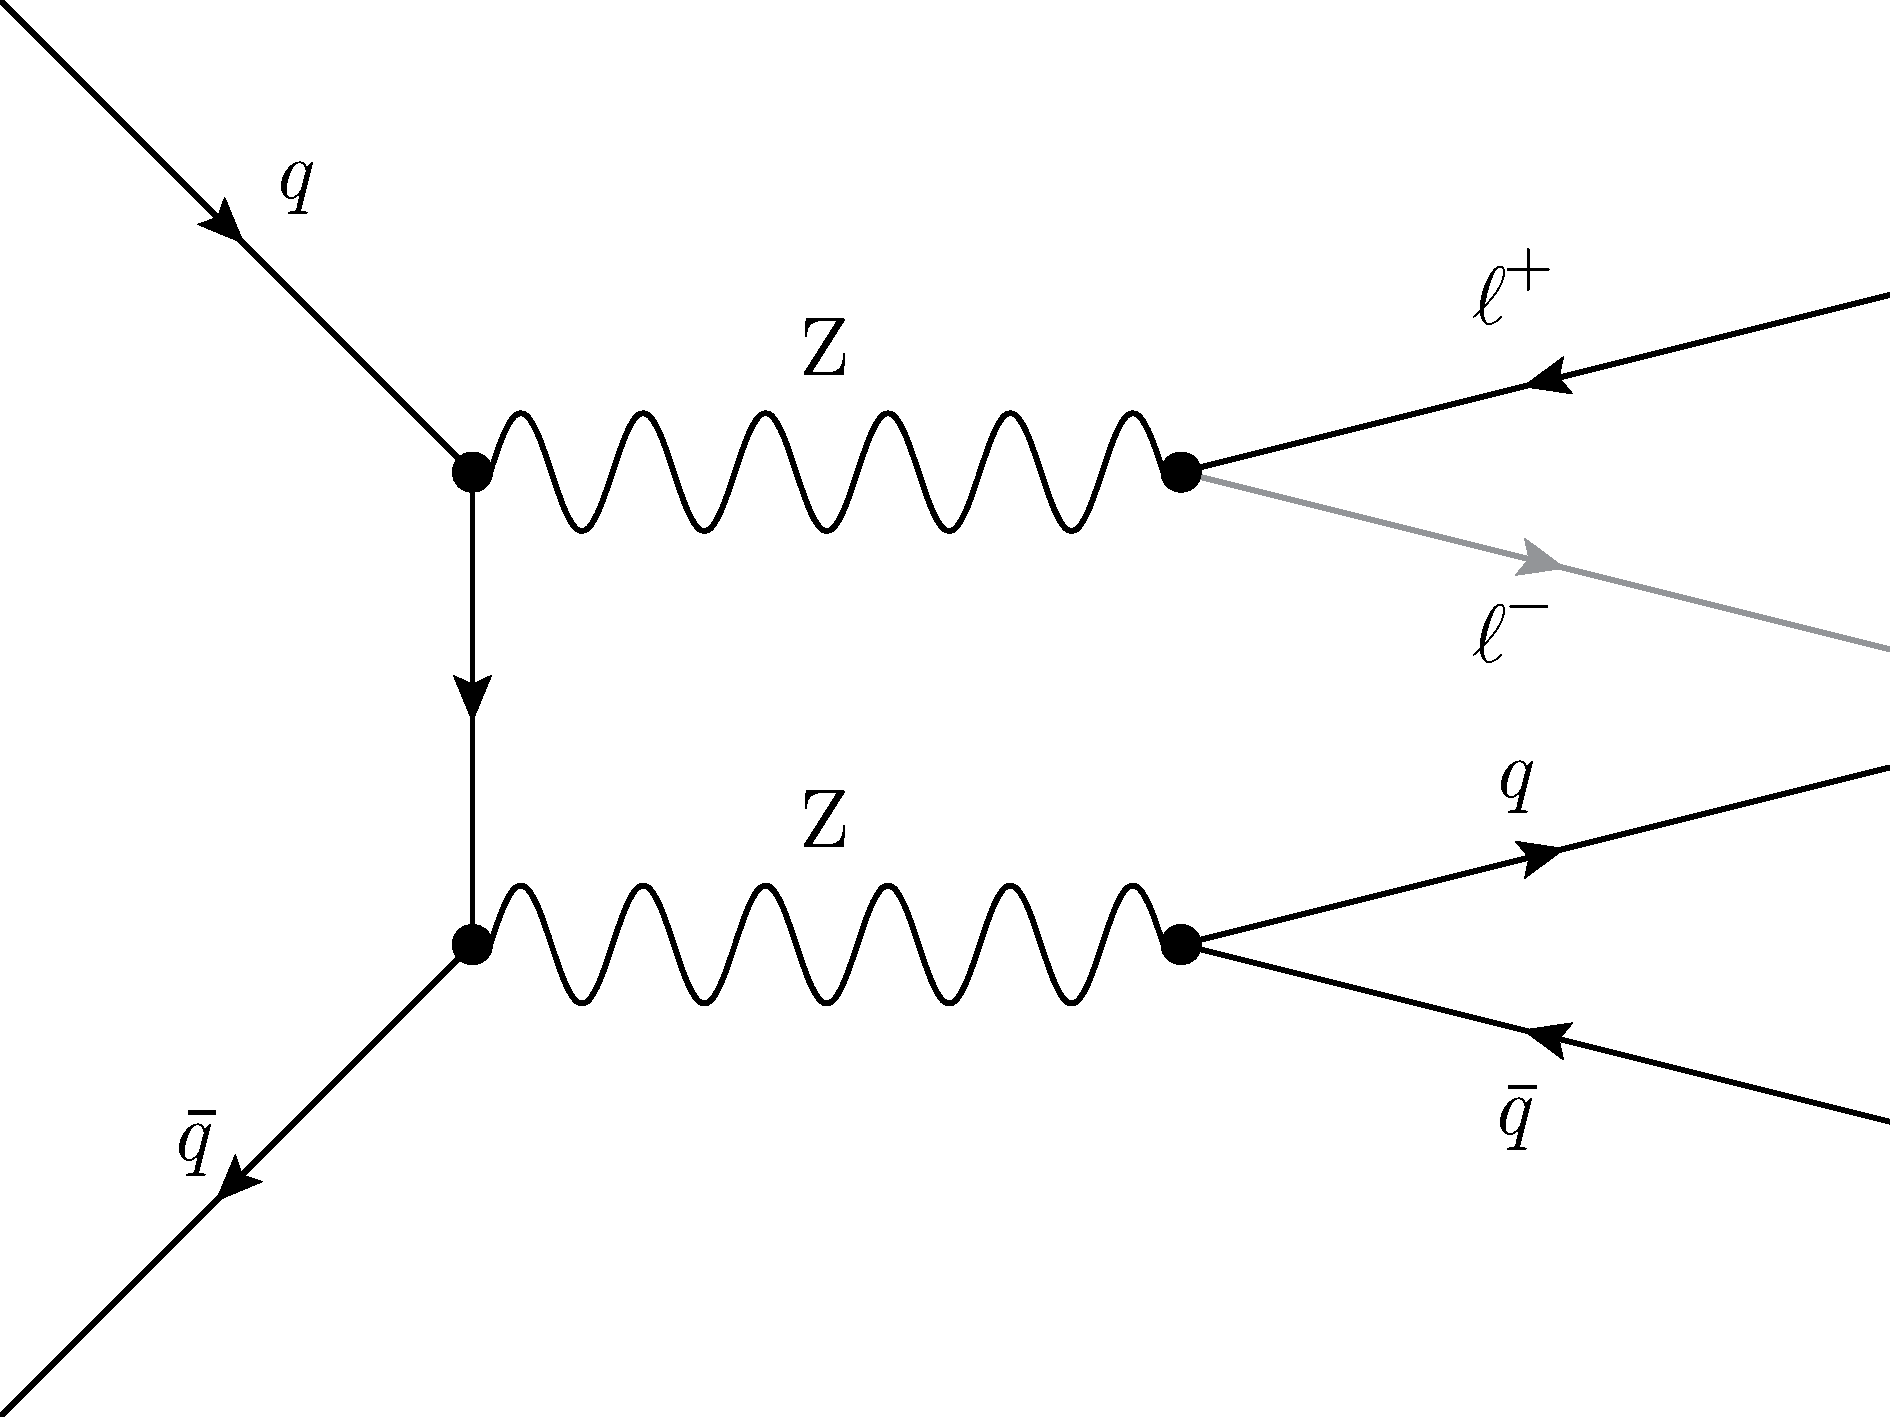
\includegraphics[width=0.25\textwidth]{\figpath/FeynmanDiagrams/ZZ.pdf} \\
			Single-\cPqt\\(\cPqs-channel) & 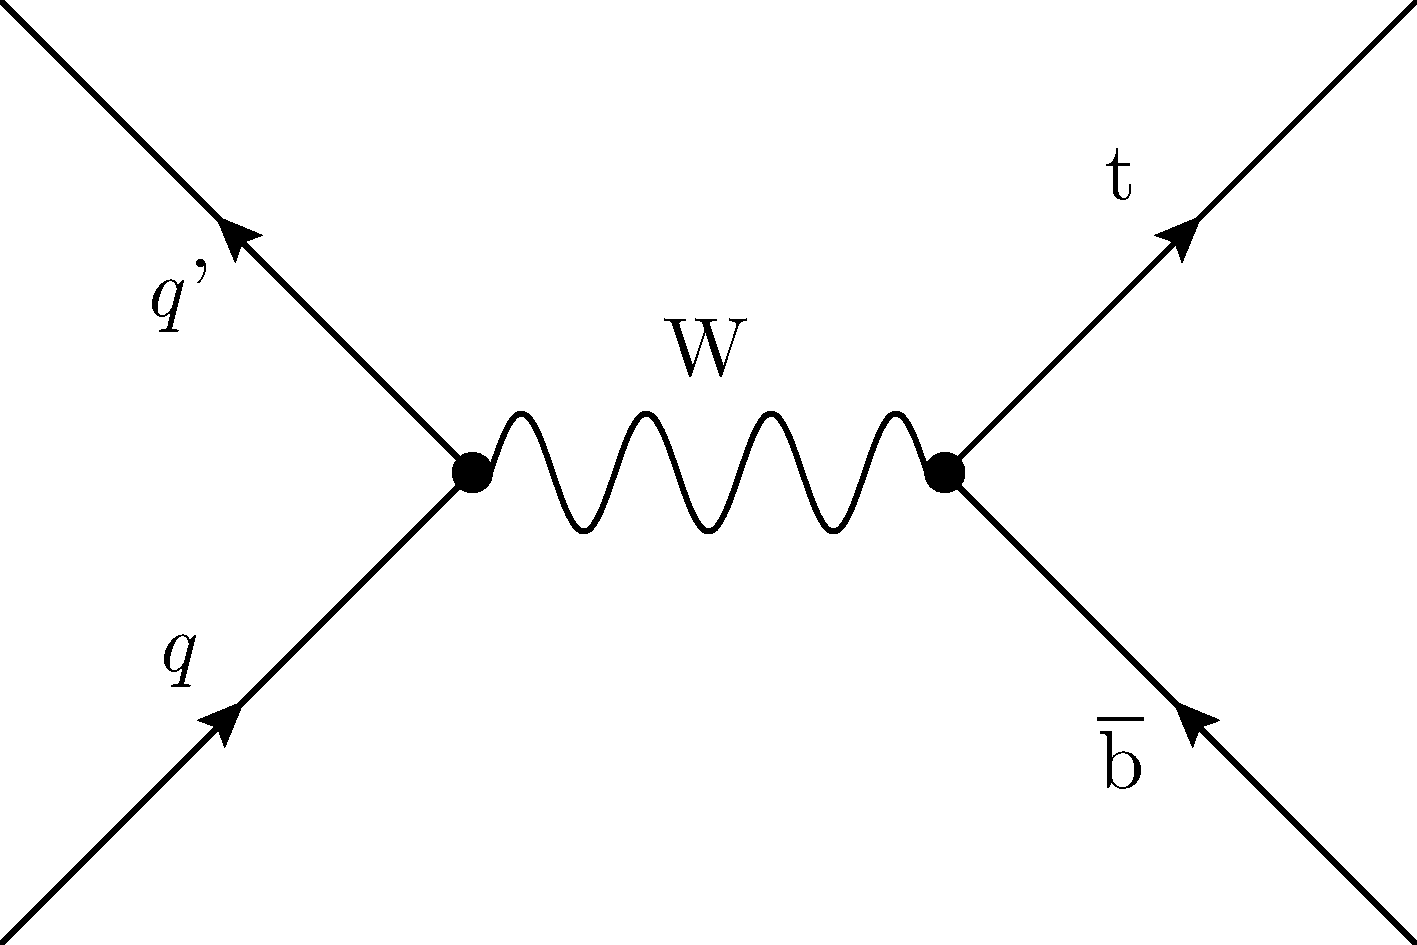
\includegraphics[width=0.25\textwidth]{\figpath/FeynmanDiagrams/STopS.pdf} & Single-\cPqt\\(\cPqt-channel) & 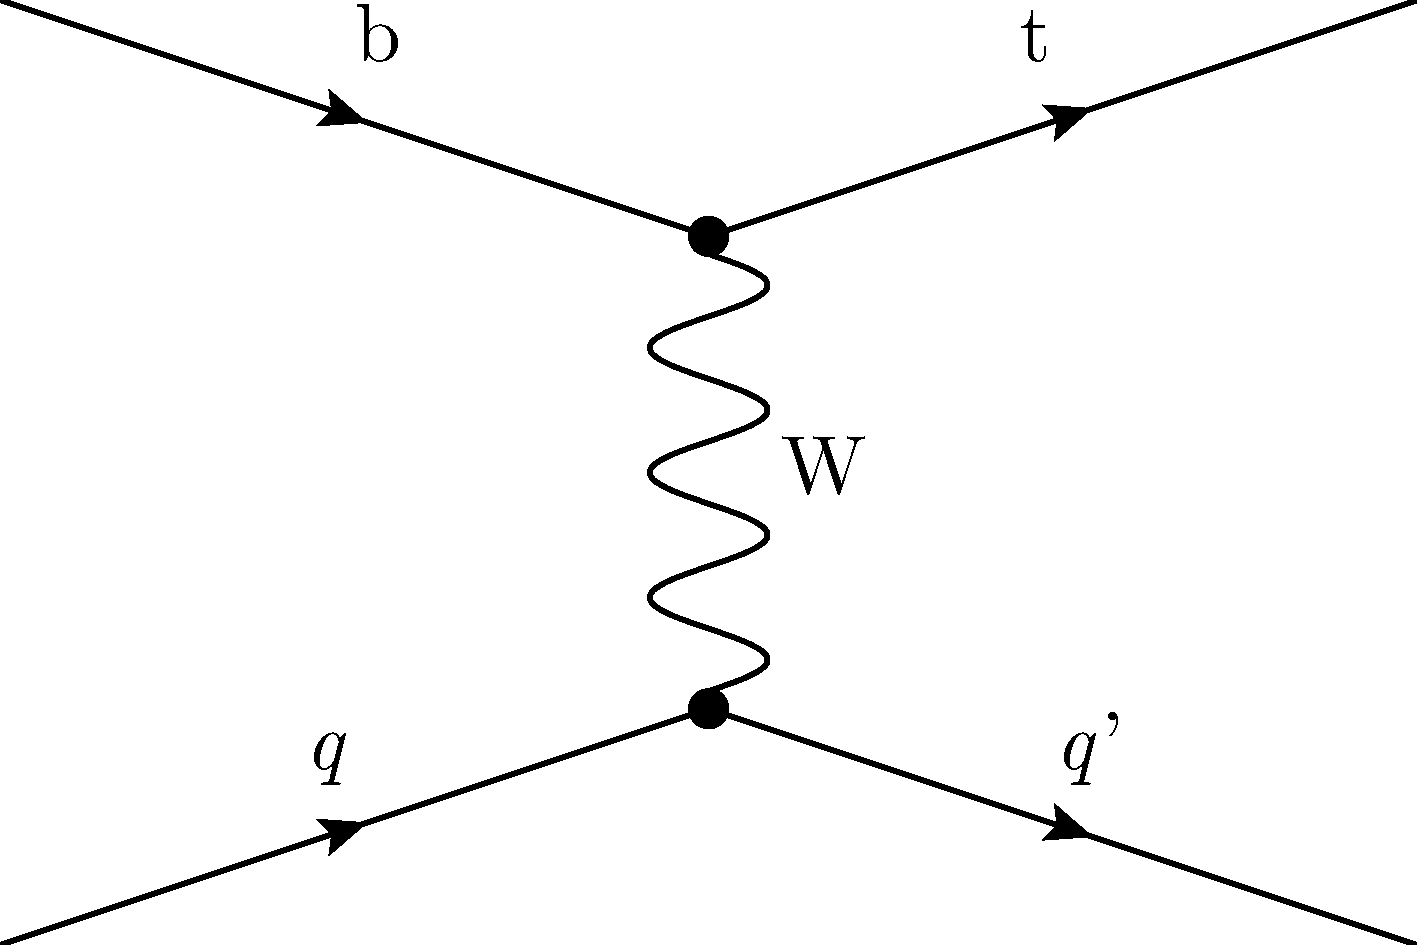
\includegraphics[width=0.25\textwidth]{\figpath/FeynmanDiagrams/STopT.pdf} \\
			Single-\cPqt\\(\cPqt\PW-channel) & 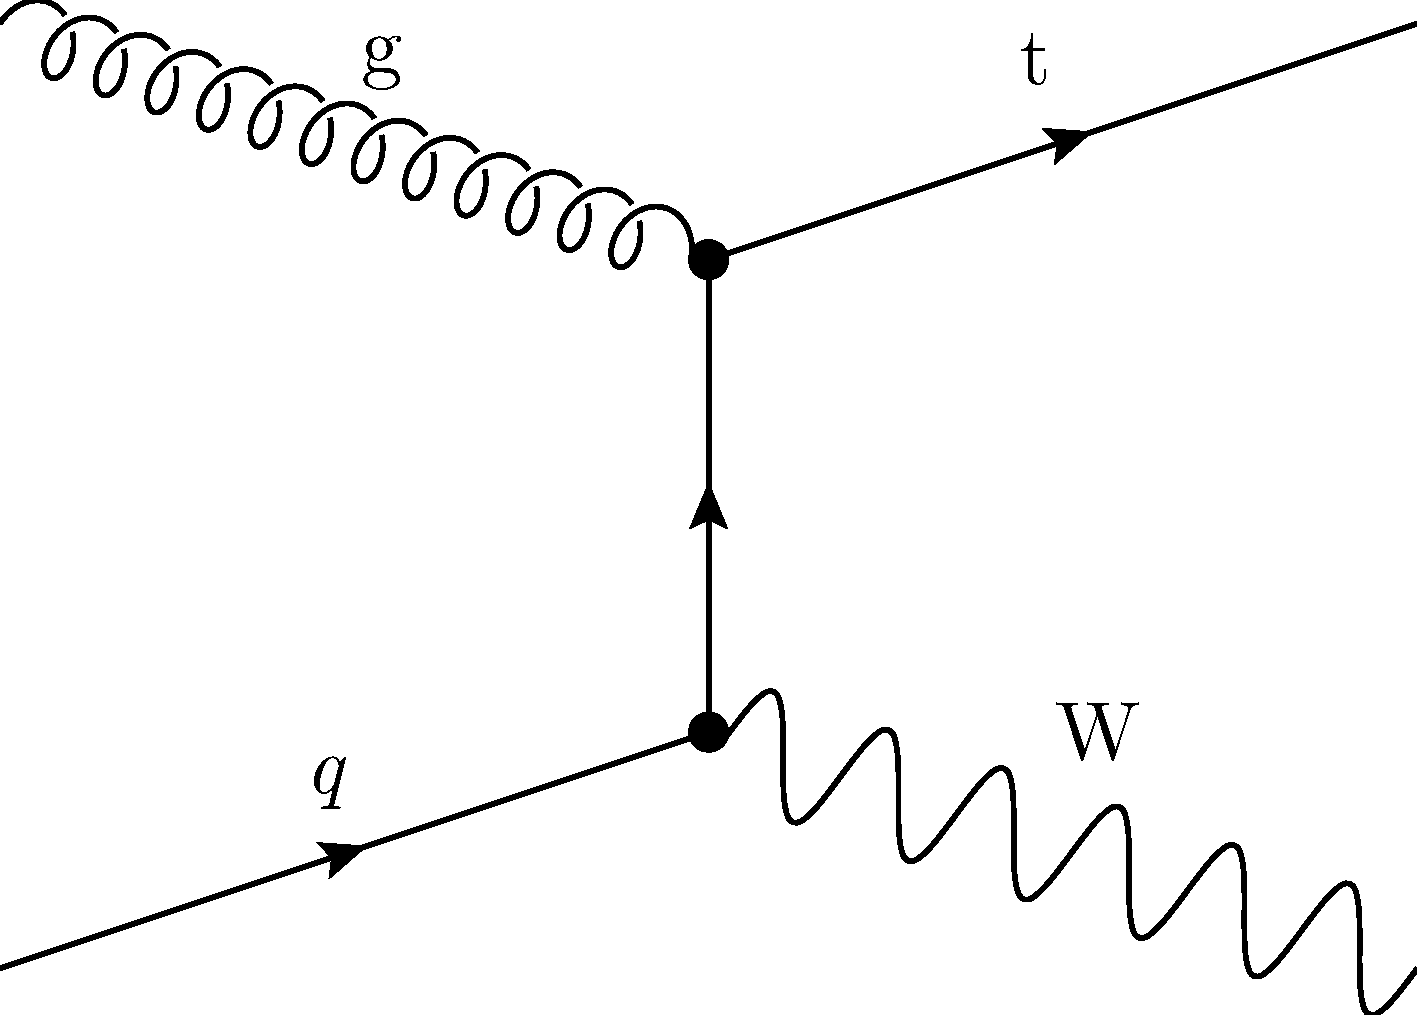
\includegraphics[width=0.25\textwidth]{\figpath/FeynmanDiagrams/STopTW.pdf} & QCD & 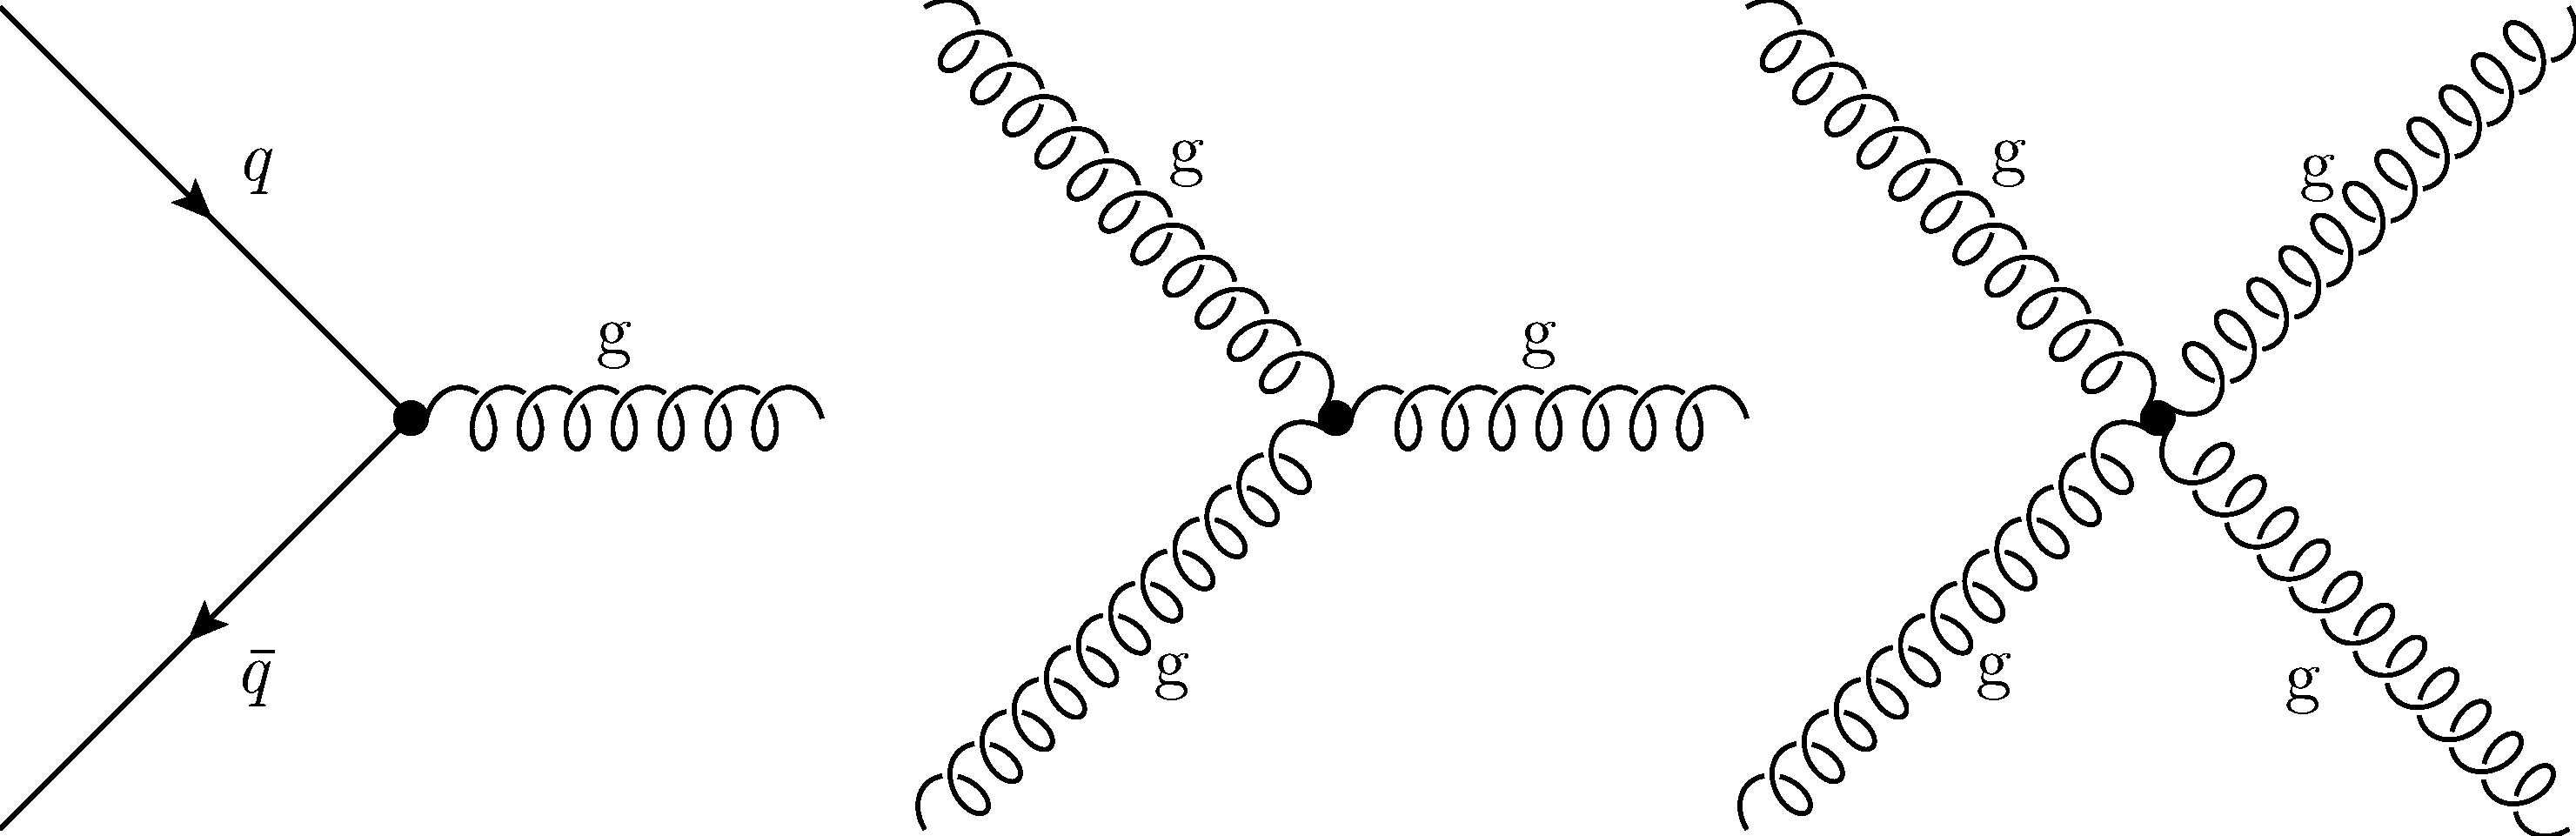
\includegraphics[width=0.25\textwidth]{\figpath/FeynmanDiagrams/QCD.pdf}\\
		\end{tabular}
	\end{table}
\end{frame}

\addtocontents{toc}{\vskip 0.5cm}
\section[Bkg. Est.]{Background Estimation}
\label{sec:background_estimation}
%!TEX root = ../DissertationDefensePresentation.tex

%%--------------------------------------------------------------------------------------------

\subsection*{MC Corrections}

%%--------------------------------------------------------------------------------------------

\begin{frame}
	\frametitle{MC Corrections}
	\framesubtitle{Pileup Reweighting}
	\vspace*{-0.24cm}
	\begin{block}{}
		\begin{itemize}
			\small
			\item MC samples generated using the 2012 assumed pileup scenario
			\item The number of true pileup interactions ($\mu$) is reweighted to match the distribution expected in data
		\end{itemize}
	\end{block}
	\begin{figure}
		\centering
		\begin{subfigure}[t]{0.32\textwidth}
			\includegraphics[width=\textwidth]{\anpath/dataPUdist.png}
		\end{subfigure}
		\begin{subfigure}[t]{0.32\textwidth}
			\includegraphics[width=\textwidth]{\anpath/MCPUdist.png}
		\end{subfigure}
		\begin{subfigure}[t]{0.32\textwidth}
			\includegraphics[width=\textwidth]{\anpath/Weights.png}
		\end{subfigure}
	\end{figure}
	\begin{textblock}{0.2}(0.32,0.50){\color{red}$\div$}\end{textblock}
	\begin{textblock}{0.2}(0.645,0.50){\color{blue}$=$}\end{textblock}
	\vspace*{-0.30cm}
	\begin{figure}
		\centering
		\begin{subfigure}[t]{0.32\textwidth}
			\includegraphics[width=\textwidth]{\figpath/vertices.png}
		\end{subfigure}
		\begin{subfigure}[t]{0.32\textwidth}
			\includegraphics[width=\textwidth]{\figpath/nPV_noRW__comblep_trim.png}
		\end{subfigure}
		\begin{subfigure}[t]{0.32\textwidth}
			\includegraphics[width=\textwidth]{\figpath/nPV__comblep_trim.png}
		\end{subfigure}
	\end{figure}
	\begin{textblock}{0.2}(0.655,0.85){\color{Orange}$\Rightarrow$}\end{textblock}
	\begin{textblock}{0.35}(0.46,0.69){\color{Orange}\Large{Before}}\end{textblock}
	\begin{textblock}{0.35}(0.79,0.69){\color{Orange}\Large{After}}\end{textblock}
\end{frame}

\begin{frame}
	\frametitle{MC Corrections}
    \framesubtitle{Jet Corrections}
    \vspace*{-0.24cm}
    \begin{block}{Jet Energy Corrections}
    	\begin{itemize}
	    	\footnotesize
    		\item Corrects the scale of jets due to pileup and detector effects
    		\item L1FastJet (pileup), L2Relative ($\eta$ dependent), and L3Absolute ($p_{T}$ dependent) corrections
    		\item L2L3Residual (MC/data) corrections used on data only
    	\end{itemize}
    \end{block}
    \vspace*{1.4cm}
    \begin{block}{Jet Energy Resolution}
    	\begin{itemize}
    		\footnotesize
    		\item Deterministic $\eta$-dependent corrections for jets and $\Em_{T}$
    		\item Multiplicative correction factor follows the form shown below
    	\end{itemize}
    \end{block}
    \vspace*{-0.50cm}
    \begin{columns}[T]
    	\begin{column}{0.27\textwidth}
    		\begin{block}{JER Constants}
    			\tiny
    			\begin{table}[ht]
					\centering
					\begin{tabular}{| l | l |}
						\hline\hline\\[-2.75ex]
						$\eta$ &JER Correction\\
						\hline\\[-2.75ex]
						$<0.5$ & $1.052$\\
						\hline\\[-2.75ex]
						$\geqslant0.5\&<1.1$ & $1.057$\\
						\hline\\[-2.75ex]
						$\geqslant1.1\&<1.7$ & $1.096$\\
						\hline\\[-2.75ex]
						$\geqslant1.7\&<2.3$ & $1.134$\\
						\hline\\[-2.75ex]
						$\geqslant2.3\&<5.0$ & $1.288$\\
						\hline\hline
					\end{tabular}
					\label{tab:jer}
					\vspace*{-0.3cm}
				\end{table}
			\end{block}
    	\end{column}
    	\begin{column}{0.32\textwidth}
    		\begin{block}{JER Correction}
    			\Tiny
    			\begin{equation}
				\label{eq:C_JER}
				C_{JER}=max\left(0.0,\frac{p_{T}^{GEN}}{p_{T}^{RECO}}+C_{\eta}\cdot\left(1-\frac{p_{T}^{GEN}}{p_{T}^{RECO}}\right)\right)
				\end{equation}
				\begin{equation}
				\label{eq:Jet_JER}
				Jet_{\textbf{X}}^{corrected}=C_{JER}{\cdot}Jet_{\textbf{X}}^{RECO}
				\end{equation}
    		\end{block}
    	\end{column}
    	\begin{column}{0.34\textwidth}
    		\begin{block}{Propogate to $\Em_{T}$}
    			\tiny
    			\begin{equation}
				\Em_{x}^{corrected}=\left(1-C_{JER}\right)Jet_{x}^{RECO}+{\Em_{T}}_{x}^{RECO}\label{eq:MET_JER_X}
				\end{equation}
				\begin{equation}
				\Em_{y}^{corrected}=\left(1-C_{JER}\right)Jet_{y}^{RECO}+{\Em_{T}}_{y}^{RECO}\label{eq:MET_JER_Y}
				\end{equation}
    		\end{block}
    	\end{column}
    \end{columns}
	\begin{textblock}{1.0}(0.07,0.325)
		\begin{figure}
			\centering
			\scalebox{0.6}{\input{JEC_levels}}
			\label{fig:factorized_approach}
		\end{figure}
	\end{textblock}
\end{frame}

\begin{frame}%<1>[label=frame:event_selection_met_phi]
	\frametitle{MC Corrections}
	\framesubtitle{$\Em_{\phi}$ Reweighting}
	\vspace*{-0.54cm}
	\begin{columns}[T]
		\begin{column}{0.52\textwidth}
			\begin{block}{}
				\begin{itemize}
					\item Clear modulation in the $\Em_{\phi}$ distributions for both data and MC
					\item In 2012 this was peramterized in terms of NPV
					\item $\Em_{\phi}$ correction follows the equations below
				\end{itemize}
%				\vspace*{-0.15cm}
				\begin{equation}
				\Em_{x}^{corrected}=\Em_{x}^{RECO}-\left([0]+[1]{\cdot}nPV\right)\label{eq:METPhi_cor_x}
				\end{equation}
				\begin{equation}
				\Em_{y}^{corrected}=\Em_{y}^{RECO}-\left([0]+[1]{\cdot}nPV\right)\label{eq:METPhi_cor_y}
				\end{equation}
				\vspace*{-0.55cm}
				\begin{table}[hbtp]\footnotesize
					\centering
					\begin{tabular}{|c|c|l|}
					\hline\hline
					Sample & Parameter 0 & Parameter 1 \\
					\hline
					\textbf{Data} & & \\
					x & $2.0105E-01$ & $4.2663E-01$ \\
					\hline
					y & $-9.1350E-01$ & $-2.3120E-01$ \\
					\hline\hline
					\textbf{MC} & & \\
					x & $2.9059E-01$ & $-3.5293E-03$ \\
					\hline
					y & $3.0183E-01$ & $-1.9974E-01$ \\
					\hline\hline
					\end{tabular}
					\label{tab:METPhi_cor_xy}
				\end{table}
			\end{block}
		\end{column}
		\begin{column}{0.45\textwidth}
			\begin{figure}
				\centering
				\begin{subfigure}[t]{\textwidth}
					\only<1>{\includegraphics[width=\textwidth]{\anpath/METPhi_Before-eps-converted-to.pdf}}
					\only<2>{\includegraphics[width=\textwidth]{\anpath/METPhi_After-eps-converted-to.pdf}}
				\end{subfigure}
				\newline
				\begin{subfigure}[t]{\textwidth}
					\only<1>{\includegraphics[width=\textwidth]{\anpath/METxyVsNPV_Before-eps-converted-to.pdf}}
					\only<2>{\includegraphics[width=\textwidth]{\anpath/METxyVsNPV_After-eps-converted-to.pdf}}
				\end{subfigure}
			\end{figure}
		\end{column}
	\end{columns}
\end{frame}
%\againframe<2>{frame:event_selection_met_phi}

\begin{frame}
	\frametitle{MC Corrections}
	\framesubtitle{$p_{T}^{Top}$ Reweighting}
	\vspace*{-0.34cm}
	\begin{columns}[T]
		\begin{column}{0.5\textwidth}
			\begin{block}{}
				\begin{itemize}
					\item The top quark $p_{T}$ spectrum in data is softer than found in the NNLO predictions
					\item Right: Fit of $p_{T}^{Top}$ for data/MC in multiple analysis regimes
					\item Top weights were derived as a function of the generated $p_{T}$ of the top quark pair
					\begin{itemize}
						\item Correction only applied to TTbar sample where there exists a top quark pair
					\end{itemize}
				\end{itemize}
				\begin{equation}\label{eq:ttbar_weight_1}
				Weight=\sqrt{SF\left(t\right)SF\left(\bar{t}\right)}
				\end{equation}
				\begin{equation}\label{eq:ttbar_weight_2}
				SF\left(x\right)=e^{a+b{\cdot}x}
				\end{equation}
				\begin{equation}\label{eq:ttbar_weight_2}
				x=p_{T}\text{, }a=0.159\text{, }b=-0.00141
				\end{equation}
			\end{block}
		\end{column}
		\begin{column}{0.46\textwidth}
			\vspace*{0.5cm}
			\begin{figure}
				\centering
				\includegraphics[width=\textwidth]{\figpath/TopPt_Data_MC}
			\end{figure}
		\end{column}
	\end{columns}

\end{frame}

%%--------------------------------------------------------------------------------------------

\subsection*{QCD Model}

%%--------------------------------------------------------------------------------------------
\begin{frame}
	\frametitle{Data-Driven QCD Model}
	\vspace*{-0.24cm}
	\begin{block}{}
		\begin{itemize}
			\small
			\item The QCD multijet background:
			\begin{itemize}
				\footnotesize
				\item Hard to model because of the non-perturbative nature of QCD
				\item Few MC events pass our selection criteria even though the MC samples are large
			\end{itemize}
			\item Data-driven technique:
			\begin{itemize}
				\footnotesize
				\item Make use of the full 2012 single lepton datasets (same datasets mentioned before)
				\item Selection criteria ensures that the events are orthogonal to the data selection
			\end{itemize}
		\end{itemize}
	\end{block}
	\vspace*{-0.49cm}
	\begin{columns}[T]
		\column{0.48\textwidth}
			\vspace*{-0.1cm}
			\begin{center}
				\includegraphics[width=0.9\textwidth]{\figpath/pfIsoVsEta_Full.png}
			\end{center}
		\column{0.49\textwidth}
			\begin{block}{Selection Criteria}
				\begin{itemize}
					\scriptsize
					\item Our QCD sample is obtained from the anti-isolated lepton region (antiIso)
					\vspace*{-0.15cm}
					\item Electrons:
					\begin{itemize}
						\scriptsize
						\item Drop MVA ID requirement
						\item PF Isolation: $<0.2{\rightarrow}>0.3$
					\end{itemize}
					\vspace*{-0.25cm}
					\item Muons:
					\begin{itemize}
						\scriptsize
						\item PF Isolation: $<0.12{\rightarrow}>0.2$
					\end{itemize}
				\end{itemize}
			\end{block}
			\vspace*{-0.30cm}
			\begin{block}{}
				\begin{enumerate}
					\scriptsize
					\item Must PU reweight as $N_{PV}$ distribution different in antiIso region than in SR (selection bias)
					\vspace*{-0.1cm}
					\item Ratio of events in signal region to anti-isolated region varies as a function of $\eta$ (studied in MC)
					\begin{itemize}
						\scriptsize
						\item Transform expected yields to match SR by fitting the $\Em_{T}$ distributions of QCD and \Wjets to data
					\end{itemize}
				\end{enumerate}
			\end{block}
	\end{columns}

	\begin{textblock}{0.5}(0.01,0.93)
		\scriptsize 1.09\% contamination from non-QCD events
	\end{textblock}
\end{frame}

\begin{frame}
	\frametitle{Data-Driven QCD Model}
	\framesubtitle{Methodology}
	\vspace*{-0.24cm}
	\begin{columns}[T]
		\begin{column}{0.49\textwidth}
			\vspace*{-0.3cm}
			\begin{block}{Shape}
				\vspace*{-0.35cm}
				\begin{aeq}{eq:N_QCD_sig}
					N_{SR}^{QCD}\left(\eta\right)=N_{antiIso}^{QCD}\left(\eta\right){\cdot}s^{QCD}\left(\eta\right)
				\end{aeq}
				\vspace*{-0.35cm}
				\begin{itemize}
					\footnotesize
					\item $N_{antiIso}^{QCD}$ and $N_{SR}^{QCD}$ are the number of QCD events in the antiIso and SR for a given luminosity
					\item $s^{QCD}$: transfer weight obtained from fit{\tikz[remember picture]{\node[coordinate] (s-fit) {};}}
					\item \Wjets (biggest background) and QCD have differently shaped $\Em_{T}$ distributions
				\end{itemize}
			\end{block}
			\vspace*{-0.25cm}
			\begin{block}{Normalization over all $\eta$}
				\begin{itemize}
					\footnotesize
					\item Determine the QCD \& \Wjets event yields (global scale factor):
					\begin{itemize}
						\footnotesize
						\item Fit to the $\Em_{T}$ distribution with all $\eta$ bins combined
						\item Done in the $\geqslant2$ jets bin
						\item The fit gives us the QCD normalization and a scale factor for \Wjets (very close to 1)
					\end{itemize}
				\end{itemize}
			\end{block}
		\end{column}
		\begin{column}{0.48\textwidth}
			\begin{tikzpicture}[remember picture]
				\node [inner sep=0pt,above right] {\includegraphics[width=\textwidth]{\figpath/SingleMetFit_control6_electron_crop.pdf}};
				\node[anchor=base] (fit) at (1.2,3) {};
			\end{tikzpicture}
			\begin{table}[ht]
				\caption{\scriptsize{Absolute scale factors for the \Wjets and QCD samples in the electron and muon channels}}
				\centering
				\scriptsize
				\begin{tabular}{| l | c | r |}
					\hline\hline\\[-2.7ex]
					& Electrons & Muons\\
					\hline\\[-2.7ex]
					WJets & $1.045\pm0.005$ & $0.970\pm0.004$\\
					\hline\\[-2.7ex]
					QCD & $0.249\pm0.013$ & $0.145\pm0.007$\\
					\hline
				\end{tabular}
				\label{tab:yields}
			\end{table}
		\end{column}
	\end{columns}
	\begin{textblock}{0.25}(0.83,0.38)
		1 jet CR
	\end{textblock}
	\begin{textblock}{0.25}(0.70,0.25)
		\color{red} Floating
	\end{textblock}
	\begin{textblock}{0.25}(0.70,0.285)
		\color{green} Floating
	\end{textblock}
	\begin{textblock}{0.25}(0.70,0.32)
		\color{blue} Fixed
	\end{textblock}
	\begin{tikzpicture}[overlay]
			\path[->,violet,thick] ([xshift=1mm,yshift=1mm]s-fit) edge [out=0,in=180] (fit);
	\end{tikzpicture}
\end{frame}

\begin{frame}<1>[label=frame:qcd_model_normalization]
	\frametitle{Data-Driven QCD Model}
	\framesubtitle{Final Product}
	\vspace*{-0.24cm}
		\begin{textblock}{0.50}(0.25,0.12)
			\begin{center}
				\includegraphics[width=0.95\textwidth]{\figpath/MET_electron.png}
			\end{center}
		\end{textblock}
		\begin{textblock}{0.50}(0.45,0.40)
			{\color{orange}\Large Excellent\\Agreement!}
		\end{textblock}
\end{frame}

%%--------------------------------------------------------------------------------------------

\subsection*{Validation}

%%--------------------------------------------------------------------------------------------

\begin{frame}
	\frametitle{Kinematic Validation Plots}
	\framesubtitle{2 Jets - Muon Bin}
	\begin{block}{}
		\begin{itemize}
			\item Some relevant distributions shown here
			\begin{itemize}
			 	\item Good agreement in all distributions
			 	\item Similar agreement for muons and other jet bins 
			 \end{itemize}
		\end{itemize}
	\end{block}
	\vspace*{-0.24cm}
	\begin{columns}[T]
		\column{0.31\textwidth}
			\begin{block}{\scriptsize \Mjj}
				\includegraphics[width=\textwidth]{\figpath/Mjj_muon_2jets.pdf}%
			\end{block}
		\column{0.31\textwidth}
			\begin{block}{\scriptsize \Mlv}
				\includegraphics[width=\textwidth]{\figpath/WmT_muon_2jets.pdf}%
			\end{block}
		\column{0.31\textwidth}
			\begin{block}{\scriptsize \Mlvjj}
				\includegraphics[width=\textwidth]{\figpath/Mlvjj_muon_2jets.pdf}%
			\end{block}
	\end{columns}
\end{frame}

%%--------------------------------------------------------------------------------------------

\subsection*{Yields}

%%--------------------------------------------------------------------------------------------

\begin{frame}
	\frametitle{Expected Yields}
	\begin{itemize}
		\item Table of expected yields split by jet category (2, 3, or $\geqslant$4) for the combined lepton category ($\Pe+\Pmu$)
	\end{itemize}
	\begin{table}[htbp]
		\color{black}
		\centering
		\scriptsize
		\label{tab:NoBTagYield}
		\begin{tabular}{|p{3.5cm}|c|c|c|} \hline
			\textbf{Process} & \textbf{2 Jets} & \textbf{3 Jets} & \textbf{$\geqslant$4 Jets}\\ \hline
			Diboson & $46495.97\pm78.55$ & $15049.18\pm44.70$ & $4150.48\pm23.47$ \\
			\rowonly<2>{\rowcolor{ForestGreen}}
			\Wjets & $3446003.06\pm6434.30$ & $756463.35\pm3008.63$ & $189815.29\pm1515.40$ \\
			\Zjets & $270460.62\pm822.24$ & $69061.73\pm415.90$ & $19829.24\pm222.71$ \\
			\ttbar & $22452.06\pm142.85$ & $27902.44\pm160.86$ & $31218.33\pm170.54$ \\
			Single \cPqt & $16587.13\pm84.31$ & $7193.89\pm59.29$ & $3068.60\pm40.25$ \\
			Multijet & $275465.33\pm952.52$ & $74168.89\pm504.39$ & $22109.53\pm282.94$ \\\hline
			\rowtemporal<2>{\rowcolor{mygray}}{\rowcolor{ForestGreen}}{\rowcolor{mygray}}
			Total Background & $4077464.17\pm6558.75$ & $949839.48\pm3083.93$ & $270191.47\pm1567.59$ \\\hline
			\ggH, \HWW \MH=125\gev & $552.09\pm1.92$ & $211.15\pm1.19$ & $79.51\pm0.73$ \\
			\qqH, \HWW \MH=125\gev & $106.60\pm0.56$ & $52.66\pm0.39$ & $17.51\pm0.23$ \\
			\WH\_\ZH\_\ttH \newline \HWW \MH=125\gev & $136.20\pm2.22$ & $84.35\pm1.75$ & $42.32\pm1.22$ \\\hline
			\rowtemporal<3>{\rowcolor{mygray}}{\rowcolor{Mulberry}}{\rowcolor{mygray}}
			Total \HWW & $794.89\pm2.99$ & $348.16\pm2.15$ & $139.34\pm1.44$ \\\hline
			\WH\_\ZH\_\ttH \newline \HZZ \MH=125\gev & $10.30\pm0.17$ & $5.30\pm0.12$ & $2.35\pm0.08$ \\
			\WH, \Hbb \MH=125\gev & $45.34\pm0.40$ & $14.22\pm0.23$ & $3.86\pm0.12$ \\
			\ttH, \Hbb \MH=125\gev & $0.59\pm0.03$ & $1.33\pm0.05$ & $3.77\pm0.09$ \\\hline
			\rowcolor{mygray}
			Total Volunteer Signal & $56.23\pm0.44$ & $20.85\pm0.26$ & $9.98\pm0.17$ \\\hline
			\rowonly<4>{\rowcolor{red}}
			Signal \textsubscript{\HWW}/Bkg & 0.000195 & 0.000367 & 0.000516 \\
			Signal \textsubscript{\HWW}/$\sqrt{\text{Bkg}}$ & 0.394 & 0.357 & 0.268 \\\hline
			\rowcolor{mygray}
			Data & $4057594$ & $953513$ & $272713$ \tabularnewline\hline
		\end{tabular}
	\end{table}
	\begin{itemize}
		\item \only<4>{\color{red}}The background is $\sim5000$ times bigger than the signal
	\end{itemize}
\end{frame}

\addtocontents{toc}{\vskip 0.5cm}
\section[MVA]{Signal Discrimination Techniques}
\label{sec:mem}
%!TEX root = ../DissertationDefensePresentation.tex

{
\usebackgroundtemplate{
  
\begin{tikzpicture}
    \path [outer color = white, inner color = gray!85]
      (0,0) rectangle (\paperwidth,\paperheight);
  \end{tikzpicture}}
\begin{frame}
	\begin{textblock}{1.0}(0.00,0.20)
        \begin{tcbraster}[raster columns=2,raster force size=false,size=fbox]
            \begin{center}
                \tcbincludegraphics[blank,arc=0.3cm,hbox,graphics options={width=0.5\textwidth}]{\figpath/mem.png}\hspace*{0.1cm}\tcbincludegraphics[blank,arc=\ClipSep,hbox,graphics options={width=0.3\textwidth}]{\figpath/decision_tree.png}
            \end{center} 
        \end{tcbraster}
    \end{textblock}
    \begin{textblock}{1.0}(0.0,0.75)
    	\color{black}
        \begin{center}
            \Huge
            Signal Extraction\\
            \large
            Templates, Marix Element Methods, and Boosted Decision Trees
        \end{center}
    \end{textblock}
\end{frame}
}

%%--------------------------------------------------------------------------------------------

\subsection*{Matrix Element Method}

%%--------------------------------------------------------------------------------------------

\begin{frame}%<1>[label=frame:MEM_formalism]
	\frametitle{Matrix Element Analysis}
	\framesubtitle{Formalism}
	\vspace*{-0.24cm}
	\footnotesize
	\begin{block}{Problem:}
	\begin{itemize}
		\item Many template based analyses/BDTs ignore much of the event information, instead using a few discriminating distributions
		\begin{itemize}
			\footnotesize
			\item Can miss important distributions as these analyses often rely on shallow networks, which are bad at finding non-linear functions
		\end{itemize}
	\end{itemize}
	\end{block}
	\vspace*{-0.24cm}
	\begin{block}{Solution:}
		\begin{itemize}
			\scriptsize
			\item The Matrix Element Method (MEM) takes into account all final state particle kinematics and correlations
			\item MEMs give an estimate, probability density $P_{i}$, that an event with a given final state comes from process $i$
		\end{itemize}
		\vspace*{-0.15cm}
		\only<1> {
			\begin{center}
				\includegraphics[width=0.5\textwidth]{\figpath/ggH_new.pdf}
			\end{center}
		}
		\only<2> {
			\begin{center}
				\includegraphics[width=0.5\textwidth]{\figpath/WJets1_new.pdf}
			\end{center}
		}
		\only<3-> {
		\begin{equation}\label{eq:MEM_probability}
%P_{sig}\left(x,m_{H}\right)=\frac{1}{N}\int_{y,q_{1},q_{2}}d\Phi\left(y\right)|M_{ggH}\left(y,m_{H}\right)|^{2}W\left(x,y\right)f_{pdf}\left(q_{1}\right)f_{pdf}\left(q_{2}\right)dq_{1}d1_{2}\\
{\color<8>{red}P_{i}}={\int}{\color<6>{red}T\left(\mathbf{X};\mathbf{Y}\right)}\frac{1}{\sigma_{i}}\sum_{flavor}\int_{V_{n}}{\color<4>{red}\mathcal{M}_{i}^{2}}\left(\mathbf{Y}\right)\frac{{\color<5>{red}f_{1}\left(q_{1},Q^{2}\right)f_{2}\left(q_{2},Q^{2}\right)}}{|\vec{q}_{1}|\cdot|\vec{q}_{2}|}{\color<7>{red}d\Phi_{n}\left(q_{1}+q_{2};y_{1},...,y_{n}\right)}d\mathbf{Y}
		\end{equation}
		\vspace*{-0.15cm}
		\begin{equation}\label<3>{eq:MEM_phaseSpace}
d\Phi_{n}\left(q_{1}+q_{2};y_{1},...,y_{n}\right)=\left(2\pi\right)^{4}\delta^{4}\left(q_{1}+q_{2}-\sum_{i=1}^{n}y_{i}\right)\prod_{i=1}^{n}\frac{d^{3}y_{i}}{\left(2\pi\right)^{3}2E_{i}}
		\end{equation}
		\vspace*{-0.15cm}
		\begin{itemize}
			\scriptsize
			\uncover<4->{\item $\mathcal{M}_{i}$ is the matrix element for the $2{\rightarrow}n$ process $i$}
			\uncover<5->{\item $f_{1}$ and $f_{2}$ are the PDF for the colliding partons $q_{1}$ and $q_{2}$ with beam energy fractions $x_{1}$ and $x_{2}$}
			\uncover<6->{\item $T\left(\vec{x},\vec{y}\right)$ is the transfer function, which maps the measured jet energies to the possible parton energies}
			\uncover<7->{\item $d\Phi$ (equation~\ref{eq:MEM_phaseSpace}) is the n-body phase space term}
			\uncover<8->{\item For each event we evaluate $P_{i}$ for 15 different processes}
		\end{itemize}
		}
	\end{block}
\end{frame}
%\againframe<2>{frame:MEM_formalism}
%\againframe<3>{frame:MEM_formalism}
%\againframe<4>{frame:MEM_formalism}
%\againframe<5>{frame:MEM_formalism}
%\againframe<6>{frame:MEM_formalism}
%\againframe<7>{frame:MEM_formalism}
%\againframe<8>{frame:MEM_formalism}

\begin{frame}
	\frametitle{Matrix Element Analysis}
	\framesubtitle{Evaluation}
	\vspace*{-0.24cm}
	\begin{block}{Monte Carlo Integration}
		\begin{itemize}
			\item Integration was performed using the \textbf{adaptive quadrature} method in the ROOT software package
			\begin{itemize}
				\item Based upon the CERNLIB RADMUL routine
			\end{itemize}
			\item The integral is computed over N-dimensional rectangular regions to an attempted, user-specified accuracy ($\epsilon$)
		\end{itemize}
		\begin{equation}
			I_{n}=\int_{a_{n}}^{b_{n}}\int_{a_{n-1}}^{b_{n-1}}\ldots\int_{a_{1}}^{b_{1}}f\left(x_{1},x_{2},\ldots,x_{n}\right)dx_{1}dx_{2}{\ldots}dx_{n}
		\end{equation}
		\vspace*{-0.40cm}
		\begin{itemize}
			\item The integration space is iteratively subdivided\\into $B_{i}$ regions
			\begin{itemize}
				\item A region is divided in half, along the axis\\most difficult to integrate, if the error\\within that region is the largest of all regions
				\item This stops when $\epsilon$ is reached
			\end{itemize}
			\item For each rectangular subregion there are\\$2^{n}+2n^{2}+2n+1$ function evaluations
		\end{itemize}
		\vspace*{-0.035cm}
		{\tiny A. van Doren and L. de Ridder, An adaptive algorithm for numerical integration over an n-dimensional cube, J. Comput. Appl. Math. 2 (1976) 207-217.}
	\end{block}
	\begin{textblock}{0.25}(0.68,0.540)
		\includegraphics[width=\textwidth]{\figpath/AdaptiveQuadratureRADMUL.png}
	\end{textblock}
\end{frame}

\begin{frame}
	\frametitle{Matrix Element Analysis}
	\framesubtitle{Computation \& Combination of Probability Densities}
	\vspace*{-0.24cm}

	\begin{block}{MEM Computation}
		\begin{itemize}
			\small
			\item The probabilities are calculated for a total of \textbf{62 processes/masses}
			\begin{itemize}
				\item \textbf{Computation Time}: $\sim12$ million CPU hours
			\end{itemize}
			\item The following 15 are the ones used in this analysis (all 3 dimensional integrations)
		\end{itemize}
		\vspace*{-0.3cm}
		\begin{columns}[T]
			\footnotesize
			\column{0.14\textwidth}
			\begin{itemize}
				\item {\color{red}$\cmsSymbolFace{W}\cmsSymbolFace{W}$}
				\item {\color{red}$\cmsSymbolFace{W}\cmsSymbolFace{Z}$}
				\item {\color{red}$\cmsSymbolFace{W}\cmsSymbolFace{Z}\cPqb\cPqb$}
				\item {\color{red}$\cmsSymbolFace{W}\cmsSymbolFace{L}\cPg$}
			\end{itemize}
			\column{0.27\textwidth}
			\begin{itemize}
				\item {\color{red}$\cmsSymbolFace{W}\cmsSymbolFace{L}\cPg$ (second order)}
				\item {\color{red}$\cmsSymbolFace{W}\cmsSymbolFace{L}\cmsSymbolFace{L}$}
				\item {\color{red}$\cmsSymbolFace{W}\cPg\cPg$}
				\item {\color{red}$\cmsSymbolFace{W}\cmsSymbolFace{L}\cPqb$}
			\end{itemize}
			\column{0.29\textwidth}
			\begin{itemize}
				\item {\color{red}$\cmsSymbolFace{W}\cPqb\cPqb$}
				\item {\color{red}ZLight}
				\item {\color{red}Single Top \cPqs-channel}
				\item {\color{red}Single Top \cPqt-channel}
			\end{itemize}
			\column{0.30\textwidth}
			\begin{itemize}
				\item {\color{red}QCD}
				\item {\color{red}ggH (\MH=125\gev)}
				\item {\color{red}WH (\MH=125\gev)}
			\end{itemize}
		\end{columns}
	\end{block}
	\vspace*{-0.24cm}
	\begin{block}{We still needed to combine the 15 MEs into some discriminator}
	 	\begin{itemize}
	 		\item Could have followed the CDF Single Top analysis or the CMS $\PH{\rightarrow}\ZZ{\rightarrow}4\ell$ analysis in making use of the Neyman-Pearson lemma to form a ratio of likelihoods
	 		%\begin{itemize}
	 		%	\item In CMS this is called a Matrix Element Likelihood Analysis (MELA)
	 		%\end{itemize}
	 		\item We found this methodology to be inferior to using a \textbf{Boosted Decision Tree (BDT)} classifier
	 		\begin{itemize}
	 			\item This gives a typically shallow networked (BDT) the ability to create a non-linear discriminant function because the inputs are already non-linear variables
	 		\end{itemize}
	 	\end{itemize}
	\end{block}
\end{frame}

\begin{frame}<1>[label=frame:MEM_computation_combination]
	\frametitle{Matrix Element Analysis}
	\framesubtitle{ME BDT Results}
	\vspace*{-0.24cm}
	\begin{textblock}{0.96}(0.0175,0.14)
		\begin{block}{}
			\begin{itemize}
				\item BDT discriminant computed for individual jet bins
				\begin{itemize}
					\item {\color{blue}Blue: Signal}
					\item {\color{red}Red: Background}
				\end{itemize}
			\end{itemize}
		\end{block}
	\end{textblock}
	\begin{textblock}{0.96}(0.0175,0.33)
		\begin{alertblock}{BDT Discriminants}
			\centering
			\includegraphics[width=0.33\textwidth]{\figpath/MVA/2015_07_17_TMVA_output_jets2_eq0tag_both_HToWW_WJets_allEvtProbs_0KinVar/mva_BDT.pdf}%
			\includegraphics[width=0.33\textwidth]{\figpath/MVA/2015_07_17_TMVA_output_jets3_eq0tag_both_HToWW_WJets_allEvtProbs_0KinVar/mva_BDT.pdf}%
			\includegraphics[width=0.33\textwidth]{\figpath/MVA/2015_07_17_TMVA_output_jets4_eq0tag_both_HToWW_WJets_allEvtProbs_0KinVar/mva_BDT.pdf}%
		\end{alertblock}
	\end{textblock}
	\begin{textblock}{0.15}(0.24,0.53){\color{red}{2 Jets}}\end{textblock}
	\begin{textblock}{0.15}(0.56,0.53){\color{red}{3 Jets}}\end{textblock}
	\begin{textblock}{0.15}(0.88,0.53){\color{red}{$\geq$4 Jets}}\end{textblock}
	\begin{textblock}{0.96}(0.0175,0.76)
		\begin{block}{}
			\begin{itemize}
				\item Some discrimination between signal and background
				\begin{itemize}
					\item Tough analysis given the similar kinematics of signal and background
				\end{itemize}
				\item ME is LO only and permutations of jets and partons degrades discrimination
			\end{itemize}
		\end{block}
	\end{textblock}
\end{frame}
\label{sec:signal_extraction}
%!TEX root = ../DissertationDefensePresentation.tex

%%--------------------------------------------------------------------------------------------

\subsection*{Combined Discriminant}

%%--------------------------------------------------------------------------------------------

\begin{frame}
	\frametitle{Matrix Element Analysis}
	\framesubtitle{Improving Sensitivity}
	\vspace*{-0.24cm}
	\begin{columns}[T]
		\begin{column}{0.47\textwidth}
			\vspace*{-0.15cm}
			\begin{block}{}
				\begin{itemize}
					\item We added new kinematic variables to improve the sensitivity
					\item Optimized individually for different jet bins
					\begin{itemize}
						\item Background compositions different in each bin
					\end{itemize}
					\item Looked at 46 variables and identified the most discriminating
					\begin{itemize}
						\item Iterative process: a subset was chosen based on ranking during training
						\item The output of ME BDT was included in the set of initial variables
					\end{itemize}
					\item Thoroughly checked against overtraining
				\end{itemize}
			\end{block}
		\end{column}
		\begin{column}{0.5\textwidth}
			\vspace*{0.15cm}
			\includegraphics[width=\textwidth]{\figpath/MVA/2015_07_17_TMVA_output_jets2_eq0tag_both_HToWW_WJets_noEvtProbs_11KinVar/variables_id_c1.pdf}\\
			\includegraphics[width=\textwidth]{\figpath/MVA/2015_07_17_TMVA_output_jets2_eq0tag_both_HToWW_WJets_noEvtProbs_11KinVar/variables_id_c2.pdf}%
			\begin{textblock}{0.15}(0.82,0.71)
				\includegraphics[width=\textwidth]{\figpath/MVA/2015_07_17_TMVA_output_jets2_eq0tag_both_HToWW_WJets_noEvtProbs_11KinVar/mva_BDT.pdf}%
			\end{textblock}
		\end{column}
	\end{columns}
\end{frame}

%%--------------------------------------------------------------------------------------------

%\subsection*{Validation}

%%--------------------------------------------------------------------------------------------
\begin{comment}
\begin{frame}
	\frametitle{Validation of Input Variables}
	\framesubtitle{2 Jets - Electron Bin}
	\vspace*{-0.5cm}
	\begin{columns}[T]
		\column{0.31\textwidth}
			\begin{block}{\scriptsize ${\Delta}R(Jet_{2},lep)$}
				\includegraphics[width=\textwidth]{\figpath/KinematicVariables/Modified/jet2dRLep_electron.pdf}%
			\end{block}
			\vspace*{-0.15cm}
			\begin{block}{\scriptsize $\Delta\Phi(Jet_{1},Jet_{2})$}
				\includegraphics[width=\textwidth]{\figpath/KinematicVariables/Modified/DeltaPhi_J1J2_electron.pdf}%
			\end{block}
		\column{0.31\textwidth}
			\begin{block}{\scriptsize $\cos(\theta_{WH})$}
				\includegraphics[width=\textwidth]{\figpath/KinematicVariables/Modified/CosTheta_WH_electron.pdf}%
			\end{block}
			\vspace*{-0.15cm}
			\begin{block}{\scriptsize $\cos(\theta_{L})$}
				\includegraphics[width=\textwidth]{\figpath/KinematicVariables/Modified/CosTheta_l_electron.pdf}%
			\end{block}
		\column{0.31\textwidth}
			\begin{block}{\scriptsize ME BDT}
				\includegraphics[width=\textwidth]{\figpath/KinematicVariables/Modified/MEBDT_electron.pdf}%
			\end{block}
			\vspace*{-0.15cm}
			\begin{block}{\scriptsize $\Delta\Phi(\Em_{T},Jet_{1})$}
				\includegraphics[width=\textwidth]{\figpath/KinematicVariables/Modified/dPhiMETJet_electron.pdf}%
			\end{block}
	\end{columns}
	\begin{block}{}
		\begin{itemize}
			\item Excellent agreement between data and MC
			\item Very similar for the muon channel and other jet bins
		\end{itemize}
	\end{block}
\end{frame}
\end{comment}

\begin{frame}
	\frametitle{Validation of Input Variables}
	\framesubtitle{2 Jets - Muon Bin}
	\begin{columns}[T]
		\column{0.31\textwidth}
			\begin{block}{\scriptsize ${\Delta}R(Jet_{2},lep)$}
				\includegraphics[width=\textwidth]{\figpath/jet2dRLep_muon_2jets.pdf}%
			\end{block}
		\column{0.31\textwidth}
			\begin{block}{\scriptsize $\cos(\theta_{L})$}
				\includegraphics[width=\textwidth]{\figpath/CosTheta_l_muon_2jets.pdf}%
			\end{block}
		\column{0.31\textwidth}
			\begin{block}{\scriptsize ME BDT}
				\includegraphics[width=\textwidth]{\figpath/BDTTemplates/MEBDT_jets2_muon.png}%
			\end{block}
	\end{columns}
	\begin{block}{}
		\begin{itemize}
			\item Good agreement between data and MC
			\item Very similar for the electron channel and other jet bins
		\end{itemize}
	\end{block}
\end{frame}

%%--------------------------------------------------------------------------------------------

\subsection*{Final Discriminant}

%%--------------------------------------------------------------------------------------------

\begin{frame}
	\frametitle{Matrix Element Analysis}
	\framesubtitle{Final Discriminant}
	\vspace*{-0.24cm}
		\begin{textblock}{0.96}(0.0175,0.14)
			\begin{block}{}
				\begin{itemize}
					\item BDT discriminant computed for individual jet bins
					\begin{itemize}
						\item {\color{blue}Blue: Signal}
						\item {\color{red}Red: Background}
					\end{itemize}
				\end{itemize}
			\end{block}
		\end{textblock}
		\begin{textblock}{0.96}(0.0175,0.37)
			\begin{alertblock}{BDT Discriminants}
				\centering
				\includegraphics[width=0.33\textwidth]{\figpath/MVA/2015_07_17_TMVA_output_jets2_eq0tag_both_HToWW_WJets_noEvtProbs_12KinVar/mva_BDT.pdf}%
				\includegraphics[width=0.33\textwidth]{\figpath/MVA/2015_07_17_TMVA_output_jets3_eq0tag_both_HToWW_WJets_noEvtProbs_14KinVar/mva_BDT.pdf}%
				\includegraphics[width=0.33\textwidth]{\figpath/MVA/2015_07_17_TMVA_output_jets4_eq0tag_both_HToWW_WJets_noEvtProbs_8KinVar/mva_BDT.pdf}%
			\end{alertblock}
		\end{textblock}
		\begin{textblock}{0.15}(0.24,0.53){\color{red}{2 Jets}}\end{textblock}
		\begin{textblock}{0.15}(0.56,0.53){\color{red}{3 Jets}}\end{textblock}
		\begin{textblock}{0.15}(0.88,0.53){\color{red}{$\geq$4 Jets}}\end{textblock}
		\begin{textblock}{0.96}(0.0175,0.85)
			\begin{block}{}
				\begin{itemize}
					\item Improved discrimination between signal and background!
				\end{itemize}
			\end{block}
		\end{textblock}
\end{frame}

\addtocontents{toc}{\vskip 0.5cm}
\section[Sys.]{Systematic Uncertainties}
\label{sec:systematics}
%!TEX root = ../DissertationDefensePresentation.tex

%%--------------------------------------------------------------------------------------------

\subsection*{From MC Corrections}

%%--------------------------------------------------------------------------------------------

\begin{frame}
	\frametitle{Systematic Uncertainties}
	\framesubtitle{}
	\vspace*{-0.54cm}
	\begin{block}{Pileup Weights}
		\begin{itemize}
			\footnotesize
			\item Uncertainty on the weights applied to correct the pileup profile
			\item Calculated by assuming a $\pm7\%$ shift in the $\sigma_{\text{minimum bias}}$ of $69.3\unit{mb}$
			\item Shape changes are negligible for our input variables
			\item $\nu_{\text{orbit}}=$11246\unit{Hz} is the LHC orbital frequency
		\end{itemize}
		\begin{equation}
			N_{i} = \frac{\mathcal{L}\cdot\sigma_{\text{minimum bias}}}{\nu_{\text{orbit}}}
		\end{equation}
	\end{block}
	\begin{block}{Jet Energy Scale}
		\begin{columns}[T]
			\begin{column}{0.48\textwidth}
				\begin{itemize}
					\footnotesize
					\item Jets are calibrated on CMS
					\begin{itemize}
						\footnotesize
						\item The uncertainty on the calibration results in a systematic error
						\item This affects both the rate and shape of the final distributions
					\end{itemize}
					\item Each MC sample was scaled up and down by $1\sigma$ as officially prescribed
				\end{itemize}
			\end{column}
			\begin{column}{0.48\textwidth}
				\includegraphics[width=0.49\textwidth]{\figpath/JESShift_KinMEBDT_ggH125_noCMS.eps}
				\includegraphics[width=0.49\textwidth]{\figpath/JESShift_KinMEBDT_WJets_noCMS.eps}
			\end{column}
		\end{columns}
	\end{block}
\end{frame}

%%--------------------------------------------------------------------------------------------

\subsection*{From QCD Model}

%%--------------------------------------------------------------------------------------------

\begin{frame}
	\frametitle{Systematic Uncertainties}
	\vspace*{-0.24cm}
	\begin{block}{QCD $\eta$ Weight Uncertainties}
		\begin{itemize}
			\footnotesize
			\item Generated by varying the election criteria for our data-driven QCD sample
			\item We relaxed one side of the PF isolation window and used this new selection of events to generate new $\eta$ weights
			\item Applying these new weights leads to the shape uncertainty for the QCD sample as well as rate uncertainties for the QCD (6-30\%) and \Wjets (0.1-0.5\%) samples
		\end{itemize}
	\end{block}
	\vspace*{-0.24cm}
	\begin{block}{Other Rate Uncertainties}
		\begin{itemize}
			\footnotesize
			\item Need to account for uncertainties in the \textbf{Q\textsuperscript{2} scaling and matrix element parton matching} of the dominant background (\Wjets)
			\item Systematic uncertainties due to \textbf{trigger efficiency} are on the order of 1\%
			\item Systematic uncertainties due to \textbf{lepton selection} are on the order of 2\%
			\item Uncertainty on the weights applied to correct the \textbf{b-tag discriminator} because of the b-tag veto on the events
			\item For the \textbf{top $p_{T}$ reweighting} we followed the directions of the TOP PAG
			\begin{itemize}
				\footnotesize
				%\item We use $weight^{2}$ for $\sigma_{up}$ and no weight for $\sigma_{down}$
				\item This results in a 0.5-2.1\% uncertainty on the \ttbar MC
			\end{itemize}
			\item An uncertainty of 2.6\% on the \textbf{luminosity} is applied to all MC samples
			\item PDF and $\alpha_{s}$ uncertainties for the \textbf{cross sections}
			\item Using the result from the high mass $\ell{\nu}jj$ analysis we applied a \textbf{MET uncertainty} of 0.2\%
		\end{itemize}
	\end{block}
\end{frame}

%%--------------------------------------------------------------------------------------------

\subsection*{Summary of All}
\label{sec:systematics_summary}

%%--------------------------------------------------------------------------------------------

\begin{frame}
	\frametitle{Systematic Uncertainties}
	\vspace*{-0.24cm}

\begin{table}[htbp]
	\color{black}
	\centering
  	\tiny
    \begin{tabular}{|l|c|c|l|}
		\hline
		Source                                            & Type  & Rate Uncertainty [\%] & Notes \\
		\hline
		QCD Scale (\ggH)                                  & lnN   & 7-8         & Scale uncertainty for NLO \ggH prediction \\
		QCD Scale (\qqH)                                  & lnN   & 0.2         & Scale uncertainty for NLO \qqH prediction \\
		QCD Scale (\ZH)                                   & lnN   & 1           & Scale uncertainty for NLO \ZH prediction \\
		QCD Scale (\WH)                                   & lnN   & 3.1         & Scale uncertainty for NLO \WH prediction \\
		QCD Scale (\ttH)                                  & lnN   & 4-9         & Scale uncertainty for NLO \ttH prediction \\
		\hline
		PDF ($\cPg\cPg$)                                  & lnN   & 6-7         & PDF uncertainty for $\cPg\cPg$ initiated processes (\ggH, \ttH) \\
		PDF (\qqbar)                                      & lnN   & 2.6-2.8     & PDF uncertainty for \qqbar initiated processes (\qqH, \WH, \ZH) \\
		\hline
		QCD Scale (\ttbar)                                & lnN   & 5.7         & Scale uncertainty for NLO \ttbar prediction \\
		QCD Scale (\Zjets)                                & lnN   & 3.4         & Scale uncertainty for NLO \Zjets prediction \\
		QCD Scale (Single \cPqt)                          & lnN   & 5           & Scale uncertainty for NLO single top prediction \\
		QCD Scale (\VV)                                   & lnN   & 3           & Scale uncertainty for NLO diboson prediction \\
		\hline
		\Wjets Normalization                              & lnN   & 0.4-0.5     & Scale uncertainty for \Wjets prediction \\
		QCD                                               & lnN   & 10          & Scale uncertainty for data-driven QCD prediction \\
		\ttbar                                            & lnN   & 3           & Scale uncertainty for \ttbar prediction \\
		\hline
		Luminosity $8\unit{TeV}$                          & lnN   & 2.6         & Signal and all backgrounds \\
		Lepton Efficiency                                 & lnN   & 2           & Signal and all backgrounds \\
		\ETslash                                          & lnN   & 0.2         & Signal and all backgrounds \\
		Jet Energy Scale                                  & shape & 0-20        & Signal and all backgrounds \\
		Pileup Weight                                     & shape & 0-8         & Signal and all backgrounds \\
		CSV Weight                                        & shape & 0-17        & Signal and all backgrounds \\
		Top \pt Weight                                    & shape & 0.5-2       & \ttbar only \\
		ME Matching                                       & shape & -           & \Wjets only \\
		$\text{Q}^{2}$ Scale                              & shape & -           & \Wjets only \\
		\costhetal Weight                                 & shape & -           & \Wjets only \\
		QCD Multijet $\eta$ Weight                        & shape & 6-30, 0.5-1 & QCD and \Wjets only \\
		\hline
	\end{tabular}
    \caption{Summary of the systematic uncertainties used in this analysis.}
    \label{tab:EffectOfSys}
\end{table}
\end{frame}

\addtocontents{toc}{\vskip 0.5cm}
\section[Res.]{Results}
\label{sec:limits}
%!TEX root = ../DissertationDefensePresentation.tex

%%--------------------------------------------------------------------------------------------

%\subsection{Limits}

%%--------------------------------------------------------------------------------------------
\begin{frame}
	\frametitle{Results}
	\vspace*{-0.24cm}
	%\begin{alertblock}{}
		\begin{myfancyblock}
    		\node[anchor=south west,inner sep=0] (image) at (0,0) {%
    		   \hspace*{0.15cm}\includegraphics[width=0.26\textwidth]{\figpath/KinMEBDT_jets2_electron.eps}%
    		   \hspace*{0.15cm}\includegraphics[width=0.26\textwidth]{\figpath/KinMEBDT_jets3_electron.eps}%
    		   \hspace*{0.15cm}\includegraphics[width=0.26\textwidth]{\figpath/KinMEBDT_jets4_electron.eps}%
    		};
    		\node[anchor=south west,inner sep=0] (image2) at (0,-4.1) {%
    		   \hspace*{0.15cm}\includegraphics[width=0.26\textwidth]{\figpath/KinMEBDT_jets2_muon.eps}%
    		   \hspace*{0.15cm}\includegraphics[width=0.26\textwidth]{\figpath/KinMEBDT_jets3_muon.eps}%
    		   \hspace*{0.15cm}\includegraphics[width=0.26\textwidth]{\figpath/KinMEBDT_jets4_muon.eps}%
    		};

    		\node [draw,rectangle,text centered, rounded corners,fill=tamugray,tamugray,text=Black,rotate=90, left of = image, xshift=1.1cm, yshift=5.5cm] {Electron};
    		\node [draw,rectangle,text centered, rounded corners,fill=tamugray,tamugray,text=Black,rotate=90, left of = image2, xshift=1.1cm, yshift=5.5cm] {Muon};
  		\end{myfancyblock}
  		\begin{textblock}{0.25}(0.225,0.52){\color{red}{2 Jets}}\end{textblock}
  		\begin{textblock}{0.25}(0.49,0.52){\color{red}{3 Jets}}\end{textblock}
  		\begin{textblock}{0.25}(0.74,0.52){\color{red}{$\geqslant$4 Jets}}\end{textblock}
	%\end{alertblock}
\end{frame}

\begin{frame}
	\frametitle{Results}
	\vspace*{-0.24cm}
	\begin{columns}[T]
		\begin{column}{0.6\textwidth}
			\vspace*{-0.6cm}
			\begin{table}[htbp]
				\color{black}
				\caption*{\scriptsize Observed and median expected and 95\% CLs upper limits on $\mu$ calculated with the Asymptotic CL\textsubscript{S} method. The $\pm1\sigma$ confidence interval is quoted for the expected limits.}
				\label{tab:95percent_upper_confidence_levels}
				\centering
				\scriptsize
				\vspace*{-0.15cm}
				\begin{tabular}{|l|r|r|} \hline
					\textbf{Category}                   & \textbf{Observed} & \textbf{Expected} \\
					\hline\\[-2.55ex]
					$\geqslant$4 Jets (\Pe)             & $88.0$   & $50.5_{-13.8}^{+17.1}$ \\
					3 Jets (\Pe)                        & $20.6$   & $18.9_{-5.3}^{+7.5}$   \\
					2 Jets (\Pe)                        & $7.0$    & $7.4_{-2.1}^{+3.0}$    \\
					$\geqslant$4 Jets (\Pmu)            & $19.4$   & $12.6_{-3.5}^{+5.0}$   \\
					3 Jets (\Pmu)                       & $8.0$    & $9.3_{-2.6}^{+3.7}$    \\
					2 Jets (\Pmu)                       & $11.2$   & $8.8_{-2.5}^{+3.6}$    \\
					\hline\\[-2.55ex]
					Combined                            & $5.4$   & $3.4_{-0.9}^{+1.4}$     \\
					\hline
				\end{tabular}
			\end{table}
			\vspace*{-0.2cm}
			\begin{table}[htbp]
				\color{black}
				\label{tab:significances_and_pvalues}
				\caption*{\scriptsize Expected and observed statistical significances as well as their associated p-values. The a-priori expected significances are computed before the background fits to the data. For the two and three jet muon bins the significance is zero because the minimum of the likelihood is for a signal strength $\leqslant0$.}
				\centering
				\tiny
				\vspace*{-0.15cm}
				\begin{tabular}{lrrr} \hline
					Category                            & A-priori Expected & A-posteriori Expected & Observed \\
					\hline\\[-2.45ex]
					$\geqslant$4 Jets (\Pe)             & $0.045$ ($0.482$) & $0.011$ ($0.496$) & $2.647$ ($0.004$) \\
					3 Jets (\Pe)                        & $0.104$ ($0.459$) & $0.096$ ($0.462$) & $2.014$ ($0.022$) \\
					2 Jets (\Pe)                        & $0.178$ ($0.430$) & $0.191$ ($0.424$) & $0.531$ ($0.298$) \\
					$\geqslant$4 Jets (\Pmu)            & $0.192$ ($0.424$) & $0.153$ ($0.439$) & $1.190$ ($0.117$) \\
					3 Jets (\Pmu)                       & $0.218$ ($0.414$) & $0.207$ ($0.418$) & $0.000$ ($0.500$) \\
					2 Jets (\Pmu)                       & $0.208$ ($0.418$) & $0.195$ ($0.423$) & $0.000$ ($0.500$) \\
					\hline\\[-2.45ex]
					Combined                            & $0.569$ ($0.268$) & $0.547$ ($0.292$) & $0.903$ ($0.183$) \\
					\hline
				\end{tabular}
			\end{table}
		\end{column}
		\begin{column}{0.4\textwidth}
			\centering
			\includegraphics[width=0.85\textwidth]{\figpath/2017_11_15_combinedSM_KinMEBDT.pdf}\\[0.2em]
			\includegraphics[width=0.85\textwidth]{\figpath/2017_11_15_pvalue_KinMEBDT.pdf}
		\end{column}
	\end{columns}
\end{frame}

\addtocontents{toc}{\vskip 0.5cm}
\section[Conc.]{Conclusion}
\label{sec:conclusion}
%!TEX root = ../DissertationDefensePresentation.tex

%%--------------------------------------------------------------------------------------------

\subsection*{Summary \& Future}

%%--------------------------------------------------------------------------------------------

\begin{frame}
	\frametitle{Summary}
	\vspace*{-0.24cm}
	\begin{block}{}
		\begin{itemize}
			\item Search for SM Higgs boson decaying to a pair of W bosons, which decay semileptonically
			\begin{itemize}
				\item No other analysis has looked for \HWWlvjj (\MH=125\gev)
				\begin{itemize}
					\item It has a large $\sigma\times{BR}$!
					\item Why? It's a difficult search! Lots of backgrounds!
				\end{itemize}
				%\item After MC corrections all kinematic variables show acceptable agreement between data and MC
				%\item The data-driven QCD model works well
				%\item All relevant systematics have been taken into account
			\end{itemize}
			\item Matrix element probabilities calculated for every event in data and MC
			\begin{itemize}
				\item Adds an additional handle with which to pick out the signal
				\item Combined with additional variables in a BDT
			\end{itemize}
			\item No significant excess is found in $\sim$20\fbinv of 8\TeV data from CMS
			\begin{itemize}
				\item 95\% CLs upper limit on $\sigma/\sigma_{\text{SM}}$ is set at 5.4 (significance: 0.903)
				\item But there is hope!!!
			\end{itemize}
		\end{itemize}
	\end{block}
	\vspace*{-0.1cm}
	\begin{alertblock}{Future of this channel}
		\begin{itemize}
			\item Cross section increase for \ggH (\Wjets): 2.4 (1.7)
			\item Assuming sensativity goes as $\sqrt{\mathcal{L}}$ (i.e. no other improvements) an analysis at \CM{13\tev} would reach Standard Model sensitivity at 80\fbinv
			\begin{itemize}
				\item We're so close to crossing the 100\fbinv (\CM{13\tev}) mark!
			\end{itemize}
		\end{itemize}
	\end{alertblock}

\end{frame}

\section*{Backup}
\label{sec:backup}
%!TEX root = ../DissertationDefensePresentation.tex

%%--------------------------------------------------------------------------------------------

\subsection*{Backup}

%%--------------------------------------------------------------------------------------------

\begin{frame}
	\begin{block}{}
		\begin{center}
			\shadowoffset{2pt}
			\shadowcolor{tamugold}
			\shadowtext{{\fontsize{30}{60}\selectfont \textbf{\textcolor{tamumaroon}{Backup Slides}}}}
			\vspace{1.5mm}
		\end{center}
	\end{block}
\end{frame}

\begin{frame}
	\frametitle{Datasets \& MC Samples}
	\label{frame:datasets_and_mc_samples}
	\vspace*{-0.24cm}
	\begin{block}{}
	\begin{itemize}
		\item Data:
		\begin{itemize}
			\item Using the full 2012 single electron (muon) datasets at \CM{8\tev} for 19.148\fbinv (19.279\fbinv)
		\end{itemize}
		\item MC Backgrounds:
		\begin{itemize}
			\item Dominant backgrounds (\Wjets, \ttbar, \Zjets) use Madgraph
			\item Diboson samples simulated using \textsc{pythia6}
			\item Single top samples simulated using \textsc{POWHEG}
		\end{itemize}
		\item Data-driven Backgrounds:
		\begin{itemize}
			\item The QCD sample is taken from data using an anti-isolation requirement
			%\item {\color{gray}W(l$\nu$)+Jets converted from a Z(ll)+Jets sample}
		\end{itemize}
		\item \HWW Samples:
		\begin{itemize}
			\item Generated using \textsc{POWHEG-BOX} and \textsc{pythia6}
			\item \tikzmark{signal1}{\ggH; $\MH=\text{125}\gev$; \HWWlvjj}
			\item \tikzmark{signal2}{\qqH; $\MH=\text{125}\gev$; \HWWlvjj}
			\item \tikzmark{signal3}{\WH, \ZH, \ttH; $\MH=\text{125}\gev$; \HWW}
		\end{itemize}
		\item Other Higgs Samples:
		\begin{itemize}
			\item \tikzmark{nsignal1}{\WH, \ZH, \ttH; $\MH=\text{125}\gev$; \HZZ}
			\item \tikzmark{nsignal2}{\ttH; \MH=125\gev; \Hbb }
			\item \tikzmark{nsignal3}{\WH; \MH=125\gev; \Hbb, $\W{\rightarrow}\Pl\cPgn$}
		\end{itemize}
	\end{itemize}
	\end{block}
	\tikz[overlay,remember picture]{\draw[draw=red,thick,fill opacity=0.2] ($(signal1)+(-0.5,0.3)$) rectangle ($(signal1)+(5.5,-0.1)$);}
	\tikz[overlay,remember picture]{\draw[draw=red,thick,fill opacity=0.2] ($(signal2)+(-0.5,0.3)$) rectangle ($(signal2)+(5.5,-0.1)$);}
	\tikz[overlay,remember picture]{\draw[draw=red,thick,fill opacity=0.2] ($(signal3)+(-0.5,0.3)$) rectangle ($(signal3)+(5.85,-0.1)$);}
	\tikz[overlay,remember picture]{\draw[draw=green,thick,fill opacity=0.2] ($(nsignal1)+(-0.5,0.3)$) rectangle ($(nsignal1)+(5.7,-0.1)$);}
	\tikz[overlay,remember picture]{\draw[draw=green,thick,fill opacity=0.2] ($(nsignal2)+(-0.5,0.3)$) rectangle ($(nsignal2)+(4.1,-0.1)$);}
	\tikz[overlay,remember picture]{\draw[draw=green,thick,fill opacity=0.2] ($(nsignal3)+(-0.5,0.3)$) rectangle ($(nsignal3)+(5.3,-0.1)$);}
\end{frame}

\begin{frame}<1>[label=frame:event_selection_signal_region]
	\frametitle{Event Selection}
	\vspace*{-0.24cm}
	\only<1>{%
		\begin{table}[tb]
			\centering
			\begin{tabular}{|l|c|c|}
			\hline
			\textbf{cut} & \textbf{electron channel} & \textbf{muon channel} \\
			\hline
			trigger type & single electron trigger & single muon trigger\\
			trigger name & HLT\_Ele27\_WP80\_v* & HLT\_{\color{red}Iso}Mu24\_eta2p1\_v* \\
			$E_{T}^{EE~\&~EB}\geqslant$ & 27\gev & - \\
			$ECalIso/E_{T}<$ & 0.15\text{ }(0.10) & - \\
			$HCalIso/E_{T}<$ & 0.10\text{ }(0.10) & - \\
			$TrkIso/E_{T}<$ & 0.05\text{ }(0.05) & - \\
			$p_{T}\geqslant$ & - & 24\GeV \\
			$|\eta|\leqslant$ & - & 2.1 \\
			$Isolation_{Relative}<$ & - & 0.15 \\ \hline
			\multicolumn{3}{|c|}{Lowest \textbf{un-prescaled} triggers} \\
			\multicolumn{3}{|c|}{Both triggers have some additional, more technical requirements} \\
			\hline
			\end{tabular}
		\end{table}
	}
	\only<2->{%
		\begin{table}[tb]
			\centering
			\begin{tabular}{|l|c|c|}
				\hline
				\textbf{cut} & \textbf{electron channel} & \textbf{muon channel} \\
				\hline
				trigger type & single electron trigger & single muon trigger\\
				vertex & $\geqslant1$ good primary vertex & $\geqslant1$ good primary vertex\\
				lepton $p_{T}>$ & $30\unit{GeV}$ & $25\unit{GeV}$\\
				lepton $|\eta|<$ & $2.5$ & 2.1\\
				lepton isolation & PF Isolation WP80 & PF Isolation $<0.12$\\
				jet $|\eta|<$ & 2.4 & 2.4\\
				leading jet $p_{T}>$ & $30\unit{GeV}$ & $30\unit{GeV}$\\
				all other jet $p_{T}>$ & $25\unit{GeV}$ & $25\unit{GeV}$\\
				$n_{b-jets}<$ & 1 & 1 \\
				Missing E\textsubscript{T}$>$ & $25\unit{GeV}$ & $25\unit{GeV}$\\ \hline
			\end{tabular}
		\end{table}
	}
	\vspace*{0.15cm}
	\onslide<2->{
	\begin{block}{}
		\begin{itemize}
			\item \textbf{Exactly 1 electron or muon} passing quality criteria
			\item \textbf{No additional loose leptons}
			\item \textbf{At least 2 Anti-k\textsubscript{T} PF$+$CHS, $R=0.5$} jets passing quality requirements
			\item b-jet veto used to remove a large portion of $t\bar{t}$ events
			\item Missing E\textsubscript{T} cut removes some of the QCD background
		\end{itemize}
	\end{block}
	}
\end{frame}
\againframe<2>{frame:event_selection_signal_region}

\begin{frame}
	\frametitle{Pileup Per ${\mu\times}A_{j}$}
	\vspace*{-0.24cm}
	\begin{center}
		\includegraphics[width=0.69\figwidth]{\figpath/offsetVsRcone_Eta00_pTOffset.pdf}
	\end{center}
\end{frame}

\begin{frame}
	\frametitle{Data-Driven QCD Model}
	\framesubtitle{$\eta$ Dependance}
	\vspace*{-0.60cm}
	\begin{center}
		\begin{aeq}{eq:N_QCD_sig}
			N_{antiIso}^{QCD}\left(\eta\right)s_{QCD}\left(\eta\right)=N_{signal\text{ }region}^{QCD}\left(\eta\right)
		\end{aeq}
		\includegraphics[width=0.76\textwidth]{\anpath/QCD_EtaWeights/AllMetFits_control6_electron.pdf}\\
		Very good fits!\\
		%\scriptsize{Note: See backup slides for the same plot in the $2+$ jets bin}
	\end{center}
	\begin{textblock}{0.30}(0.53,0.73)
		\begin{block}{}
			\textbf{\Huge{1 Jet Bin}}
		\end{block}
	\end{textblock}
\end{frame}

\frame{
	\frametitle{$\eta$ Corrections}
	\framesubtitle{$2+$ Jets (electron) Bin}
	\vspace*{-0.24cm}
	\begin{center}
		\includegraphics[width=0.8\textwidth]{/Users/aperloff/Documents/CMS/Notes_and_Papers/notes/AN-13-132/trunk/figures/QCD_EtaWeights/AllMetFits_signal_electron.pdf}
	\end{center}
}
\frame{
	\frametitle{$\eta$ Corrections}
	\framesubtitle{$2+$ Jets (muon) Bin}
	\vspace*{-0.24cm}
	\begin{center}
		\includegraphics[width=0.8\textwidth]{/Users/aperloff/Documents/CMS/Notes_and_Papers/notes/AN-13-132/trunk/figures/QCD_EtaWeights/AllMetFits_signal_muon.pdf}
	\end{center}
}

\begin{comment}
\begin{frame}
	\frametitle{Data-Driven QCD Model}
	\framesubtitle{$\eta$ Weights continued}
	\vspace*{-0.24cm}
	\begin{figure}
		\centering
		\begin{subfigure}[t]{0.49\textwidth}
			\includegraphics[width=\textwidth]{\figpath/LeptEta_2015_03_21_ValidationPlots_PU_CSV_TTbar_Jets2_electron.png}
		\end{subfigure}
		\hfill
		\begin{subfigure}[t]{0.49\textwidth}
			\includegraphics[width=\textwidth]{\figpath/LeptEta_2015_04_27_LimitHistograms_PU_CSV_TTbar_QCDEta_Scale_Jets2_electron.png}
		\end{subfigure}
	\end{figure}
	\begin{textblock}{0.30}(0.16,0.50){\Large\color{red}Pre-Correction}\end{textblock}
	\begin{textblock}{0.30}(0.65,0.50){\Large\color{red}Post-Correction}\end{textblock}
\end{frame}

\frame{
	\frametitle{QCD Sample Purity - Electron Channel}
	\vspace*{-0.24cm}
	\begin{columns}[T]
		\setlength{\residualSpace}{\textwidth-0.36\textwidth}%
		\column{0.33\textwidth}
			\vspace*{-0.24cm}
			\begin{block}{}
				\begin{itemize}
					\item These plots show the various regions of interest when analyzing the purity of the QCD sample
					\begin{itemize}
						\item Top Left: All events in data
						\item Top Right: Selected data
						\item Bottom Left: Selected QCD
						\item Bottom Right: All events in WJets MC
					\end{itemize}
					\item All plots are normalized to 1.0
					\item A large majority of the WJets events have PF Isolation $<0.2$
				\end{itemize}
			\end{block}
		\column{\residualSpace}
			\vspace*{0.15cm}
			\includegraphics[width=\figwidthtwo]{\qcdTalkPath/QCDPurity/norm/pfIsoVsMVATrigV0_SingleEl_Full.eps}
			\includegraphics[width=\figwidthtwo]{\qcdTalkPath/QCDPurity/norm/pfIsoVsMVATrigV0_SingleEl_Data.eps}\\
			\includegraphics[width=\figwidthtwo]{\qcdTalkPath/QCDPurity/norm/pfIsoVsMVATrigV0_SingleEl_Full_Subset.eps}
			\includegraphics[width=\figwidthtwo]{\qcdTalkPath/QCDPurity/norm/pfIsoVsMVATrigV0_WJets_Full.eps}
	\end{columns}
}
\frame{
	\frametitle{QCD Sample Purity Continued ...}
	\framesubtitle{Electron Channel}
	\vspace*{-0.24cm}
	\begin{table}[ht]
		\caption{\footnotesize{Comparison of event contributions to the QCD region. The signal region, in this one $\eta$ bin case, is pfIso $<0.2$ and MVATrigV0 $>0.95$. The QCD region is as previously defined. The number of events in the pfIso $>0.3$ region is defined as the observed number of events for a given process (or data) in the signal region multiplied by the ratio defined in column 4 of the table.}}
		\centering
		\tiny
		\begin{tabular}{| l | c | c | c | r |}
			\hline\hline\\[-2.7ex]
			& XS & Luminosity (\pbinv) & $\frac{\#\text{ events in pfIso }>0.3\text{ region}}{\#\text{ events in signal region}}$ & \# events expected in pfIso $>0.3$ region\\
			\hline\\[-2.7ex]
			WJets & 37509.0 & 19148 & $\frac{214}{72162}\approx0.00297$ & 6488.8\\
			\hline\\[-2.7ex]
			Total Background & 41440.805 & 19148 & $\frac{214}{72162}\approx0.00297$ & \textbf{7169.0}\\
			\hline\\[-2.7ex]
			QCD (data-driven) & N/A & 19148 & $\frac{656968}{3313619}\approx0.198$ & \textbf{656968.0}\\
			\hline
		\end{tabular}
		\label{tab:QCDPurity}
	\end{table}
	\begin{center}
		\textbf{\emph{1.09\% of the events in the QCD region come from non-QCD events}}
	\end{center}
	%\footnotesize{Note: WJets comprises $\sim68.4\%$ of the events in our signal region and QCD comprises $\sim13.8\%$}
}
\end{comment}

\begin{frame}
	\frametitle{Transfer Functions}
	\vspace*{-0.24cm}
	\begin{center}
		\includegraphics[width=0.95\textwidth]{\figpath/Ej-Ep.eps}
	\end{center}
\end{frame}

\begin{frame}
	\frametitle{Matrix Element Analysis}
	\framesubtitle{Using the Probability Densities}
	\vspace*{-0.24cm}

	\begin{block}{ME Combination}
		\begin{columns}[T]
			\column{0.7\textwidth}
			\begin{itemize}
				\item We still needed to combine the 15 MEs into some discriminator
				\begin{itemize}
					\item They could be combined into a likelihood as in the Matrix Element Liklihood Analysis (MELA) used by $H{\rightarrow}ZZ{\rightarrow}4\ell$ (see equation~\ref{eq:MELA})
					\item We could use an event probability discriminant (see equation~\ref{eq:epd}) as was done by CDF
					\item \textbf{We ultimately decided to use a BDT to combine the MEs}
					\begin{itemize}
						\item In escence we give a shallow network (the BDT) the ability to create a non-linear discriminant function
						\item This is possible only because the probability densities are already non-linear variables
					\end{itemize}
				\end{itemize}
			\end{itemize}
			\column{0.3\textwidth}
			\vspace*{0.7cm}
			\includegraphics[width=\textwidth]{\figpath/WDecayAngles.png}%
		\end{columns}
		\begin{aeq}{eq:MELA}
MELA=\left[1+\frac{{\color{blue}\mathcal{P}_{bkg}}\left(m_{1},m_{2},\theta_{1},\theta_{2},\Phi,\theta^{*},\Phi_{1}|m_{4\ell}\right)}{{\color{red}\mathcal{P}_{sig}}\left(m_{1},m_{2},\theta_{1},\theta_{2},\Phi,\theta^{*},\Phi_{1}|m_{4\ell}\right)}\right]^{-1}
		\end{aeq}
		\begin{aeq}{eq:epd}
EPD=\frac{\mathcal{P}_{signal1}+\mathcal{P}_{signal2}+...}{\mathcal{P}_{signal1}+\mathcal{P}_{signal2}+...+\mathcal{P}_{background1}+\mathcal{P}_{background2}+...}
		\end{aeq}
	\end{block}
\end{frame}

\begin{comment}
\begin{frame}<1>[label=frame:MEBDT_training]
	\frametitle{Matrix Element Analysis}
	\framesubtitle{MEBDT Training}
	\vspace*{-0.35cm}

	\begin{columns}[T]
		\column{0.54\textwidth}
		\vspace*{-0.25cm}
		\begin{block}{}
			\begin{itemize}
				\small
				\item \textbf{ggH (WJets)} is the dominant signal (background) in the $\geqslant2$ jets bin
				\item Training settings:
				\begin{itemize}
					\item $H{\rightarrow}WW$ as signal MC (weighted to respective fractions) and W+jets as background
					\item nTrees, maxDepth, adaBoostBeta, and nEventsMin optimized in each bin
					\item Trained on combined electron$+$muon channel
				\end{itemize}
				\item Trained in individual jet bins
				\item We investigated using the probability densities ($\mathcal{P}$) on their own, $\log{\mathcal{P}}$, $\mathcal{P}_{max}$, $\log{\mathcal{P}_{max}}$, and a combination of these
				\begin{itemize}
					\item Ultimately we decided to go with $\log{\mathcal{P}}$
				\end{itemize}
				\only<1>{\vspace*{0.80cm}}
				\only<2>{\item Signal in ({\color{blue}blue}) and W+jets background ({\color{red}red}) for the input variables to the 2 jet bin}
			\end{itemize}
		\end{block}
		\column{0.46\textwidth}
			\only<1>{
				\begin{table}[hbtp]
					\centering
					\tiny
					\begin{tabular}{| l | r |}
						\hline\hline
						Process & $\geqslant2$ Percent Yield \\
						\hline
						W$+$Jets & \cellcolor{yellow}70.25 \\
						Multi-Jet & 12.07 \\
						$t\bar{t}$ & 8.51 \\
						Z$+$Jets & 6.32 \\
						Single t   & 1.84 \\
						Diboson    & 1.01 \\
						\hline
						Total Bkg & 100.00 \\
						\hline\hline
						ggH M$_{H}=125$ & \cellcolor{yellow}47.47 \\
						qqH M$_{H}=125$ & 10.17 \\
						WH M$_{H}=125$, H${\rightarrow}b\bar{b}$ & \cellcolor{green}42.36 \\
						\hline
						Tot Sig & 100.00 \\
						\hline\hline
					\end{tabular}
					\label{tab:yields2}
				\end{table}
			}
			\only<2>{
				\centering
				\includegraphics[width=\textwidth]{\figpath/MVA/2015_07_17_TMVA_output_jets2_eq0tag_both_HToWW_WJets_allEvtProbs_0KinVar/variables_id_c1.pdf}\\
				\includegraphics[width=\textwidth]{\figpath/MVA/2015_07_17_TMVA_output_jets2_eq0tag_both_HToWW_WJets_allEvtProbs_0KinVar/variables_id_c2.pdf}\\
				\includegraphics[width=\textwidth]{\figpath/MVA/2015_07_17_TMVA_output_jets2_eq0tag_both_HToWW_WJets_allEvtProbs_0KinVar/variables_id_c3.pdf}
			}
	\end{columns}
\end{frame}
\againframe<2>{frame:MEBDT_training}

\label{sec:MEBDT_variable_selections}
\frame[shrink=0.05]{
	\frametitle{ME BDT Variable Selection}

\begin{table}[ht!] 
  \centering 
  \noindent 
  \tiny 
    \caption{The training and use settings for each binned BDT category. This table is specifically for the 0 b-tag trainings. Unless otherwise noted, all information from here on out is for the combined electron \& muon channels. The $H{\rightarrow}WW$ samples use the ggH, qqH, WH, ZH, and TTH production mechanisms.} 
    \label{tab:Table0} 
    \resizebox{\textwidth}{!}{%
    \begin{tabular}{| l | c | c | c | c | c | c | c | c |} \hline 
Setting & $\geq2$ Jets (Kin) & $\geq2$ Jets (ME) & $==2$ Jets (Kin) & $==2$ Jets (ME) & $==3$ Jets (Kin) & $==3$ Jets (ME)  & $\geq4$ Jets (Kin) & $\geq4$ Jets (ME)\\ \hline %==2 without tEvent prob & =2 jus t joey's
 
Signal Samples & $H{\rightarrow}WW$ & $H{\rightarrow}WW$ & $H{\rightarrow}WW$ & $H{\rightarrow}WW$ & $H{\rightarrow}WW$ & $H{\rightarrow}WW$ & $H{\rightarrow}WW$ & $H{\rightarrow}WW$ \\
 
Background Samples & WJets & WJets & WJets & WJets & WJets & WJets & WJets & WJets \\

B-Tags & 0 & 0 & 0 & 0 & 0 & 0 & 0 & 0 \\

Depth & 3 & 3 & 3 & 3 & 3 & 3 & 3 & 3 \\
 
\multirow{14}{*}{Variables} & $p_{T}^{Lepton}$ && ht && ht && ht & \\
& $M_{T}$ && dPhiMETJet && $p_{T}^{Lepton}$ && dPhiMETJet & \\
& $N_{Jets}$ && CosTheta\_l && CosTheta\_WH && dPhiMETLep & \\
& $M_{l{\nu}jj}$ && $p_{T}^{Lepton}$ && minDPhiLepJet&& ${\Delta}R_{lep,jet2}$ & \\
& ${\Delta}R_{lep,jet2}$ && ${\Delta}R_{lep,jet1}$ && $M_{l{\nu}jj}$ && $M_{l{\nu}jj}$ & \\
& ${\Delta}R_{lep,jet3}$ && ${\Delta}R_{lep,jet2}$ && leptonEtaCharge && ${\Delta}R_{lep,jet3}$ & \\
& ${\Delta}R_{lep,jet4}$ && dRlepjj && dEtaJetJet && leptonEtaCharge & \\
& $N_{BTags}$ && mT && CosTheta\_l && & \\
& && dPhiJetJet && CosTheta\_j && & \\
& && Ptlnujj && dPhiMETJet && & \\
& && CosTheta\_WH && ${\Delta}R_{lep,jet3}$ && & \\
& && && ${\Delta}R_{lep,jet2}$ && & \\
& && && dRlepjj && & \\
& & All tEventProbs && All tEventProbs && All tEventProbs & & All tEventProbs\\ \hline 

Bkd. Rej. at \textbf{X}$\%$ Sig. Eff. &&& 80.5(\textbf{50}) & 70.3(\textbf{50}) & 84.7(\textbf{50}) & 70.4(\textbf{50}) & 84.3(\textbf{50}) & 71.8(\textbf{50}) \\
Bkd. Rej. at \textbf{Y}$\%$ Sig. Eff. &&& 30.6(\textbf{90}) & 23.9(\textbf{90}) & 41.6(\textbf{90}) & 24.5(\textbf{90}) & 32.2(\textbf{90}) & 24.7(\textbf{90}) \\
Best Point Coord &&& (0.6591,0.6666) & (0.6061,0.6063) & (0.7093,0.6927) & (0.6141,0.6027) & (0.6582,0.7057) & (0.6254,0.6057) \\
Area Under Curve &&& 0.7231 & 0.6512 & 0.7696 & 0.6507 & 0.7448 & 0.6597 \\
FOM for ROC & & & \cellcolor{yellow}0.4769 & \cellcolor{red}0.5569 & 0.4231 & 0.5538 & 0.4511 & 0.5439 \\ \hline
K-S test: Sig. &&& 3.36e-06 & 0.000677 & 3.8e-08 & 7.07e-17 & 2.05e-21 & 3.04e-32 \\
K-S test: Bkd. &&& 0.773 & 0.333 & 0.00683 & 0.00955 & 1.59e-08 & 1.14e-16 \\ \hline
(Kin+ME) Bkd. Rej. at \textbf{X}$\%$ Sig. Eff. & \multicolumn{2}{c|}{} & \multicolumn{2}{c|}{81.2(\textbf{50})} & \multicolumn{2}{c|}{85.0(\textbf{50})} & \multicolumn{2}{c|}{85.1(\textbf{50})} \\
(Kin+ME) Bkd. Rej. at \textbf{Y}$\%$ Sig. Eff. & \multicolumn{2}{c|}{} & \multicolumn{2}{c|}{33.5(\textbf{90})} & \multicolumn{2}{c|}{41.6(\textbf{90})} & \multicolumn{2}{c|}{35.7(\textbf{90})} \\
(Kin+ME) Best Point Coord & \multicolumn{2}{c|}{} & \multicolumn{2}{c|}{(0.6727,0.6654)} & \multicolumn{2}{c|}{(0.6913,0.7087)} & \multicolumn{2}{c|}{(0.6794,0.7023)} \\
(Kin+ME) Area Under Curve & \multicolumn{2}{c|}{} & \multicolumn{2}{c|}{0.7330} & \multicolumn{2}{c|}{0.7712} & \multicolumn{2}{c|}{0.7586} \\
(Kin+ME) FOM for ROC & \multicolumn{2}{c|}{} & \multicolumn{2}{c|}{0.4681} & \multicolumn{2}{c|}{0.4244} & \multicolumn{2}{c|}{0.4375} \\ \hline
K-S test: Sig. &  \multicolumn{2}{c|}{} &  \multicolumn{2}{c|}{8.65e-06} &  \multicolumn{2}{c|}{2.56e-08} &  \multicolumn{2}{c|}{1.14e-30} \\
K-S test: Bkd. & \multicolumn{2}{c|}{} &  \multicolumn{2}{c|}{0.214} &  \multicolumn{2}{c|}{0.00111} &  \multicolumn{2}{c|}{8.71e-13} \\ \hline
    \end{tabular} }
\end{table}
}
\frame[shrink=0.05]{
	\frametitle{ME BDT Variable Selection}

\begin{table}[ht!] 
  \centering 
  \noindent 
  \tiny 
    \caption{The training and use settings for each binned BDT category. This table is specifically for the 0 b-tag trainings. Unless otherwise noted, all information from here on out is for the combined electron \& muon channels. The $H{\rightarrow}WW$ samples use the ggH, qqH, WH, ZH, and TTH production mechanisms. These are three extra cases that were tested to see if they yielded more sensitivity than the standard tEventProbs.}
    \label{tab:Table1} 
    \resizebox{\textwidth}{!}{%
    \begin{tabular}{| l | c | c | c | c | c | c | c | c | c |} \hline 
Setting & $==2$ Jets (ME) & $==2$ Jets (ME) & $==2$ Jets (ME) & $==2$ Jets & $==2$ Jets & $==3$ Jets & $==3$ Jets & $==4$ Jets & $==4$ Jets \\ \hline
Signal Samples & $H{\rightarrow}WW$ & $H{\rightarrow}WW$ & $H{\rightarrow}WW$ & $H{\rightarrow}WW$ & $H{\rightarrow}WW$ & $H{\rightarrow}WW$ & $H{\rightarrow}WW$ & $H{\rightarrow}WW$ & $H{\rightarrow}WW$ \\
Background Samples & WJets & WJets & WJets & WJets & WJets & WJets & WJets & WJets & WJets \\
B-Tags & 0 & 0 & 0 & 0 & 0 & 0 & 0 & 0 & 0 \\
Depth & 3 & 3 & 3 & 3 & 3 & 3 & 3 & 3 & 3 \\
 
\multirow{15}{*}{Variables} &&&&& ht && ht && ht \\
&&&&& dPhiMETJet && $p_{T}^{Lepton}$ && dPhiMETJet \\
&&&&& CosTheta\_l && CosTheta\_WH && dPhiMETLep \\
&&&&& $p_{T}^{Lepton}$ && minDPhiLepJet && ${\Delta}R_{lep,jet2}$ \\
&&&&& ${\Delta}R_{lep,jet1}$ && $M_{l{\nu}jj}$ && $M_{l{\nu}jj}$ \\
&&&&& ${\Delta}R_{lep,jet2}$ && leptonEtaCharge && ${\Delta}R_{lep,jet3}$ \\
&&&&& dRlepjj && dEtaJetJet && leptonEtaCharge \\
&&&&& mT && CosTheta\_l && \\
&&&&& dPhiJetJet && CosTheta\_j && \\
&&&&& Ptlnujj && dPhiMETJet && \\
&&&&& CosTheta\_WH && ${\Delta}R_{lep,jet3}$ && \\
&&&&&&& ${\Delta}R_{lep,jet2}$ && \\
& All tEventProbs & All tEventMaxProbs & All tEventProbs & All tEventProbs &  & All tEventProbs & dRlepjj & All tEventProbs &  \\
& (nonLog) & & All tEventMaxProbs & KinBDT & MEBDT & KinBDT & MEBDT & KinBDT & MEBDT \\ \hline

Bkd. Rej. at \textbf{X}$\%$ Sig. Eff. && 72.7(\textbf{50}) & 76.4(\textbf{50}) & 84.0(\textbf{50}) & 86.6(\textbf{50}) & 90.4(\textbf{50}) & 91.6(\textbf{50}) & 86.2(\textbf{50}) & 90.1(\textbf{50}) \\
Bkd. Rej. at \textbf{Y}$\%$ Sig. Eff. && 26.4(\textbf{90}) & 30.4(\textbf{90}) & 37.3(\textbf{90}) & 39.7(\textbf{90}) & 49.2(\textbf{90}) & 52.6(\textbf{90}) & 45.6(\textbf{90}) & 47.9(\textbf{90}) \\
Best Point Coord && (0.6177,0.6209) & (0.6445,0.6436) & (0.6765,0.6959) & (0.7035,0.7016) & (0.7304,0.7408) & (0.7569,0.7417) & (0.7226,0.7007) & (0.7401,0.7301) \\
Area Under Curve && 0.6691 & 0.6990 & 0.7577 & 0.7772 & 0.8179 & 0.8334 & 0.7862 & 0.8138 \\
FOM for ROC & & 0.5384 & 0.5034 & \cellcolor{cyan}0.4439 & \cellcolor{green}0.4207 & 0.3740 & 0.3547 & 0.4081 & 0.3747 \\ \hline
K-S test: Sig. & & & & 0.082 & 0.251& 0.0658 & 0.00129 & 7.32e-07 & 0.00166 \\
K-S test: Bkd. & & & & 0.942 & 0.335 & 0.00252 & 0.0191 & 7.78e-07 & 0.00197 \\ \hline
(Kin+ME) Bkd. Rej. at \textbf{X}$\%$ Sig. Eff. &&&& \multicolumn{2}{c|}{82.8(\textbf{50})} & \multicolumn{2}{c|}{89.4(\textbf{50})} & \multicolumn{2}{c|}{78.9(\textbf{50})} \\
(Kin+ME) Bkd. Rej. at \textbf{Y}$\%$ Sig. Eff. &&&& \multicolumn{2}{c|}{36.1(\textbf{90})} & \multicolumn{2}{c|}{47.8(\textbf{90})} & \multicolumn{2}{c|}{41.9(\textbf{90})} \\
(Kin+ME) Best Point Coord &&&& \multicolumn{2}{c|}{(0.6179,0.7384)} & \multicolumn{2}{c|}{(0.7249,0.7357)} & \multicolumn{2}{c|}{(0.7033,0.6776)} \\
(Kin+ME) Area Under Curve &&&& \multicolumn{2}{c|}{0.7495} & \multicolumn{2}{c|}{0.8123} & \multicolumn{2}{c|}{0.7427} \\
(Kin+ME) FOM for ROC &&&& \multicolumn{2}{c|}{0.4631} & \multicolumn{2}{c|}{0.3815} & \multicolumn{2}{c|}{0.4382} \\ \hline
K-S test: Sig. &&&&  \multicolumn{2}{c|}{0.547} &  \multicolumn{2}{c|}{0.702} &  \multicolumn{2}{c|}{0.902} \\
K-S test: Bkd. &&&&  \multicolumn{2}{c|}{3.57e-10} &  \multicolumn{2}{c|}{0.000364} &  \multicolumn{2}{c|}{1.49e-13} \\ \hline
    \end{tabular} }
\end{table}
}
\frame[shrink=0.05]{
	\frametitle{ME BDT Variable Selection}

\begin{table}[ht!] 
  \centering 
  \noindent 
  \tiny 
    \caption{The training and use settings for each binned BDT category. This table is specifically for the 1 b-tag trainings. Unless otherwise noted, all information from here on out is for the combined electron \& muon channels. The $H{\rightarrow}WW$ samples use the ggH, qqH, WH, ZH, and TTH production mechanisms.} 
    \label{tab:Table2} 
    \resizebox{\textwidth}{!}{%
    \begin{tabular}{| l | c | c | c | c | c | c | c | c |} \hline 
Setting & $\geq2$ Jets (Kin) & $\geq2$ Jets (ME) & $==2$ Jets (Kin) & $==2$ Jets (ME) & $==3$ Jets (Kin) & $==3$ Jets (ME)  & $\geq4$ Jets (Kin) & $\geq4$ Jets (ME)\\ \hline %==2 without tEvent prob & =2 jus t joey's
 
Signal Samples & $H{\rightarrow}WW$ & $H{\rightarrow}WW$ & $H{\rightarrow}WW$ & $H{\rightarrow}WW$ & $H{\rightarrow}WW$ & $H{\rightarrow}WW$ & $H{\rightarrow}WW$ & $H{\rightarrow}WW$ \\
 
Background Samples & WJets+TTbar & WJets+TTbar & WJets+TTbar & WJets+TTbar & WJets+TTbar & WJets+TTbar & WJets+TTbar & WJets+TTbar \\

B-Tags & 1 & 1 & 1 & 1 & 1 & 1 & 1 & 1 \\

Depth & 3 & 3 & 3 & 3 & 3 & 3 & 3 & 3 \\
 
\multirow{14}{*}{Variables} & $p_{T}^{Lepton}$ && ht && dPhiMETJet && dPhiMETJet & \\
& $M_{T}$ && $p_{T}^{Lepton}$ && CosTheta\_j && dRlepjj & \\
& $N_{Jets}$ && jet2dRLep && mT && ${\Delta}R_{lep,jet2}$ & \\
& $M_{l{\nu}jj}$ && jet1dRLep && CosTheta\_l && mT & \\
& ${\Delta}R_{lep,jet2}$ && CosTheta\_l && jet2Pt && sumJetEt & \\
& ${\Delta}R_{lep,jet3}$ && dEtaJetJet && ht && $p_{T}^{Lepton}$ & \\
& ${\Delta}R_{lep,jet4}$ && mT && ${\Delta}R_{lep,jet3}$ && ht & \\
& $N_{BTags}$ && dPhiMETJet && $p_{T}^{Lepton}$ && ${\Delta}R_{lep,jet3}$ & \\
& && dPhiJetJet && dRlepjj && JacobePeak & \\
& && && CosTheta\_WH && ${\Delta}R_{lep,jet4}$ & \\
& && && JacobePeak && CosTheta\_l & \\
& && && && $N_{Jets}$ & \\
& && && && CosTheta\_j & \\
& & All tEventProbs && All tEventProbs && All tEventProbs & & All tEventProbs\\ \hline 

Bkd. Rej. at \textbf{X}$\%$ Sig. Eff. &&& 76.8(\textbf{50}) & 69.4(\textbf{50}) & 84.0(\textbf{50}) & 72.6(\textbf{50}) & 87.6(\textbf{50}) & 71.5(\textbf{50}) \\
Bkd. Rej. at \textbf{Y}$\%$ Sig. Eff. &&& 26.8(\textbf{90}) & 21.7(\textbf{90}) & 37.6(\textbf{90}) & 21.1(\textbf{90}) & 36.5(\textbf{90}) & 18.3(\textbf{90}) \\
Best Point Coord &&& (0.6346,0.6437) & (0.5956,0.6047) & (0.6846,0.6911) & (0.6002,0.6343) & (0.6840,0.7291) & (0.5960,0.6170) \\
Area Under Curve &&& 0.6919 & 0.6401 & 0.7553 & 0.6572 & 0.7736 & 0.6470 \\
FOM for ROC & & & 0.5103 & 0.5655 & 0.4415 & 0.5418 & 0.4162 & 0.5567 \\ \hline
(Kin+ME) Bkd. Rej. at \textbf{X}$\%$ Sig. Eff. & \multicolumn{2}{c|}{} & \multicolumn{2}{c|}{(\textbf{50})} & \multicolumn{2}{c|}{84.8(\textbf{50})} & \multicolumn{2}{c|}{(\textbf{50})} \\
(Kin+ME) Bkd. Rej. at \textbf{Y}$\%$ Sig. Eff. & \multicolumn{2}{c|}{} & \multicolumn{2}{c|}{(\textbf{90})} & \multicolumn{2}{c|}{37.7(\textbf{90})} & \multicolumn{2}{c|}{(\textbf{90})} \\
(Kin+ME) Best Point Coord & \multicolumn{2}{c|}{} & \multicolumn{2}{c|}{} & \multicolumn{2}{c|}{(0.6975,0.6888)} & \multicolumn{2}{c|}{} \\
(Kin+ME) Area Under Curve & \multicolumn{2}{c|}{} & \multicolumn{2}{c|}{} & \multicolumn{2}{c|}{0.7608} & \multicolumn{2}{c|}{} \\
(Kin+ME) FOM for ROC & \multicolumn{2}{c|}{} & \multicolumn{2}{c|}{} & \multicolumn{2}{c|}{0.4340} & \multicolumn{2}{c|}{} \\ \hline
    \end{tabular} }
%  \end{adjustwidth} 
\end{table}
}
\end{comment}

\begin{frame}
	\frametitle{BDT Training \& Optimization}
	\framesubtitle{With Kinematic Input Variables}
	
	\includegraphics[width=0.21\textwidth]{\figpath/MVA_Variables_Examined.pdf}%
	\hspace*{0.05\textwidth}\includegraphics[width=0.21\textwidth]{\figpath/MVA_Variables_2j0B.pdf}%
	\hspace*{0.05\textwidth}\includegraphics[width=0.21\textwidth]{\figpath/MVA_Variables_3j0B.pdf}%
	\hspace*{0.05\textwidth}\includegraphics[width=0.21\textwidth]{\figpath/MVA_Variables_4j0B.pdf}%
	\begin{textblock}{0.2}(0.23,0.45){\color{red}$\Rightarrow$}\end{textblock}
	\begin{textblock}{0.2}(0.485,0.45){\color{blue}$+$}\end{textblock}
	\begin{textblock}{0.2}(0.733,0.45){\color{blue}$+$}\end{textblock}

	\includegraphics[width=0.5\textwidth]{\figpath/MVA/2015_07_17_TMVA_output_jets2_eq0tag_both_HToWW_WJets_noEvtProbs_11KinVar/variables_id_c1.pdf}%
	\includegraphics[width=0.5\textwidth]{\figpath/MVA/2015_07_17_TMVA_output_jets2_eq0tag_both_HToWW_WJets_noEvtProbs_11KinVar/variables_id_c2.pdf}%
	\begin{textblock}{0.15}(0.83,0.81){
		\includegraphics[width=\textwidth]{\figpath/MVA/2015_07_17_TMVA_output_jets2_eq0tag_both_HToWW_WJets_noEvtProbs_11KinVar/mva_BDT.pdf}%
	}\end{textblock}
\end{frame}

\begin{frame}
	\frametitle{All MVA Compared}
	\framesubtitle{Output Classifiers}

	\vspace*{-0.24cm}
	\begin{myfancyblock}
		\node[anchor=south west,inner sep=0] (image) at (0,0) {%
			\hspace*{0.3cm}\includegraphics[width=0.28\textwidth]{\figpath/MVA/2015_07_17_TMVA_output_jets2_eq0tag_both_HToWW_WJets_noEvtProbs_11KinVar/mva_BDT.pdf}%
			\includegraphics[width=0.28\textwidth]{\figpath/MVA/2015_07_17_TMVA_output_jets3_eq0tag_both_HToWW_WJets_noEvtProbs_13KinVar/mva_BDT.pdf}%
			\includegraphics[width=0.28\textwidth]{\figpath/MVA/2015_07_17_TMVA_output_jets4_eq0tag_both_HToWW_WJets_noEvtProbs_7KinVar/mva_BDT.pdf}%
		};
		\node[anchor=south west,inner sep=0] (image2) at (0,-2.60) {%
			\hspace*{0.3cm}\includegraphics[width=0.28\textwidth]{\figpath/MVA/2015_07_17_TMVA_output_jets2_eq0tag_both_HToWW_WJets_allEvtProbs_0KinVar/mva_BDT.pdf}%
			\includegraphics[width=0.28\textwidth]{\figpath/MVA/2015_07_17_TMVA_output_jets3_eq0tag_both_HToWW_WJets_allEvtProbs_0KinVar/mva_BDT.pdf}%
			\includegraphics[width=0.28\textwidth]{\figpath/MVA/2015_07_17_TMVA_output_jets4_eq0tag_both_HToWW_WJets_allEvtProbs_0KinVar/mva_BDT.pdf}%
		};
		\node[anchor=south west,inner sep=0] (image3) at (0,-5.20) {%
			\hspace*{0.3cm}\includegraphics[width=0.28\textwidth]{\figpath/MVA/2015_07_17_TMVA_output_jets2_eq0tag_both_HToWW_WJets_noEvtProbs_12KinVar/mva_BDT.pdf}%
			\includegraphics[width=0.28\textwidth]{\figpath/MVA/2015_07_17_TMVA_output_jets3_eq0tag_both_HToWW_WJets_noEvtProbs_14KinVar/mva_BDT.pdf}%
			\includegraphics[width=0.28\textwidth]{\figpath/MVA/2015_07_17_TMVA_output_jets4_eq0tag_both_HToWW_WJets_noEvtProbs_8KinVar/mva_BDT.pdf}%
		};
		\hspace*{-0.26cm}\node [draw,rectangle,text centered, rounded corners,fill=tamugray,tamugray,text=Black,rotate=90, left of = image, xshift=1.1cm, yshift=6.0cm] {Kin BDT};
		\hspace*{-0.00cm}\node [draw,rectangle,text centered, rounded corners,fill=tamugray,tamugray,text=Black,rotate=90, left of = image2, xshift=1.1cm, yshift=6.0cm] {ME BDT};
		\hspace*{-0.00cm}\node [draw,rectangle,text centered, rounded corners,fill=tamugray,tamugray,text=Black,rotate=90, left of = image3, xshift=1.1cm, yshift=6.0cm] {Kin+ME BDT};
		
	\end{myfancyblock}
	\begin{textblock}{5.0}(4.20,2.0){\color{red}{2J0B}}\end{textblock}
	\begin{textblock}{5.0}(7.70,2.0){\color{red}{3J0B}}\end{textblock}
	\begin{textblock}{5.0}(11.1,2.0){\color{red}{4J0B}}\end{textblock}

	\begin{textblock}{5.0}(4.20,4.6){\color{red}{2J0B}}\end{textblock}
	\begin{textblock}{5.0}(7.70,4.6){\color{red}{3J0B}}\end{textblock}
	\begin{textblock}{5.0}(11.1,4.6){\color{red}{4J0B}}\end{textblock}

	\begin{textblock}{5.0}(4.20,7.2){\color{red}{2J0B}}\end{textblock}
	\begin{textblock}{5.0}(7.70,7.2){\color{red}{3J0B}}\end{textblock}
	\begin{textblock}{5.0}(11.2,7.2){\color{red}{4J0B}}\end{textblock}
\end{frame}



\begin{frame}
	\frametitle{All MVA Compared}
	\framesubtitle{Receiver Operating Characteristic (ROC) Curves}

	\vspace*{-0.24cm}
	\begin{myfancyblock}
		\node[anchor=south west,inner sep=0] (image) at (0,0) {%
			\hspace*{0.3cm}\includegraphics[width=0.28\textwidth]{\figpath/MVA/2015_07_17_TMVA_output_jets2_eq0tag_both_HToWW_WJets_noEvtProbs_11KinVar/rejBvsS.pdf}%
			\includegraphics[width=0.28\textwidth]{\figpath/MVA/2015_07_17_TMVA_output_jets3_eq0tag_both_HToWW_WJets_noEvtProbs_13KinVar/rejBvsS.pdf}%
			\includegraphics[width=0.28\textwidth]{\figpath/MVA/2015_07_17_TMVA_output_jets4_eq0tag_both_HToWW_WJets_noEvtProbs_7KinVar/rejBvsS.pdf}%
		};
		\node[anchor=south west,inner sep=0] (image2) at (0,-2.60) {%
			\hspace*{0.3cm}\includegraphics[width=0.28\textwidth]{\figpath/MVA/2015_07_17_TMVA_output_jets2_eq0tag_both_HToWW_WJets_allEvtProbs_0KinVar/rejBvsS.pdf}%
			\includegraphics[width=0.28\textwidth]{\figpath/MVA/2015_07_17_TMVA_output_jets3_eq0tag_both_HToWW_WJets_allEvtProbs_0KinVar/rejBvsS.pdf}%
			\includegraphics[width=0.28\textwidth]{\figpath/MVA/2015_07_17_TMVA_output_jets4_eq0tag_both_HToWW_WJets_allEvtProbs_0KinVar/rejBvsS.pdf}%
		};
		\node[anchor=south west,inner sep=0] (image3) at (0,-5.20) {%
			\hspace*{0.3cm}\includegraphics[width=0.28\textwidth]{\figpath/MVA/2015_07_17_TMVA_output_jets2_eq0tag_both_HToWW_WJets_noEvtProbs_12KinVar/rejBvsS.pdf}%
			\includegraphics[width=0.28\textwidth]{\figpath/MVA/2015_07_17_TMVA_output_jets3_eq0tag_both_HToWW_WJets_noEvtProbs_14KinVar/rejBvsS.pdf}%
			\includegraphics[width=0.28\textwidth]{\figpath/MVA/2015_07_17_TMVA_output_jets4_eq0tag_both_HToWW_WJets_noEvtProbs_8KinVar/rejBvsS.pdf}%
		};
		\hspace*{-0.26cm}\node [draw,rectangle,text centered, rounded corners,fill=tamugray,tamugray,text=Black,rotate=90, left of = image, xshift=1.1cm, yshift=6.0cm] {Kin BDT};
		\hspace*{-0.00cm}\node [draw,rectangle,text centered, rounded corners,fill=tamugray,tamugray,text=Black,rotate=90, left of = image2, xshift=1.1cm, yshift=6.0cm] {ME BDT};
		\hspace*{-0.00cm}\node [draw,rectangle,text centered, rounded corners,fill=tamugray,tamugray,text=Black,rotate=90, left of = image3, xshift=1.1cm, yshift=6.0cm] {Kin+ME BDT};
		
	\end{myfancyblock}
	\begin{textblock}{5.0}(4.20,2.0){\color{red}{2J0B}}\end{textblock}
	\begin{textblock}{5.0}(7.70,2.0){\color{red}{3J0B}}\end{textblock}
	\begin{textblock}{5.0}(11.1,2.0){\color{red}{4J0B}}\end{textblock}

	\begin{textblock}{5.0}(4.20,5.0){\color{red}{2J0B}}\end{textblock}
	\begin{textblock}{5.0}(7.70,5.0){\color{red}{3J0B}}\end{textblock}
	\begin{textblock}{5.0}(11.1,5.0){\color{red}{4J0B}}\end{textblock}

	\begin{textblock}{5.0}(4.20,7.5){\color{red}{2J0B}}\end{textblock}
	\begin{textblock}{5.0}(7.70,7.5){\color{red}{3J0B}}\end{textblock}
	\begin{textblock}{5.0}(11.2,7.5){\color{red}{4J0B}}\end{textblock}
\end{frame}

\begin{frame}
	\frametitle{Systematic Uncertainties}
	\framesubtitle{}
	\vspace*{-0.54cm}
	\begin{columns}[T]
		\begin{column}{0.48\textwidth}
			\begin{block}{Pileup Weights}
				\begin{itemize}
					\footnotesize
					\item Uncertainty on the weights applied to correct the pileup profile
					\item Calculated by assuming a $\pm7\%$ shift in the $\sigma_{min.bias}$ of $69.4\unit{mb}$
					\item Shape changes are negligible for our input variables
				\end{itemize}
			\end{block}
			\vspace*{-0.65cm}
			\begin{table}[htbp]
			\begin{center}
				\tiny
			    \captionsetup{width=.85\textwidth}
			    \caption{Uncertainty in the expected yield}
			    \vspace*{-0.4cm}
			    \label{tab:PUWeightSys}
			    \begin{tabular}{|p{2.5cm}|c|c|c|} \hline
					Process                                    & 2 Jets    & 3 Jets  & $\geqslant$4 Jets \\\hline
					Diboson                                    & 2-5\%     & 3-6\%   & 3.5-7\%   \\
					\Wjets                                     & 3\%       & 4\%     & 4\%       \\
					\Zjets                                     & 7-8\%     & 7-8\%   & 7-8\%     \\
					\ttbar                                     & 2\%       & 2\%     & 2\%       \\
					Single \cPqt                               & 1-3\%     & 2-8\%   & 2-9\%     \\
					Multijet                                   & 0-2\%     & 0-3\%   & 0-4\%     \\\hline
					\ggH; \newline $\MH=\text{125}\gev$, \HWW           & 2-3\%     & 3\%     & 3.5\%     \\
					\qqH; \newline $\MH=\text{125}\gev$, \HWW           & 0.5-3\%   & 1-3.5\% & 2.5-4\%   \\
					\WH, \ZH, \ttH; \newline $\MH=\text{125}\gev$, \HWW & 0-3\%     & 1-3\%   & 2-3.5\%   \\\hline
					\WH, \ZH, \ttH; \newline $\MH=\text{125}\gev$, \HZZ & 0.5-3\%   & 2-4\%   & 2-4\%     \\
					\WH; $\MH=\text{125}\gev$, \newline \Hbb, \Wlv      & 0.5-3\%   & 2-4\%   & 3.5-4.5\% \\
					\ttH; $\MH=\text{125}\gev$, \Hbb           & 1.5-4.5\% & 0-2.5\% & 2-4\%     \\\hline
				\end{tabular}
			\end{center}
			\end{table}
		\end{column}
		\begin{column}{0.48\textwidth}
			\begin{block}{Jet Energy Scale}
				\begin{itemize}
					\footnotesize
					\item Jets are calibrated on CMS
					\begin{itemize}
						\footnotesize
						\item The uncertainty on the calibration results in a systematic error
						\item This affects both the rate and shape of the final distributions
					\end{itemize}
					\item Each MC sample was scaled up and down by $1\sigma$ as officially prescribed
				\end{itemize}
			\end{block}
			\vspace*{-0.65cm}
			\begin{table}[htbp]
			\begin{center}
			  	\tiny
			    \captionsetup{width=.85\textwidth}
			    \caption{Uncertainty in the expected yield}
			    \vspace*{-0.4cm}
			    \label{tab:JESWeightSys}
			    \begin{tabular}{|p{2.5cm}|c|c|c|} \hline
					Process                                    & 2 Jets  & 3 Jets  & $\geqslant$4 Jets \\\hline
					Diboson                                    & 1-2\%   & 2\%     & 2\%     \\
					\Zjets                                     & 0-5.5\% & <1\%    & <1\%    \\
					\ttbar                                     & 8-19\%  & 4-7\%   & 2-4\%   \\
					Single \cPqt                               & 2-0\%   & <1\%    & <1\%    \\\hline
					\ggH; \newline $\MH=\text{125}\gev$, \HWW           & 0-5\%   & 0-2\%   & 0-3\%   \\
					\qqH; \newline $\MH=\text{125}\gev$, \HWW           & <1\%    & 4\%     & 7\%     \\
					\WH, \ZH, \ttH; \newline $\MH=\text{125}\gev$, \HWW & 2-3\%   & 0-5\%   & 5-8\%   \\\hline
					\WH, \ZH, \ttH; \newline $\MH=\text{125}\gev$, \HZZ & 1.5\%   & 0-6\%   & 4-5\%   \\
					\WH; $\MH=\text{125}\gev$, \newline \Hbb, \Wlv      & 8-9\%   & 1-10\%  & 2-13\%  \\
					\ttH; $\MH=\text{125}\gev$, \Hbb           & 4-17\%  & 11-24\% & 18-21\% \\\hline
				\end{tabular}
			\end{center}
			\end{table}
		\end{column}
	\end{columns}
\end{frame}

\end{document}
